% chktex-file 1
% chktex-file 8
% chktex-file 24
% chktex-file 29
% chktex-file 36
% chktex-file 44

\chapter{Quelltexte}

\begin{minted}[frame=single, framesep=2pt, linenos, fontsize=\tiny, style=vs]{typescript}
export type format = "xml" | "json";
export type mode = "quick" | "detail";
export type sampling = "false" | "primary" | "secondary";
export type diagramResponse = {model?: string, text?: string; xml?: string; json?: DiagramJson | string; 
                                threadId?: string, samples?: {}};
export type modelPriority = Record<format, number>;

export abstract class Ai {
  private createDebugFile: boolean = PRODUCTION.toLowerCase() == "false";

  public model: string = "";
  public format: format = "xml";

  protected constructor(model?: string, format?: format) {
    this.model = model ?? this.model;
    this.format = format ?? this.format;
  }

  public async createBPMN(prompt: string, file: string, userID: number, res: Response, mode: mode = "quick", 
                          stream = false, sampling: sampling = "false"): Promise<diagramResponse> {
    const threadID = await this.createThread();
    const instructions = Array.prototype.concat(Ai.formatInstructions(this.format), Ai.modeInstructions(mode))
    const promptInput = new PromptInput(instructions, prompt, await Ai.getAllChatsFromDB(threadID), null, file);
    const input = this.mapPromptInput(promptInput, mode, stream);
    if (!input) throw new Error("Unable to create input for the ai");
    Ai.getMeasurements(threadID);
    Ai.startStopwatches(['api-response', 'full-response'], threadID)
    const response = await this.generateContent(input, mode, stream);
    Ai.endStopwatch('api-response', threadID)
    if (!response) throw new Error("Ai unreachable");
    const diagramOutput = this.isStream(response)
      ? await this.startStream(response, res, threadID, mode, sampling)
      : await this.startResponse(response, res, threadID, mode, sampling);
    Ai.endStopwatch('full-response', threadID)
    if (!diagramOutput) throw new Error("The ai response is not valid");
    const titleInstructions = "[no prose] [only return title] Find a fitting title for the given scenario";
    const chatTitle = await this.createTitle(`${titleInstructions}\n\n${prompt}`);
    if (!chatTitle) throw new Error("Unable to create title for the thread");
    Ai.startStopwatch('database-save', threadID)
    if (sampling !== "secondary")
      await Ai.saveNewThreadToDB(threadID, userID, chatTitle, prompt, diagramOutput);
    Ai.endStopwatch('database-save', threadID)
    if (sampling === "false" && stream) {
      res.write(`event: save\ndata: success\n\n`);
      res.end();
    } else if (sampling === "false") {
      res.status(201).json(Ai.diagramOutputToStringVersion(diagramOutput));
    }
    return diagramOutput;
  }

  public async updateBPMN(prompt: string, file: string, threadID: string, res: Response, mode: mode = "quick", 
                          stream = false, sampling: sampling = "false"): Promise<diagramResponse> {
    const instructions = Array.prototype.concat(Ai.formatInstructions(this.format), Ai.modeInstructions(mode), 
                                                await Ai.updateInstructions(threadID, this.format))
    const promptInput = new PromptInput(instructions, prompt, await Ai.getAllChatsFromDB(threadID), 
                                        undefined, file);
    const input = this.mapPromptInput(promptInput, mode, stream);
    if (!input) throw new Error("Unable to create update input for the ai");
    const response = await this.generateContent(input, mode, stream);
    if (!response) throw new Error("Ai unreachable");
    const diagramOutput = this.isStream(response)
      ? await this.startStream(response, res, threadID, mode, sampling)
      : await this.startResponse(response, res, threadID, mode, sampling);
    if (!diagramOutput) throw new Error("The ai response is not valid");
    if (sampling !== "secondary")
      await Ai.saveUpdatedThreadToDB(threadID, prompt, diagramOutput);
    if (sampling === "false" && stream) {
      res.write(`event: save\ndata: success\n\n`);
      res.end();
    } else if (sampling === "false") {
      res.status(201).json(Ai.diagramOutputToStringVersion(diagramOutput));
    }
    return diagramOutput;
  }

  protected async createThread(): Promise<string> {
    return crypto.randomUUID();
  }

  protected abstract generateContent(input: any, mode: mode, stream: boolean): Promise<any>;

  protected abstract createTitle(prompt: string): Promise<string>;

  public abstract getModelNamesWithPriority(): Map<string, modelPriority>;

  get modelPriority(): number {
    switch (this.format) {
      case "xml": return this.getModelNamesWithPriority().get(this.model)?.xml ?? -1;
      case "json": return this.getModelNamesWithPriority().get(this.model)?.json ?? -1;
      default: return -1;
    }
  }

  public getFormatsWithPriority(): Map<format, number> {
    return new Map([["xml", 1,], ["json", 0]]);
  }

  get formatPriority(): number {
    return this.getFormatsWithPriority().get(this.format) ?? -1;
  }

  protected mapPromptInput(input: PromptInput, mode: mode, stream: boolean): any {
    return input.join("\n\n");
  }

  private async startResponse(obj: any, res: Response, threadId: string, mode: mode, 
                              sampling: sampling = "false"): Promise<diagramResponse | null> {
    Ai.startStopwatch('format-conversion', threadId)
    const stringResponse = this.processResponse(obj);
    if (!stringResponse) throw new Error("Invalid ai response format");
    const diagramOutput = Ai.convertResponseToDiagramOutput(stringResponse, this.format, mode);
    if (!diagramOutput) throw new Error("Unable to convert response to diagram output");
    if (sampling === "secondary")
      diagramOutput.model = `${this.model} (${this.format})`;
    const tokens = await this.retrieveTokens(obj, threadId);
    const prize = await this.calculatePrize(tokens);
    obj.tokens = tokens;
    obj.prize = prize;
    if (diagramOutput.xml && this.createDebugFile) 
      await Ai.generateDebugFile(diagramOutput.xml, threadId, obj, `${this.model} (${this.format})`);
    if (sampling !== "secondary")
      diagramOutput.threadId = threadId;
    Ai.endStopwatch('format-conversion', threadId)
    return diagramOutput;
  }

  protected abstract processResponse(response: any): string;

  protected isStream(obj: any): boolean {
    return false;
  }

  private async startStream(obj: any, res: Response, threadId: string, mode: mode, 
                            sampling: sampling = "false"): Promise<diagramResponse | null> {
    const sendSSE = (event: string, payload: any) => {
      if (!payload) return
      res.write(`event: ${event}\ndata: ${payload.replace(/\r?\n/g, () => "\ndata:")}\n\n`);
    };
    const debugDataCallback = (data: any) => {
      obj = data;
    }
    const tokenCallback = (token: string) => {
      Ai.endStopwatch('stream-initialization', threadId);
      try {
        buffer += token;
        const data = Ai.convertStringToStreamData(buffer, this.format);
        if (data && data.currentlyLargeDiagram && !inDiagramStream) {
          // diagram streaming started
          inDiagramStream = true;
          diagramStreamFinished = false;
          sendSSE("diagram-start", this.model);
          Ai.endStopwatch('text-generation', threadId);
          Ai.startStopwatch('diagram-generation', threadId);
        }
        if (data && data.currentlyText && inDiagramStream && !diagramStreamFinished) {
          // diagram streaming ended
          diagramStreamFinished = true;
          sendSSE("diagram-end", this.model);
          if (this.format == "xml") 
            sendSSE("diagram", data.largeDiagrams.at(-1) ?? "");
          if (this.format == "json") 
            sendSSE("diagram", convertJsonToXml(JSON.parse(data.largeDiagrams.at(-1) ?? "")));
          Ai.endStopwatch('diagram-generation', threadId);
        }
        if (data && data.text && data.text.length > textBuffer.length) {
          let textDelta = data.text.replace(textBuffer, "").replace("\u0004", "");
          textBuffer = data.text;
          sendSSE("delta", textDelta);
          if (!Ai.isStopwatchRunning('text-generation', threadId))
            Ai.startStopwatch('text-generation', threadId);
        }
      } catch (error) {
        sendSSE("error", String(error));
        res.end()
      }

    }
    const error = (error: any) => {
      sendSSE("error", error);
      res.end()
    }
    let buffer = "";
    let textBuffer = "";
    let inDiagramStream = false;
    let diagramStreamFinished = false;

    Ai.startStopwatches(['stream-initialization', 'full-stream'], threadId)
    if (sampling !== "secondary")
      res.writeHead(202, {
        "Content-Type": "text/event-stream",
        "Cache-Control": "no-cache",
        "Connection": "keep-alive",
      });
    // Heartbeat alle Sekunde
    const heartbeat = setInterval(() => {
      sendSSE("alive", new Date().toLocaleString());
    }, 1000);

    if (sampling !== "secondary")
      sendSSE("start", threadId);
    await this.processStream(obj, tokenCallback, error, debugDataCallback);
    tokenCallback('\u0004') // END OF TEXT token
    Ai.startStopwatch('format-conversion', threadId)
    const diagramOutput = Ai.convertResponseToDiagramOutput(buffer, this.format, mode);
    Ai.endStopwatch('format-conversion', threadId)
    if (!diagramOutput) throw new Error("Unable to parse response to correct output");
    if (sampling === "secondary")
      diagramOutput.model = `${this.model} (${this.format})`;
    if (sampling !== "secondary")
      diagramOutput.threadId = threadId;
    Ai.endStopwatches(['full-stream', 'text-generation'], threadId);
    const tokens = await this.retrieveTokens(obj, threadId);
    const prize = await this.calculatePrize(tokens);
    obj.tokens = tokens;
    obj.prize = prize;
    if (diagramOutput.xml && this.createDebugFile) 
      await Ai.generateDebugFile(diagramOutput.xml, threadId, obj, `${this.model} (${this.format})`);
    if (sampling === "false")
      sendSSE("end", JSON.stringify(Ai.diagramOutputToStringVersion(diagramOutput)));
    clearInterval(heartbeat);
    return diagramOutput;
  }

  protected async processStream(stream: any, token: (content: string) => void, error: (content: string) => void, 
                                debugData: (content: any) => void): Promise<void> {}

  protected async retrieveTokens(response: any, threadId: string): Promise<{ [key: string]: number }> {
    return {};
  }

  protected async calculatePrize(tokens:{ [key: string]: number }) : Promise<{ [key: string]: number }> {
    return {};
  }

  ////////////////////////////////////////
  /////////// HELPER FUNCTIONS ///////////
  ////////////////////////////////////////

  ////////// DATABASE FUNCTIONS //////////

  protected static async getLatestDiagramFromDB(threadID: string) {
    const allChats = await this.getAllChatsFromDB(threadID, "desc");
    if (!allChats) return null;
    for (const chatMessage of allChats) {
      const diagram = await this.getDiagramFromDB(chatMessage)
      if (diagram) {
        return diagram;
      }
    }
  }

  protected static async getLatestChatFromDB(threadID: string) {
    const currChat = await handlePrisma(() =>
      getPrisma().chatMessage.findFirst({
        where: {
          threadId: threadID,
        },
        orderBy: {
          createdAt: "desc",
        },
      })
    );
    if (isError(currChat)) {
      console.error("Error fetching current chat message");
      return null;
    }

    if (!currChat) {
      console.debug("No chat found!");
      return null;
    }
    return currChat;
  }

  protected static async getAllChatsFromDB(threadID: string, sortOrder: "asc" | "desc" = "asc") {
    const allChats = await handlePrisma(() =>
      getPrisma().chatMessage.findMany({
        where: {
          threadId: threadID,
        },
        orderBy: {
          createdAt: sortOrder,
        },
      })
    );
    if (isError(allChats)) {
      console.error("Error fetching all thread chat messages");
      return undefined;
    }

    if (!allChats) {
      console.debug("No chats found!");
      return undefined;
    }
    return allChats;
  }

  protected static async getDiagramFromDB(currChat: {chatMessageId: any; text: string} | null) {
    if (!currChat) {
      return null;
    }
    const currDiagram = await handlePrisma(() =>
      getPrisma().diagram.findFirst({
        where: {
          chatMessageId: currChat.chatMessageId,
        },
        orderBy: {
          lastEditedAt: "desc",
        },
      })
    );
    if (isError(currDiagram)) {
      console.error("Error fetching current diagram");
      return null;
    }

    if (!currDiagram) {
      console.debug("no Diagram in Chat found! (Scenario: " + currChat.text + ")");
      return null;
    }
    return currDiagram;
  }

  protected static async saveNewThreadToDB(threadID: string, userID: number, title: string, prompt: string, 
                                            diagramOutput: diagramResponse) {
    const messages: { text: string; author: Author; diagrams?: { create: 
      { xmlContent: string; jsonContent: InputJsonValue; previewImageSVG?: string | null;}; 
    }; }[]  = []
    if (diagramOutput.xml && !diagramOutput.text) {
      // message 1: prompt + xml (+ json)
      messages.push({
          text: prompt,
          author: Author.USER,
          diagrams: {
            create: {
              xmlContent: diagramOutput.xml ?? "",
              jsonContent: diagramOutput.json as InputJsonValue ?? "",
              previewImageSVG: diagramOutput.xml ? await xmlToSvg(diagramOutput.xml) : null,
            },
          },
        }
      )
    } else {
      // message 1: prompt
      messages.push({
          text: prompt,
          author: Author.USER,
        }
      )
    }
    if (diagramOutput.text && diagramOutput.xml) {
      // message 2: text + xml (+ json)
      messages.push({
          text: diagramOutput.text,
          author: Author.AI,
          diagrams: {
            create: {
              xmlContent: diagramOutput.xml ?? "",
              jsonContent: diagramOutput.json as InputJsonValue ?? "",
              previewImageSVG: diagramOutput.xml ? await xmlToSvg(diagramOutput.xml) : null,
            },
          },
        }
      )
    } else if (diagramOutput.text && !diagramOutput.xml) {
      // message 2: text
      messages.push({
          text: diagramOutput.text,
          author: Author.AI,
        }
      )
    } else {
      // no message 2
    }
    const success = await handlePrisma(() =>
      getPrisma().thread.create({
        data: {
          userId: userID!,
          threadId: threadID,
          title: title,
          chatMessages: {
            create: messages,
          },
        },
      })
    );
    if (isError(success)) {
      console.error("Error creating new thread");
      throw new Error("Error saving new thread");
    }
  }

  protected static async saveUpdatedThreadToDB(threadID: string, prompt: string, diagramOutput: diagramResponse) {
    const messages: { text: string; threadId: string; author: Author; diagrams?: { create: 
      { xmlContent: string; jsonContent: InputJsonValue; previewImageSVG?: string | null;}; 
    }; }[] = []
    if (diagramOutput.xml && !diagramOutput.text) {
      // message 1: prompt + xml (+ json)
      messages.push({
          text: prompt,
          threadId: threadID,
          author: Author.USER,
          diagrams: {
            create: {
              xmlContent: diagramOutput.xml ?? "",
              jsonContent: diagramOutput.json as InputJsonValue ?? "",
              previewImageSVG: diagramOutput.xml ? await xmlToSvg(diagramOutput.xml) : null,
            },
          },
        }
      )
    } else {
      // message 1: prompt
      messages.push({
          text: prompt,
          threadId: threadID,
          author: Author.USER,
        }
      )
    }
    if (diagramOutput.text && diagramOutput.xml) {
      // message 2: text + xml (+ json)
      messages.push({
          text: diagramOutput.text,
          threadId: threadID,
          author: Author.AI,
          diagrams: {
            create: {
              xmlContent: diagramOutput.xml ?? "",
              jsonContent: diagramOutput.json as InputJsonValue ?? "",
              previewImageSVG: diagramOutput.xml ? await xmlToSvg(diagramOutput.xml) : null,
            },
          },
        }
      )
    } else if (diagramOutput.text && !diagramOutput.xml) {
      // message 2: text
      messages.push({
          text: diagramOutput.text,
          threadId: threadID,
          author: Author.AI,
        }
      )
    } else {
      // no message 2
    }
    const success1 = await handlePrisma(() =>
      getPrisma().chatMessage.create({
        data: messages[0],
      })
    );
    if (isError(success1)) {
      console.error("Error updating thread: new chat message could not be created");
      throw new Error("Error updating thread: new chat message could not be created");
    }
    if (messages[1]) {
      const success2 = await handlePrisma(() =>
        getPrisma().chatMessage.create({
          data: messages[1],
        })
      );
      if (isError(success2)) {
        console.error("Error updating thread: new chat message could not be created");
        throw new Error("Error updating thread: new chat message could not be created");
      }
    }
  }

  public static async saveDiagramToDB(threadID: string, chatMessageId: number, diagram: diagramResponse) {
    if (!diagram.xml) return;
    const success = await handlePrisma(async () =>
      getPrisma().diagram.create({
        data: {
          chatMessageId: chatMessageId,
          xmlContent: diagram.xml!,
          jsonContent: diagram.json as InputJsonValue ?? undefined,
          previewImageSVG: diagram.xml ? await xmlToSvg(diagram.xml) : null,
        },
      })
    );
    if (isError(success)) {
      console.error("Error saving diagram");
      throw new Error("Error saving diagram");
    }
  }

  public static async saveDiagramsToDB(threadID: string, chatMessageId: number, diagrams: diagramResponse[]) {
    const diagramDataPromise = diagrams
      .filter(diagram => diagram.xml)
      .map(async diagram => {
        return {
          chatMessageId: chatMessageId,
          xmlContent: diagram.xml!,
          jsonContent: diagram.json as InputJsonValue ?? undefined,
          previewImageSVG: diagram.xml ? await xmlToSvg(diagram.xml) : null
        }
      });
    const diagramData = await Promise.all(diagramDataPromise);
    const success = await handlePrisma(async () =>
      getPrisma().diagram.createMany({
        data: diagramData,
      })
    );
    if (isError(success)) {
      console.error("Error saving diagrams");
      throw new Error("Error saving diagrams");
    }
  }

  public static async saveSamplesToDB(threadID: string, diagrams: diagramResponse[]) {
    const allChats = await this.getAllChatsFromDB(threadID, "desc");
    if (!allChats) return null;
    let chatMessageId = 0;
    for (const chatMessage of allChats) {
      const diagram = await this.getDiagramFromDB(chatMessage)
      if (diagram) {
        chatMessageId = chatMessage.chatMessageId;
        break;
      }
    }
    if (!chatMessageId) return null;
    await this.saveDiagramsToDB(threadID, chatMessageId, diagrams);
  }

  ///////// INSTRUCTION HELPERS //////////

  protected static readInstructionsFile(location: string): string {
    try {
      const file_location = path.join(process.cwd()!, location);
      return fs.readFileSync(file_location, "utf8");
    } catch (error) {
      console.error("Error reading instructions file:", error);
      return "Create a diagram in JSON format for the following scenario: ";
    }
  }

  protected static formatInstructions(format: format) : string[] {
    if (format == "xml") {
      return [
        Ai.readInstructionsFile("data/assistant/knowledge/instructions_xml.txt"),
        Ai.readInstructionsFile("data/assistant/knowledge/example-burger-restaurant.bpmn"),
      ]
    } else {
      return [
        Ai.readInstructionsFile("data/assistant/knowledge/instructions_current_json.txt"),
        Ai.readInstructionsFile("data/assistant/knowledge/example-burger-restaurant.json"),
      ]
    }
  }

  protected static modeInstructions(mode: mode) : string[] {
    if (mode == "quick") {
      return [
        Ai.readInstructionsFile("data/assistant/knowledge/instructions_quick.txt"),
      ]
    } else if (mode == "detail") {
      return [
        Ai.readInstructionsFile("data/assistant/knowledge/instructions_detail.txt"),
      ]
    } else {
      return []
    }
  }

  protected static async updateInstructions(threadID: string, format: format): Promise<string[]> {
    const getWarnings = async (diagram: string) => {
      const moddle = new BpmnModdle();
      try {
        const xmlModdle = await moddle.fromXML(diagram);
        return xmlModdle.warnings;
      } catch (error) {
        if (error instanceof Error) {
          return [error.message];
        }
        return [];
      }
    }
    const latestDiagram = await this.getLatestDiagramFromDB(threadID);
    if (!latestDiagram || !latestDiagram.xmlContent)
      return [];
    const warnings = await getWarnings(latestDiagram.xmlContent);
    return [`The The following diagram has already been created:
      ${format == "xml" ? latestDiagram.xmlContent : latestDiagram.jsonContent ?? latestDiagram.xmlContent}\n
      ${warnings.length > 0 ? "The following warnings were found in the diagram: " : ""}
      ${warnings.join("\n")}\n
      ${warnings.length > 0 ? "Please fix the warnings while updating the diagram." : ""}
      Please update the diagram, if asked for, for the given prompt.`]
  }

  /////////////// DEBUGGING //////////////

  private static async generateDebugFile(xml: string, threadID: string, additionalDebugData?: any, 
                                          model?: string): Promise<void> {
    try {
      const templatePath = path.join(process.cwd()!, "data/assistant/debug/template.html");
      const template = await fs.promises.readFile(templatePath, "utf8");
      const generatedPath = path.join(process.cwd()!, "data/assistant/debug/generated");
      const filename = `debug_${threadID}_${Date.now()}.html`;
      const outputPath = path.join(generatedPath, filename);
      const timingMeasurements = Ai.getMeasurements(threadID);
      additionalDebugData.timings = timingMeasurements;
      const json = !additionalDebugData ? "" : JSON.stringify(additionalDebugData)
        .replaceAll(/\\[nr"]/g, "")
        .replaceAll(/`/g, "");
      const content = template
        .replaceAll("%xml", xml || "")
        .replaceAll("%model", model || "")
        .replaceAll("%info", json || "");
      await fs.promises.mkdir(generatedPath, { recursive: true });
      await fs.promises.writeFile(outputPath, content);
      console.log(`Debug file generated: file:///${outputPath.replace(/\\/g, () => `/`)}`);
    } catch (error) {
      console.error("Error generating debug file:", error);
    }
  }

  private static STOPWATCHES: { [key: string]: number } = {};
  private static MEASUREMENTS : { [key: string]: number } = {};

  private static startStopwatch(label: string, threadID: string = "") {
    Ai.STOPWATCHES[`${threadID}-${label}`] = performance.now();
    // if there are a lot of stopwatches, clean up the old ones
    if (Object.keys(Ai.STOPWATCHES).length > 100) {
      Ai.cleanupStopwatches();
    }
    // if there are a lot of measurements, clean up the old ones
    if (Object.keys(Ai.MEASUREMENTS).length > 100) {
      Ai.cleanupMeasurements();
    }
  }

  private static startStopwatches(labels: string[], threadID: string = "") {
    labels.forEach(label => Ai.startStopwatch(label, threadID));
  }

  private static endStopwatch(label: string, threadID: string = "", log: boolean = false): number {
    if (!(`${threadID}-${label}` in Ai.STOPWATCHES))
      return -1;
    const duration = performance.now() - Ai.STOPWATCHES[`${threadID}-${label}`];
    delete Ai.STOPWATCHES[`${threadID}-${label}`];
    const labelNumberMatch = label.match(/[0-9]+$/);
    if (`${threadID}-${label}` in Ai.MEASUREMENTS)
      label = labelNumberMatch ? `${label}-${labelNumberMatch[0] + 1}` : `${label}-2`;
    Ai.MEASUREMENTS[`${threadID}-${label}`] = duration;
    if (log)
      console.log(`${threadID} | ${label}: ${duration} ms`);
    return duration;
  }

  private static endStopwatches(labels: string[], threadID: string = "", log?: boolean): number[] {
    return labels.map(label => Ai.endStopwatch(label, threadID, log));
  }

  private static isStopwatchRunning(label: string, threadID: string = ""): boolean {
    return label in Ai.STOPWATCHES;
  }

  private static getMeasurements(threadID: string): { [key: string]: number } {
    const measurements: { [key: string]: number } = {};
    for (const [key, value] of Object.entries(Ai.MEASUREMENTS)) {
      if (key.startsWith(threadID)) {
        measurements[key.replace(`${threadID}-`, "")] = value;
        delete Ai.STOPWATCHES[key];
      }
    }
    return measurements;
  }

  private static cleanupMeasurements(){
    const now = performance.now();
    for (const [key, value] of Object.entries(Ai.MEASUREMENTS)) {
      if (now - value > 600000) { // 10 minutes
        delete Ai.MEASUREMENTS[key];
      }
    }
  }

  private static cleanupStopwatches(){
    const now = performance.now();
    for (const [key, value] of Object.entries(Ai.STOPWATCHES)) {
      if (now - value > 600000) { // 10 minutes
        delete Ai.STOPWATCHES[key];
      }
    }
  }

  //////////// PARSING OUTPUT ////////////

  protected static convertResponseToDiagramOutput(response: string, format: format, 
                                                  mode: mode): diagramResponse | null {
    if (format == "xml") {
      const xml = this.convertStringToXml(response);
      const text = this.convertStringToTextPart(response, format);
      if (mode === "quick" || text === "")
        return {xml: xml};
      return {xml: xml, text: text};
    } else if (format == "json") {
      const json = this.convertStringToJson(response);
      //console.debug(JSON.stringify(json, null, 4))
      if (!json) return {text: response};
      const xml = convertJsonToXml(json);
      const text = this.convertStringToTextPart(response, format);
      if (!xml) throw new Error("Conversion from json to xml failed");
      if (mode === "quick" || text === "")
        return {xml: xml, json: json};
      return {xml: xml, json: json, text: text};
    }
    return null;
  }

  protected static convertStringToJson(input: string, promptComplete: boolean = true): DiagramJson | undefined {
    try {
      if (promptComplete)
        return input.match(/{[^`]*}(?=\s*``?`?|\s*[^{}[\]\s,]|,?\s*\w|$)\n?/g)?.
          sort((a, b) => a.length - b.length).
          map(match => JSON.parse(match))[0];
      return input.match(/{[^`]*}(?=\s*``?`?|\s*[^{}[\]\s,]|,?\s*\w)\n?/g)?.
        sort((a, b) => a.length - b.length).
        map(match => JSON.parse(match))[0];
    } catch {
      return undefined;
    }
  }

  protected static convertStringToJsons(input: string, promptComplete: boolean = true): DiagramJson[] | undefined {
    const MIN_DIAGRAM_LENGTH = 100;
    try {
      if (promptComplete)
        return input.match(/{[^`]*}(?=\s*``?`?|\s*[^{}[\]\s,]|,?\s*\w|$)\n?/g)?.
          filter(match => match.length >= MIN_DIAGRAM_LENGTH).
          map(match => JSON.parse(match));
      return input.match(/{[^`]*}(?=\s*``?`?|\s*[^{}[\]\s,]|,?\s*\w)\n?/g)?.
        filter(match => match.length >= MIN_DIAGRAM_LENGTH).
        map(match => JSON.parse(match));
    } catch {
      return undefined;
    }
  }

  protected static convertStringToXml(input: string, promptComplete: boolean = true): string | undefined {
    try {
      if (promptComplete)
        return input.match(/(?:<[^<>]*\/[^<>]*>\s*|<[^\/<>]*>[^`]*<\/[^<>]*>)+\s*(?=``?`?|[^<>`\s]|$)\n?/g)?.
          sort((a, b) => a.length - b.length)[0];
      return input.match(/(?:<[^<>]*\/[^<>]*>\s*|<[^\/<>]*>[^`]*<\/[^<>]*>)+\s*(?=``?`?|[^<>`\s])\n?/g)?.
        sort((a, b) => a.length - b.length)[0];
    } catch {
      return undefined;
    }
  }

  protected static convertStringToXmls(input: string, promptComplete: boolean = true): string[] | undefined {
    const MIN_DIAGRAM_LENGTH = 100;
    try {
      if (promptComplete)
        return input.match(/(?:<[^<>]*\/[^<>]*>\s*|<[^\/<>]*>[^`]*<\/[^<>]*>)+\s*(?=``?`?|[^<>`\s]|$)\n?/g)?.
          filter(match => match.length >= MIN_DIAGRAM_LENGTH);
      return input.match(/(?:<[^<>]*\/[^<>]*>\s*|<[^\/<>]*>[^`]*<\/[^<>]*>)+\s*(?=``?`?|[^<>`\s])\n?/g)?.
        filter(match => match.length >= MIN_DIAGRAM_LENGTH);
    } catch {
      return undefined;
    }
  }

  protected static convertStringToTextPart(input: string, format: format): string | undefined {
    let strict = input;
    const MIN_DIAGRAM_LENGTH = 100;
    if (format == "xml") {
      try {
        // remove complete and large diagrams
        input.match(
/(?:``?`?\s*(?:xml)?\s*)?(?:<[^<>]*\/[^<>]*>\s*|<[^\/<>]*>[^`]*<\/[^<>]*>)+\s*(?:``?`?|(?=[^<>`\s]))\n?/g
        )?.forEach(match => {
          strict = input.replace(match, "");
          if (match.length < MIN_DIAGRAM_LENGTH) return;
          input = input.replace(match, "");
        });
        // removing the incomplete diagram at the end
        strict.match(
/(?:``?`?\s*(?:xm?l?)?\s*)?(?:\s*(?:<[^<>`]*>?\s*|<[^\/<>`]*?>?[^<>`]*?<?\/?[^<>`]*?>?)*?)*(?:``?`?)?$/
        )?.forEach(match => {
          if (!match || !match.trim()) return;
          input = input.replace(match, "");
        });
        return input.trim().replace("\u0004", "");
      } catch {
        return "";
      }
    } else if (format == "json") {
      try {
        let bracketCounter = 0;
        let tickCounter = 0;
        let buffer = "";
        let textBuffer = "";
        let diagram = "";
        for (let char of input) {
          if (char !== "\u0004") buffer += char;
          if (char === "{") bracketCounter++;
          if (char === "}") bracketCounter--;
          if (char === "`") tickCounter++;
          if (bracketCounter == 0 && tickCounter % 2 == 0 && char !== "`" && char !== "}") {
            if (diagram){
              // diagram finished
              if (diagram.length < MIN_DIAGRAM_LENGTH) {
                textBuffer += diagram;
              }
              diagram = "";
            }
            if (char !== "\u0004") textBuffer += char;
          } else {
            diagram += char
          }
        }
        return textBuffer;
      } catch {
        return "";
      }
    }
  }

  protected static convertStringToStreamData(input: string, format: format): {
    currentlyText: boolean;
    currentlyDiagram: boolean;
    currentlyLargeDiagram: boolean;
    currentlySmallDiagram: boolean;
    numLargeDiagrams: number;
    numSmallDiagrams: number
    largeDiagrams: string[];
    smallDiagrams: string[];
    currentDiagram: string;
    text: string;
  } | undefined {
    let strict = input;
    let currentlyText = true;
    let currentlyDiagram = false;
    let currentlyLargeDiagram = false;
    let currentlySmallDiagram = false;
    let numLargeDiagrams = 0;
    let numSmallDiagrams = 0;
    let largeDiagrams: string[] = [];
    let smallDiagrams: string[]  = [];
    let currentDiagram = "";
    let text = input;

    const MIN_DIAGRAM_LENGTH = 100;
    if (format == "xml") {
      try {
        // remove complete and large diagrams
        text.match(
/(?:``?`?\s*(?:xml)?\s*)?(?:<[^<>]*\/[^<>]*>\s*|<[^\/<>]*>[^`]*<\/[^<>]*>)+\s*(?:``?`?|(?=[^<>`\s]))\n?/g
        )?.forEach(match => {
          strict = text.replace(match, "");
          if (match.length < MIN_DIAGRAM_LENGTH) {
            numSmallDiagrams++;
            const diagram = match.match(
/(?:<[^<>]*\/[^<>]*>\s*|<[^\/<>]*>[^`]*<\/[^<>]*>)+\s*(?=``?`?|[^<>`\s]|$)\n?/
            )?.at(0);
            if (diagram) smallDiagrams.push(diagram);
          }
          else {
            numLargeDiagrams++;
            text = text.replace(match, "");
            const diagram = match.match(
/(?:<[^<>]*\/[^<>]*>\s*|<[^\/<>]*>[^`]*<\/[^<>]*>)+\s*(?=``?`?|[^<>`\s]|$)\n?/
            )?.at(0);
            if (diagram) largeDiagrams.push(diagram);
          }
        });
        // removing the incomplete diagram at the end
        strict.match(
/(?:``?`?\s*(?:xm?l?)?\s*)?(?:\s*(?:<[^<>`]*>?\s*|<[^\/<>`]*?>?[^<>`]*?<?\/?[^<>`]*?>?)*?)*(?:``?`?)?$/
        )?.forEach(match => {
          if (!match || !match.trim()) return;
          currentlyDiagram = true;
          currentlyText = false;
          if (match.length < MIN_DIAGRAM_LENGTH) currentlySmallDiagram = true;
          else currentlyLargeDiagram = true;
          currentDiagram = match;
          text = text.replace(match, "");
        });
        text = text.replace("\u0004", "")
        return {currentlyText, currentlyDiagram, currentlyLargeDiagram, currentlySmallDiagram, 
                numLargeDiagrams, numSmallDiagrams, largeDiagrams, smallDiagrams, currentDiagram, text};
      } catch {
        return undefined;
      }
    } else if (format == "json") {
      try {
        // old: (?:``?`?\s*(?:json)?\s*)?{(?:[{[\]},\s\d]|"[^{[\]}]*":?)*}(?=\s*``?`?|\s*[^{}[\]\s,]|,?\s*\w)\n?
        let bracketCounter = 0;
        let tickCounter = 0;
        let buffer = "";
        let textBuffer = "";
        let diagram = "";
        let diagrams = [];
        for (let char of input) {
          buffer += char;
          if (char === "{") bracketCounter++;
          if (char === "}") bracketCounter--;
          if (char === "`") tickCounter++;
          if (bracketCounter == 0 && tickCounter % 2 == 0 && char !== "`" && char !== "}") {
            if (diagram){
              // diagram finished
              diagrams.push(diagram);
              if (diagram.length < MIN_DIAGRAM_LENGTH) {
                textBuffer += diagram;
              }
              diagram = "";
            }
            textBuffer += char;
          } else {
            diagram += char
          }

        }
        text = textBuffer.replace("\u0004", "");
        currentlyDiagram = !!diagram;
        currentlyText = !currentlyDiagram;
        if (diagram.length < MIN_DIAGRAM_LENGTH) currentlySmallDiagram = currentlyDiagram;
        else currentlyLargeDiagram = currentlyDiagram;
        currentDiagram = diagram;
        diagrams.forEach(match => {
          const diagram = match.match(
/{(?:[{[\]},\s\d]|"[^{[\]}]*":?)*}(?=\s*``?`?|\s*[^{}[\]\s,]|,?\s*\w|$)\n?/
          )?.at(0) ?? "";
          if (!diagram) return;
          if (diagram.length < MIN_DIAGRAM_LENGTH) {
            numSmallDiagrams++;
            smallDiagrams.push(diagram);
          }
          else {
            numLargeDiagrams++;
            largeDiagrams.push(diagram);
          }
        });
        return {currentlyText, currentlyDiagram, currentlyLargeDiagram, currentlySmallDiagram, 
                numLargeDiagrams, numSmallDiagrams, largeDiagrams, smallDiagrams, currentDiagram, text};
      } catch {
        return undefined;
      }
    }
  }

  public static diagramOutputToStringVersion(diagramOutput: diagramResponse): diagramResponse {
    const diagramOutputStringVersion = diagramOutput;
    diagramOutputStringVersion.json = diagramOutput.json ? JSON.stringify(diagramOutput.json) : undefined;
    return diagramOutputStringVersion;
  }
}
\end{minted}

\captionof{code}{ai.ts\label{code:ai-ts}}
\newpage

\begin{minted}[frame=single, framesep=2pt, linenos, fontsize=\tiny, style=vs]{typescript}
export class ChatGPT extends Ai {
  constructor(model?: string, format?: format) {
    super(model, format);
  }

  // new instance of OpenAI
  openai = new OpenAI({
    apiKey: OPENAI_API_KEY,
  });

  public getModelNamesWithPriority(): Map<string, modelPriority> {
    return new Map<string, modelPriority>([
      ["gpt-4.1-mini", {xml: -1, json: -1}],
      ["gpt-4o", {xml: 1, json: 1}],
      ["gpt-4.1", {xml: 2, json: 2}],
      ["gpt-5-mini", {xml: -1, json: -1}],
      ["gpt-5-nano", {xml: -1, json: -1}],
      ["gpt-5", {xml: 1, json: 1}],
      ["gpt-5.1", {xml: 1, json: 1}],
      ["gpt-5.2", {xml: 1, json: 1}],
      ["gpt-5.2-pro", {xml: 1, json: 1}],
    ]);
  }

  async createTitle(prompt: string): Promise<string> {
    const params: OpenAI.Responses.ResponseCreateParamsNonStreaming = {
      model: "gpt-5-nano",
      input: prompt,
    };
    const response = await this.openai.responses.create(params);
    if (!response || !response.output_text) return "Untitled";
    return response.output_text.toString();
  }

  async generateContent(input: any, mode: mode, stream: boolean): Promise<any> {
    return this.openai.responses.create(input);
  }

  protected processResponse(response: any): string {
    if (!response || !response.output_text) return "";
    return response.output_text.toString();
  }

  protected isStream(obj: any): boolean {
    return obj && typeof obj[Symbol.asyncIterator] === "function";
  }

  protected async processStream(stream: any, token: (content: string) => void, error: (content: string) => void, 
                                debugData: (content: any) => void): Promise<void> {
    for await (const chunk of stream) {
      switch (chunk.type) {
        case "response.output_text.delta":
          // Text oder andere Änderungen
          token(chunk.delta ?? "");
          break;

        case "response.completed":
          // Fertig gelesen
          debugData(chunk.response);
          return;

        case "response.error":
        case "response.failed":
        case "response.incomplete":
        case "error":
          // Fehler
          error(chunk.response.error.message ?? "Unknown error");
          return;

        default:
          break;
      }
    }
  }

  protected mapPromptInput(input: PromptInput, mode: mode, stream: boolean): any {
    const systemInstructions = input.instructions.map((instruction) => {
      return {role: "system", content: instruction} as ResponseInputItem;
    });
    const historyInstructions = input.history.map((historyItem) => {
      return {role: historyItem.role, content: historyItem.content} as ResponseInputItem;
    });
    const imageInstructions = input.file
      ? ({
        role: "user",
        content: [
          {
            type: "input_image",
            image_url: input.getFileDataUrl() as string,
          } as ResponseInputImage,
        ],
      } as ResponseInputItem)
      : [];
    const userInstructions = {role: "user", content: input.prompt} as ResponseInputItem;

    const format = this.format === "json" && mode == "quick" ? zodTextFormat(PoolsSchema, "pools") : undefined;
    return {
      input: Array.prototype.concat(systemInstructions, historyInstructions, userInstructions, imageInstructions),
      model: this.model,
      stream: stream,
      text: {
        format: format,
      },
    } as ResponseCreateParams;
  }


  protected async retrieveTokens(response: any, threadId: string): Promise<{ [p: string]: any }> {
    return {tokens: {
      cached_input: response.usage.input_tokens_details.cached_tokens,
      input: response.usage.input_tokens,
      output: response.usage.output_tokens
    }};
  }

  protected async calculatePrize(tokens: { [p: string]: number }): Promise<{ [p: string]: any }> {
    // Preisstand 20.11.2025
    const prizes : { [key: string]: any } = {
      "gpt-5.1": {
        "input": 1.25,
        "cached_input": 0.125,
        "output": 10.0
      },
      "gpt-5.2": {
        "input": 1.75,
        "cached_input": 0.175,
        "output": 14.0
      },
      "gpt-5.2-pro": {
        "input": 21,
        "cached_input": 0,
        "output": 168.0
      },
      "gpt-5": {
        "input": 1.25,
        "cached_input": 0.125,
        "output": 10.0
      },
      "gpt-5-mini": {
        "input": 0.25,
        "cached_input": 0.025,
        "output": 2.0
      },
      "gpt-5-nano": {
        "input": 0.05,
        "cached_input": 0.005,
        "output": 0.4
      },
      "gpt-5.1-chat-latest": {
        "input": 1.25,
        "cached_input": 0.125,
        "output": 10.0
      },
      "gpt-5-chat-latest": {
        "input": 1.25,
        "cached_input": 0.125,
        "output": 10.0
      },
      "gpt-5-pro": {
        "input": 15.0,
        "output": 120.0
      },
      "gpt-4.1": {
        "input": 2.0,
        "cached_input": 0.5,
        "output": 8.0
      },
      "gpt-4.1-mini": {
        "input": 0.4,
        "cached_input": 0.1,
        "output": 1.6
      },
      "gpt-4.1-nano": {
        "input": 0.1,
        "cached_input": 0.025,
        "output": 0.4
      },
      "gpt-4o": {
        "input": 2.5,
        "cached_input": 1.25,
        "output": 10.0
      }
    };
    const prize = prizes[this.model];
    const inputPrize = (prize?.input ?? 0) * tokens.input * 0.000001;
    const cachedInputPrize = (prize?.cached_input ?? 0) * tokens.cached_input * 0.000001;
    const outputPrize = (prize?.output ?? 0) * tokens.output * 0.000001;
    return {prize:{
      input: inputPrize,
      cached_input: cachedInputPrize,
      output: outputPrize,
      total: inputPrize + cachedInputPrize + outputPrize
    }};
  }
}

/**
 * @deprecated
 */
export class ChatGPTAssistant extends ChatGPT {
  assistant_id: string;

  public static assistants = {
    "Default-XML": "asst_6dtvdhWdG3xIMLOVxCjxELKO", // Newer BPMNGen using only xml
    "Default-JSON": "asst_tfQfgJlllSwY2XhNfDykv6VO", // Default old BPMNGen using json
  };

  protected constructor(assistant?: string) {
    super(assistant);
    if (assistant) this.assistant_id = assistant;
    else this.assistant_id = new Map(Object.entries(ChatGPTAssistant.assistants)).values().next().value as string;
  }

  async retrieveAssistant() {
    return this.openai.beta.assistants.retrieve(this.assistant_id);
  }

  async createOpenaiThread(): Promise<string> {
    const thread = await this.openai.beta.threads.create();
    return thread.id;
  }

  protected mapPromptInput(input: PromptInput): any {
    return input;
  }

  async promptAiForDiagram(instructions: PromptInput) {
    await this.openai.beta.threads.messages.create(await this.createOpenaiThread(), {
      role: "user",
      content: instructions.prompt,
    });
    let assistant = await this.retrieveAssistant();
    const run = await this.openai.beta.threads.runs.createAndPoll(await this.createThread(), {
      assistant_id: assistant.id,
    });
    if (run.status !== "completed") {
      console.log(run.status);
      return null;
    }

    const messages = await this.openai.beta.threads.messages.list(run.thread_id);

    // get message
    const message = messages.data[0].content[0].type === "text" ? messages.data[0].content[0].text.value : "Error";
    console.log(message);

    // check if generation failed (specified in the input prompt for the Ai)
    if (message === "Error") {
      console.log("Generation failed with message:", message);
      return null;
    }
    return message;
  }
}

export class ChatGPTAssistantDefaultJson extends ChatGPTAssistant {
  constructor() {
    super(ChatGPTAssistant.assistants["Default-JSON"]);
  }

  public getModelNamesWithPriority(): Map<string, modelPriority> {
    return new Map<string, modelPriority>([
      ["gpt-assistant2", {xml: -1, json: 0}]
    ]);
  }

  public getFormatsWithPriority(): Map<format, number> {
    return new Map([["json", 0]]);
  }

  async generateContent(instructions: PromptInput): Promise<string | null> {
    const diagramJson = await this.promptAiForDiagram(instructions);
    if (!diagramJson) return null;
    const json = Ai.convertStringToJson(diagramJson);
    if (!json) return null;
    return jsonToXml(json);
  }
}

export class ChatGPTAssistantDefaultXml extends ChatGPTAssistant {
  constructor() {
    super(ChatGPTAssistant.assistants["Default-XML"]);
  }

  public getFormatsWithPriority(): Map<format, number> {
    return new Map([["xml", 0]]);
  }

  public getModelNamesWithPriority(): Map<string, modelPriority> {
    return new Map<string, modelPriority>([
      ["gpt-assistant1", {xml: 0, json: -1}]
    ]);
  }

  async generateContent(instructions: PromptInput): Promise<string | null> {
    const xml = await this.promptAiForDiagram(instructions);
    if (!xml) return null;
    return xml;
  }
}
\end{minted}
\captionof{code}{openai.ts\label{code:openai-ts}}
\newpage

\begin{minted}[frame=single, framesep=2pt, linenos, fontsize=\tiny, style=vs]{typescript}
export class GrokAI extends Ai {

  constructor(model?: string, format?: format) {
    super(model, format);
  }

  xai = createXai({
    apiKey: GROKAI_API_KEY,
  });

  public getModelNamesWithPriority(): Map<string, modelPriority> {
    return new Map<string, modelPriority>([
      ["grok-3-mini", {xml: 2, json: 2}],
      ["grok-3", {xml: 7, json: 5}],
      ["grok-4", {xml: 9, json: 9}],
      ["grok-4-fast-non-reasoning", {xml: 1, json: 1}],
      ["grok-4-fast-reasoning", {xml: 1, json: 1}],
      ["grok-4-1-fast-reasoning", {xml: 1, json: 1}],
    ]);
  }

  async createTitle(prompt: string): Promise<string> {
    const {text} = await generateText({
      model: this.xai("grok-3-mini-fast-latest"),
      prompt: prompt,
    });
    return text;
  }

  async generateContent(input: any, mode: mode, stream: boolean): Promise<any> {
    if (stream) return streamText(input)
    return generateText(input);
  }

  protected processResponse(response: any): string {
    if (!response || !response.text) return "";
    return response.text;
  }

  protected isStream(obj: any): boolean {
    return obj && "fullStream" in obj && typeof obj.fullStream[Symbol.asyncIterator] === "function";
  }

  protected async processStream(stream: any, token: (content: string) => void, error: (content: string) => void, 
                                debugData: (content: any) => void): Promise<void> {
    for await (const chunk of stream.fullStream) {
      switch (chunk.type) {
        case "text":
        case "text-delta":
          // Text oder andere Änderungen
          token(chunk.text ?? "");
          break;

        case "finish":
          // Fertig gelesen
          debugData(chunk);
          return

        case "error":
        case "abort":
          // Fehler
          error(chunk.error ?? "Unknown error");
          return;

        default:
          break;
      }
    }
  }

  protected mapPromptInput(input: PromptInput, mode: mode, stream: boolean): any {
    const historyInstructions = input.history.map((historyItem) => {
      return {role: historyItem.role, content: historyItem.content} as ModelMessage;
    })
    const imageInstructions = input.file ? {
      role: "user",
      content: [{
          type: "image",
          image: input.getFileDataUrl() as string,
        } as ImagePart,
      ],
    } as UserModelMessage : [];
    const userInstructions = {role: "user", content: input.prompt} as ModelMessage
    return {
      model: this.xai(this.model),
      system: input.instructions.join("\n"),
      messages: Array.prototype.concat(historyInstructions, userInstructions, imageInstructions),
    };
  }

  protected async retrieveTokens(response: any, threadId: string): Promise<{ [p: string]: any }> {
    return {tokens:{
      input: response.totalUsage.inputTokens,
      output: response.totalUsage.outputTokens,
      total: response.totalUsage.totalTokens,
      reasoning: response.totalUsage.reasoningTokens,
    }}
  }

  protected async calculatePrize(tokens: { [p: string]: number }): Promise<{ [p: string]: any }> {
    const prizes: { [key: string]: any } = {
      "grok-4-1-fast-reasoning": {
        "input": 0.2,
        "cached_input": 0.05,
        "output": 0.5
      },
      "grok-4-1-fast-non-reasoning": {
        "input": 0.2,
        "cached_input": 0.05,
        "output": 0.5
      },
      "grok-code-fast-1": {
        "input": 0.2,
        "cached_input": 0.02,
        "output": 1.5
      },
      "grok-4-fast-reasoning": {
        "input": 0.2,
        "cached_input": 0.05,
        "output": 0.5
      },
      "grok-4-fast-non-reasoning": {
        "input": 0.2,
        "cached_input": 0.05,
        "output": 0.5
      },
      "grok-4": {
        "input": 3.0,
        "cached_input": 0.05,
        "output": 15.0
      },
      "grok-3-mini": {
        "input": 0.3,
        "cached_input": 0.075,
        "output": 0.5
      },
      "grok-3": {
        "input": 3.0,
        "cached_input": 0.75,
        "output": 15.0
      }
    }
    const prize = prizes[this.model];
    const inputPrize = (prize?.input ?? 0) * tokens.input * 0.000001;
    const reasoningPrize = (prize?.output ?? 0) * tokens.reasoning * 0.000001;
    const outputPrize = (prize?.output ?? 0) * tokens.output * 0.000001;
    return {prize:{
      input: inputPrize,
      reasoning: reasoningPrize,
      output: outputPrize,
      total: inputPrize + reasoningPrize + outputPrize
    }};
  }
}
\end{minted}
\captionof{code}{grok.ts\label{code:grok-ts}}
\newpage

\begin{minted}[frame=single, framesep=2pt, linenos, fontsize=\tiny, style=vs]{typescript}
export class Gemini extends Ai {
  constructor(model?: string, format?: format) {
    super(model, format);
  }

  ai = new GoogleGenAI({
    apiKey: GEMINI_API_KEY,
  });

  public getModelNamesWithPriority(): Map<string, modelPriority> {
    return new Map<string, modelPriority>([
      ["gemini-3-pro-preview", {xml: 2, json: 2}],
      ["gemini-2.5-flash-lite", {xml: -1, json: -1}],
      ["gemini-2.5-flash", {xml: 9, json: 6}],
      ["gemini-2.5-pro", {xml: 10, json: 7}]]);
  }

  async createTitle(prompt: string): Promise<string> {
    const response = await this.ai.models.generateContent({
      model: "gemini-2.5-flash",
      contents: prompt,
    });
    if (!response || !response.text) return "Undefined";
    return response.text;
  }

  async generateContent(input: any, mode: mode, stream: boolean): Promise<any> {
    if (stream) return this.ai.models.generateContentStream(input);
    return this.ai.models.generateContent(input);
  }

  protected processResponse(response: any): string {
    if (!response || !response.text) return "";
    return response.text;
  }

  protected isStream(obj: any): boolean {
    return obj && typeof obj[Symbol.asyncIterator] === "function";
  }

  protected async processStream(stream: any, token: (content: string) => void, error: (content: string) => void, 
                                debugData: (content: any) => void): Promise<void> {
    for await (const chunk of stream) {
      if (chunk.text) {
        token(chunk.text);
        debugData(chunk);
      }
    }
  }

  protected mapPromptInput(input: PromptInput, mode: mode, stream: boolean): GenerateContentParameters {
    const systemInstructions = input.instructions.map((instruction) => {
      return {role: "model", parts: [{text: instruction, thought: false}]};
    });
    const historyInstructions = input.history.map((historyItem) => {
      return {
        role: historyItem.role == "user" ? "user" : "model",
        parts: [{text: historyItem.content, thought: historyItem.role == "assistant"}],
      };
    });
    const imageInstructions = input.file
      ? {
          role: "user",
          parts: [
            {
              type: "input_image",
              inlineData: {
                data: input.getFileBase64Data() as string,
                mimeType: input.getFileMimeType() as string,
              },
            } as Part,
          ],
        }
      : [];
    const userInstructions = {role: "user", parts: [{text: input.prompt}]};
    return {
      model: this.model,
      contents: Array.prototype.concat(
        systemInstructions,
        historyInstructions,
        userInstructions,
        imageInstructions
      ),,
    };
  }

  protected async retrieveTokens(response: any, threadId: string): Promise<{ [p: string]: any }> {
    return {tokens:{
      promptTokenCount: response.usageMetadata.promptTokenCount,
      candidatesTokenCount: response.usageMetadata.candidatesTokenCount,
      totalTokenCount: response.usageMetadata.totalTokenCount,
    }}
  }

  protected async calculatePrize(tokens: { [p: string]: any }): Promise<{ [p: string]: any }> {
    return {prize:{
      total: 0
    }};
  }
}
\end{minted}
\captionof{code}{gemini.ts\label{code:gemini-ts}}
\newpage

\begin{minted}[frame=single, framesep=2pt, linenos, fontsize=\tiny, style=vs]{typescript}
export class Claude extends Ai {

  constructor(model?: string, format?: format) {
    super(model, format);
  }

  ai = new Anthropic({
    apiKey: CLAUDE_API_KEY,
  });

  public getModelNamesWithPriority(): Map<string, modelPriority> {
    return new Map<string, modelPriority>([
      ["claude-opus-4-1", {xml: 1, json: 5}],
      ["claude-opus-4-5", {xml: 1, json: 5}],
      ["claude-sonnet-4-5", {xml: -1, json: 10}]
    ]);
  }

  async createTitle(prompt: string): Promise<string> {
    const response = await this.ai.messages.create({
      model: "claude-haiku-4-5",
      max_tokens: 50,
      messages: [
        {
          role: "user",
          content: prompt,
        },
      ],
    });
    if (response.content[0].type === "text") return response.content[0].text;
    else return "Undefined";
  }

  async generateContent(input: any, mode: mode, stream: boolean): Promise<any> {
    return this.ai.messages.create(input);
  }

  protected async processStream(stream: any, token: (content: string) => void, error: (content: string) => void, 
                                debugData: (content: any) => void): Promise<void> {
    for await (const chunk of stream) {
      switch (chunk.type) {
        case "content_block_delta":
          // Text oder andere Änderungen
          token(chunk.delta.text ?? "");
          break;

        case "message_delta":
          debugData(chunk);
          break;

        case "message_stop":
          // Fertig gelesen
          return

        case "error":
          // Fehler
          error(chunk.error.message ?? "Unknown error");
          return;

        default:
          break;
      }
    }
  }

  protected processResponse(response: any): string {
    if (!response) throw "No response received from AI";
    if (response.stop_reason === "max_tokens") throw "Reached max tokens";
    if (response.content[0].type === "text") return response.content[0].text;
    throw "Unknown response format";
  }

  protected isStream(obj: any): boolean {
    return obj && typeof obj[Symbol.asyncIterator] === "function";
  }

  protected mapPromptInput(input: PromptInput, mode: mode, stream: boolean): MessageCreateParams {
    const systemInstructions = input.instructions.map((instruction) => {
      return {type: "text", text: instruction} as Anthropic.Messages.TextBlockParam;
    });
    const historyInstructions = input.history.map((historyItem) => {
      return {role: historyItem.role, content: historyItem.content};
    });
    const imageInstructions = input.file ? {
      role: "user",
      content: [{
          type: "image",
          source: {
            type: 'base64',
            data: input.getFileBase64Data() as string,
            media_type: input.getFileMimeType() as string,
          },
        } as ImageBlockParam,
      ],
    } as MessageParam : [];
    const userInstructions = {role: "user", content: input.prompt};
    return {
      model: this.model,
      max_tokens: 15000,
      stream: stream,
      system: systemInstructions,
      messages: Array.prototype.concat(historyInstructions, userInstructions, imageInstructions),
    };
  }


  protected async retrieveTokens(response: any, threadId: string): Promise<{ [p: string]: any }> {
    return {tokens:{
      input: response.usage.input_tokens,
      output: response.usage.output_tokens,
      cache_write: response.usage.cache_creation_input_tokens,
      cache_read: response.usage.cache_read_input_tokens,
    }}
  }


  protected async calculatePrize(tokens: { [p: string]: number }): Promise<{ [p: string]: any }> {
    const prizes: { [key: string]: any } = {
      "claude-opus-4-1": {
        "input": 15,
        "cache_write": 18.75,
        "cache_read": 1.50,
        "output": 75
      },
      "claude-sonnet-4-5": {
        "input": 3,
        "cache_write": 3.75,
        "cache_read": 0.30,
        "output": 15
      },
      "claude-haiku-4-5": {
        "input": 1,
        "cache_write": 1.25,
        "cache_read": 0.10,
        "output": 5
      },
      "claude-sonnet-4": {
        "input": 3,
        "cache_write": 3.75,
        "cache_read": 0.30,
        "output": 15
      },
      "claude-opus-4": {
        "input": 15,
        "cache_write": 18.75,
        "cache_read": 1.50,
        "output": 75
      },
      "claude-sonnet-3-7": {
        "input": 3,
        "cache_write": 3.75,
        "cache_read": 0.30,
        "output": 15
      },
      "claude-haiku-3-5": {
        "input": 0.8,
        "cache_write": 1,
        "cache_read": 0.08,
        "output": 4
      },
      "claude-opus-3": {
        "input": 15,
        "cache_write": 18.75,
        "cache_read": 1.50,
        "output": 75
      },
      "claude-haiku-3": {
        "input": 0.25,
        "cache_write": 0.30,
        "cache_read": 0.03,
        "output": 1.25
      }
    }

    const prize = prizes[this.model];
    const inputPrize = (prize?.input ?? 0) * tokens.input * 0.000001;
    const cacheRead = (prize?.cache_read ?? 0) * tokens.cache_read * 0.000001;
    const cacheWrite = (prize?.cache_write ?? 0) * tokens.cache_write * 0.000001;
    const outputPrize = (prize?.output ?? 0) * tokens.output * 0.000001;
    return {prize:{
      input: inputPrize,
      cacheRead: cacheRead,
      cacheWrite: cacheWrite,
      cache: cacheRead + cacheWrite,
      output: outputPrize,
      total: inputPrize + cacheRead + cacheWrite + outputPrize
    }};
  }
}
\end{minted}
\captionof{code}{claude.ts\label{code:claude-ts}}
\newpage

\begin{minted}[frame=single, framesep=2pt, linenos, fontsize=\tiny, style=vs]{typescript}
export const AI_INSTANCES: Ai[] = [
  new ChatGPT(),
  new GrokAI(),
  new Claude(),
  new Gemini(),
  new ChatGPTAssistantDefaultJson(),
  new ChatGPTAssistantDefaultXml()
]

export function getGPT(model?: string, format?: string): Ai | undefined {
  if (!model) return availableGPTs.values().next().value;
  const modelData = getModelData(model, format);
  return availableGPTs.get(modelData.modelWithFormat);
}

function getModelData(model: string, format?: string){
  if (format){
    const modelName = model.split(" ")[0];
    return {model:modelName, format:format, modelWithFormat:`${modelName} (${format})`}
  }
  const modelName = model.split(" (")[0];
  let formatName = model.split(" (")[1]?.split(")")[0];
  if (formatName && formatName === "json" || formatName === "xml" )
    return {model:modelName, format:formatName, modelWithFormat:model}
  formatName = availableGPTs.get(modelName)?.format ?? "xml";
  return {model:modelName, format:formatName, modelWithFormat:`${modelName} (${formatName})`}
}

export function getAvailableModelsArray(): Record<format, string[]> {
  return [...recommendedGPTs.entries()]
    .sort((a, b) =>
      b[1].formatPriority - a[1].formatPriority ||
      b[1].modelPriority - a[1].modelPriority
    )
    .filter(x => x[1].modelPriority > 0)
    .map((model) => [model[1].format, model[0]] as const)
    .reduce((acc, [format, name]) => {
      if (!acc[format]) acc[format] = [];
      acc[format].push(name);
      return acc;
    }, {} as Record<format, string[]>)
}

export const availableGPTs: Map<string, Ai> = new Map(
  AI_INSTANCES
    .map(ai =>
      [...ai.getModelNamesWithPriority().entries()].map((modelPriorityEntry) =>
        ([...ai.getFormatsWithPriority().keys()]).map(format =>
          // @ts-ignore
          [`${modelPriorityEntry[0]} (${format})`, new ai.constructor(modelPriorityEntry[0], format)]
        )
      )
    )
    .concat([AI_INSTANCES.map(ai => [...ai.getModelNamesWithPriority().entries()].map((modelPriorityEntry) => {
      const format = ai.getFormatsWithPriority().keys().next().value;
      if (!format) return undefined;
      // @ts-ignore
      return [`${modelPriorityEntry[0]}`, new ai.constructor(modelPriorityEntry[0], format)]
    }  ))] )
    .flat(2)
    .filter((entry): entry is [string, Ai] => entry !== undefined)
);

export const recommendedGPTs: Map<string, Ai> = new Map(
  AI_INSTANCES
    .map(ai =>
      [...ai.getModelNamesWithPriority().entries()].map((modelPriorityEntry) =>
        ([...ai.getFormatsWithPriority().entries()]).map(formatPriorityEntry => {
          return modelPriorityEntry[1][formatPriorityEntry[0]] >= 0 && formatPriorityEntry[1] >= 0
            // @ts-ignore
            ? [`${modelPriorityEntry[0]} (${formatPriorityEntry[0]})`, 
               new ai.constructor(modelPriorityEntry[0], formatPriorityEntry[0])]
            : undefined;
        })
      )
    )
    .flat(2)
    .filter((entry): entry is [string, Ai] => entry !== undefined)
);
\end{minted}
\captionof{code}{useGPT.ts\label{code:use-gpt-ts}}
\newpage


\chapter{Anhänge}

\begin{figure}[!htb]
  \centering
  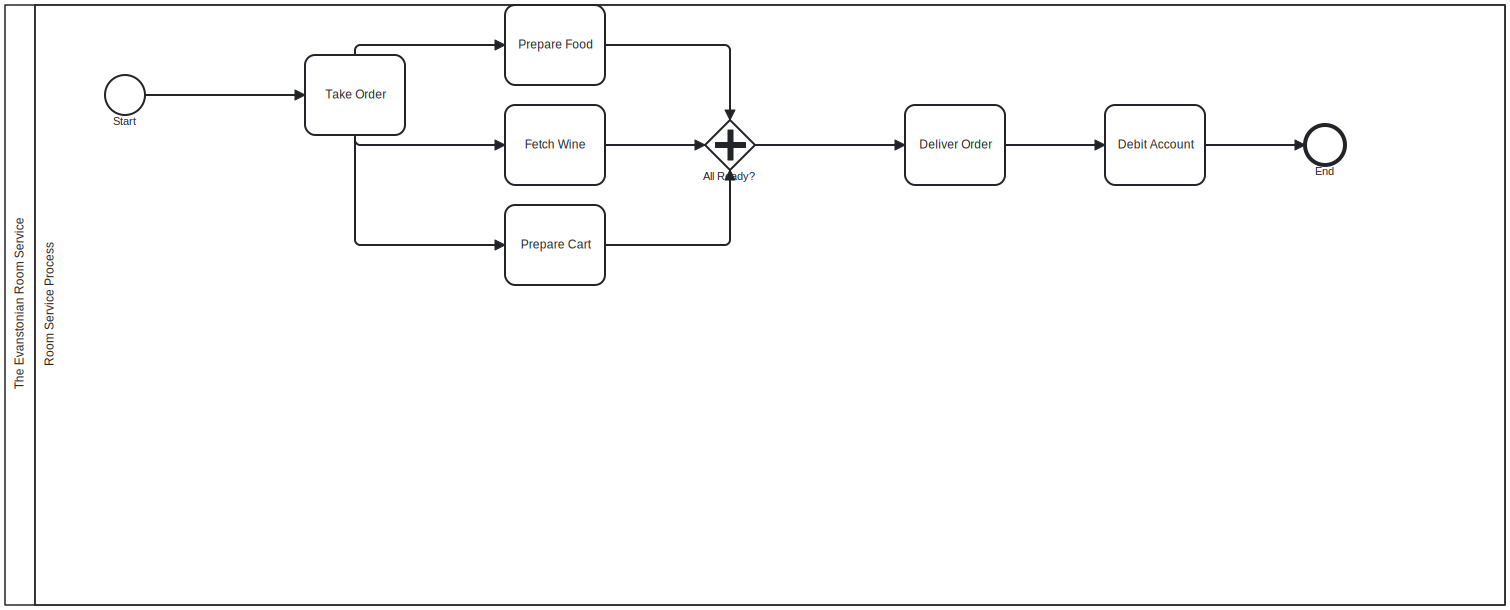
\includegraphics[width=\textwidth]{images/diagrams/1_3_assistant}
  \caption{Diagramm mit dem ChatGPT Assistant}
  \label{fig:dia-assistant}
\end{figure}

\begin{figure}[!htb]
  \centering
  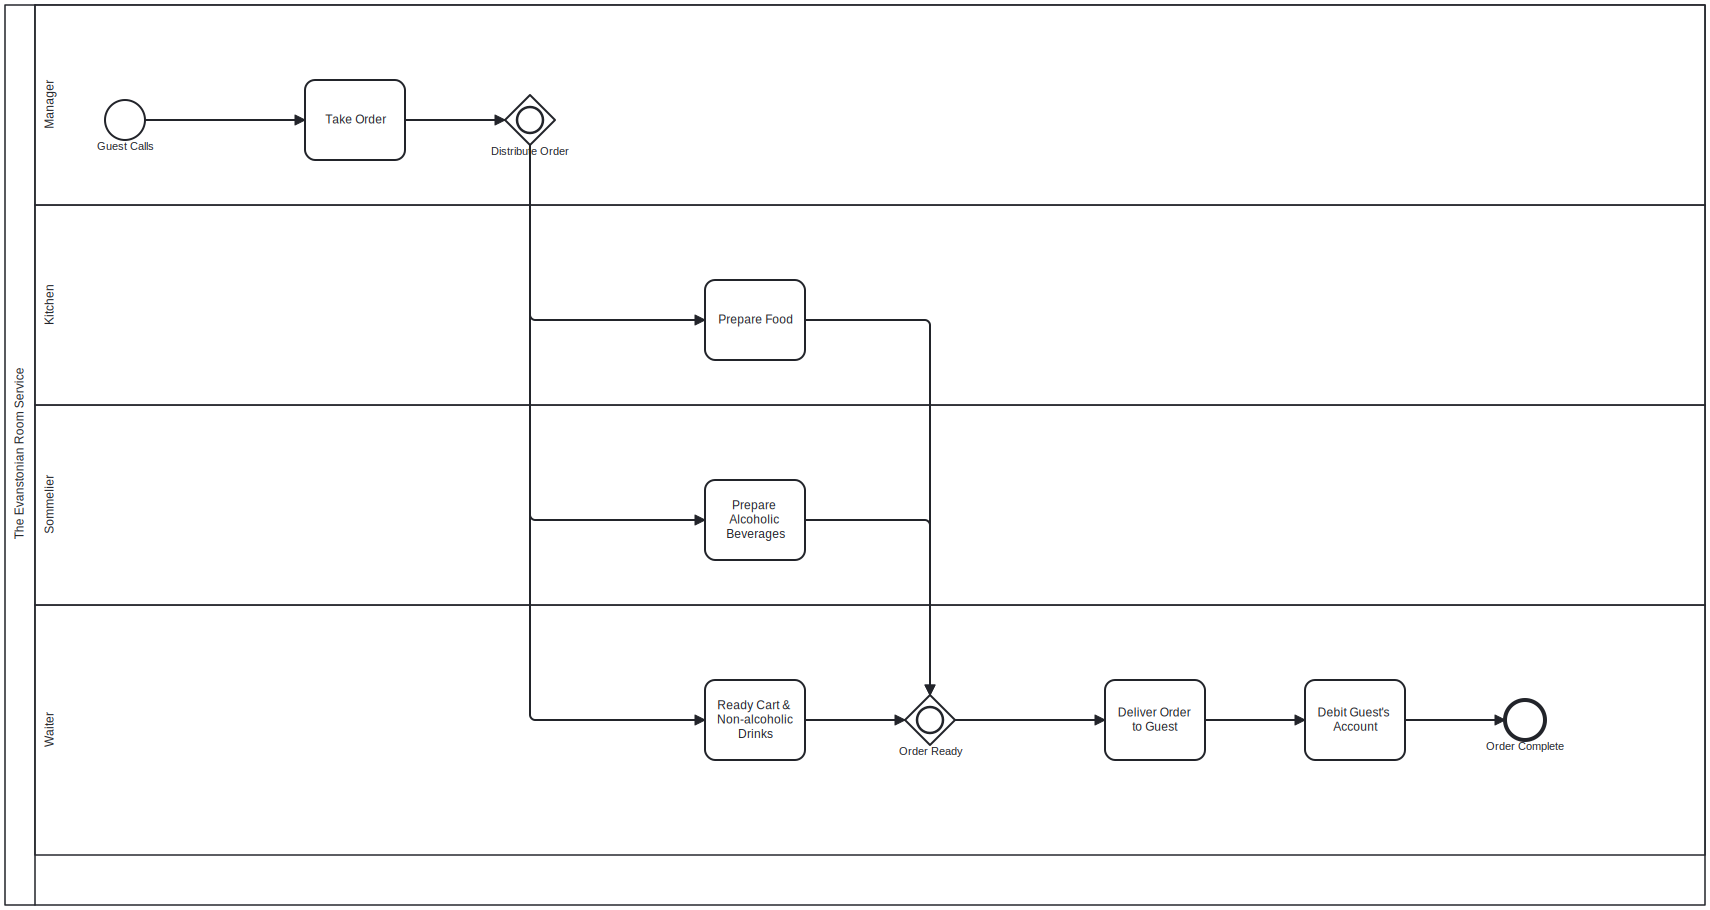
\includegraphics[width=\textwidth]{images/diagrams/1_3_json}
  \caption{Diagramm mit der Responses API und JSON Format}
  \label{fig:dia-responses-json}
\end{figure}

\begin{figure}[!htb]
  \centering
  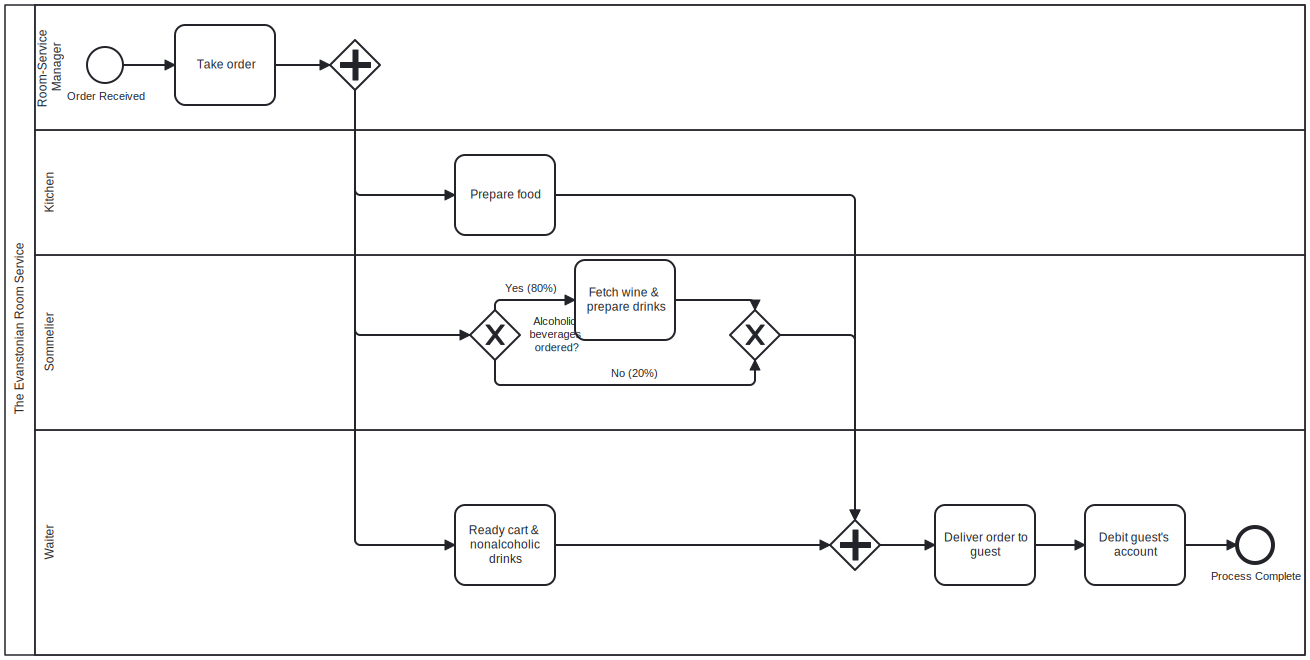
\includegraphics[width=\textwidth]{images/diagrams/1_3_xml}
  \caption{Diagramm mit der Responses API und XML Format}
  \label{fig:dia-responses-xml}
\end{figure}

\begin{figure}[!htb]
  \centering
  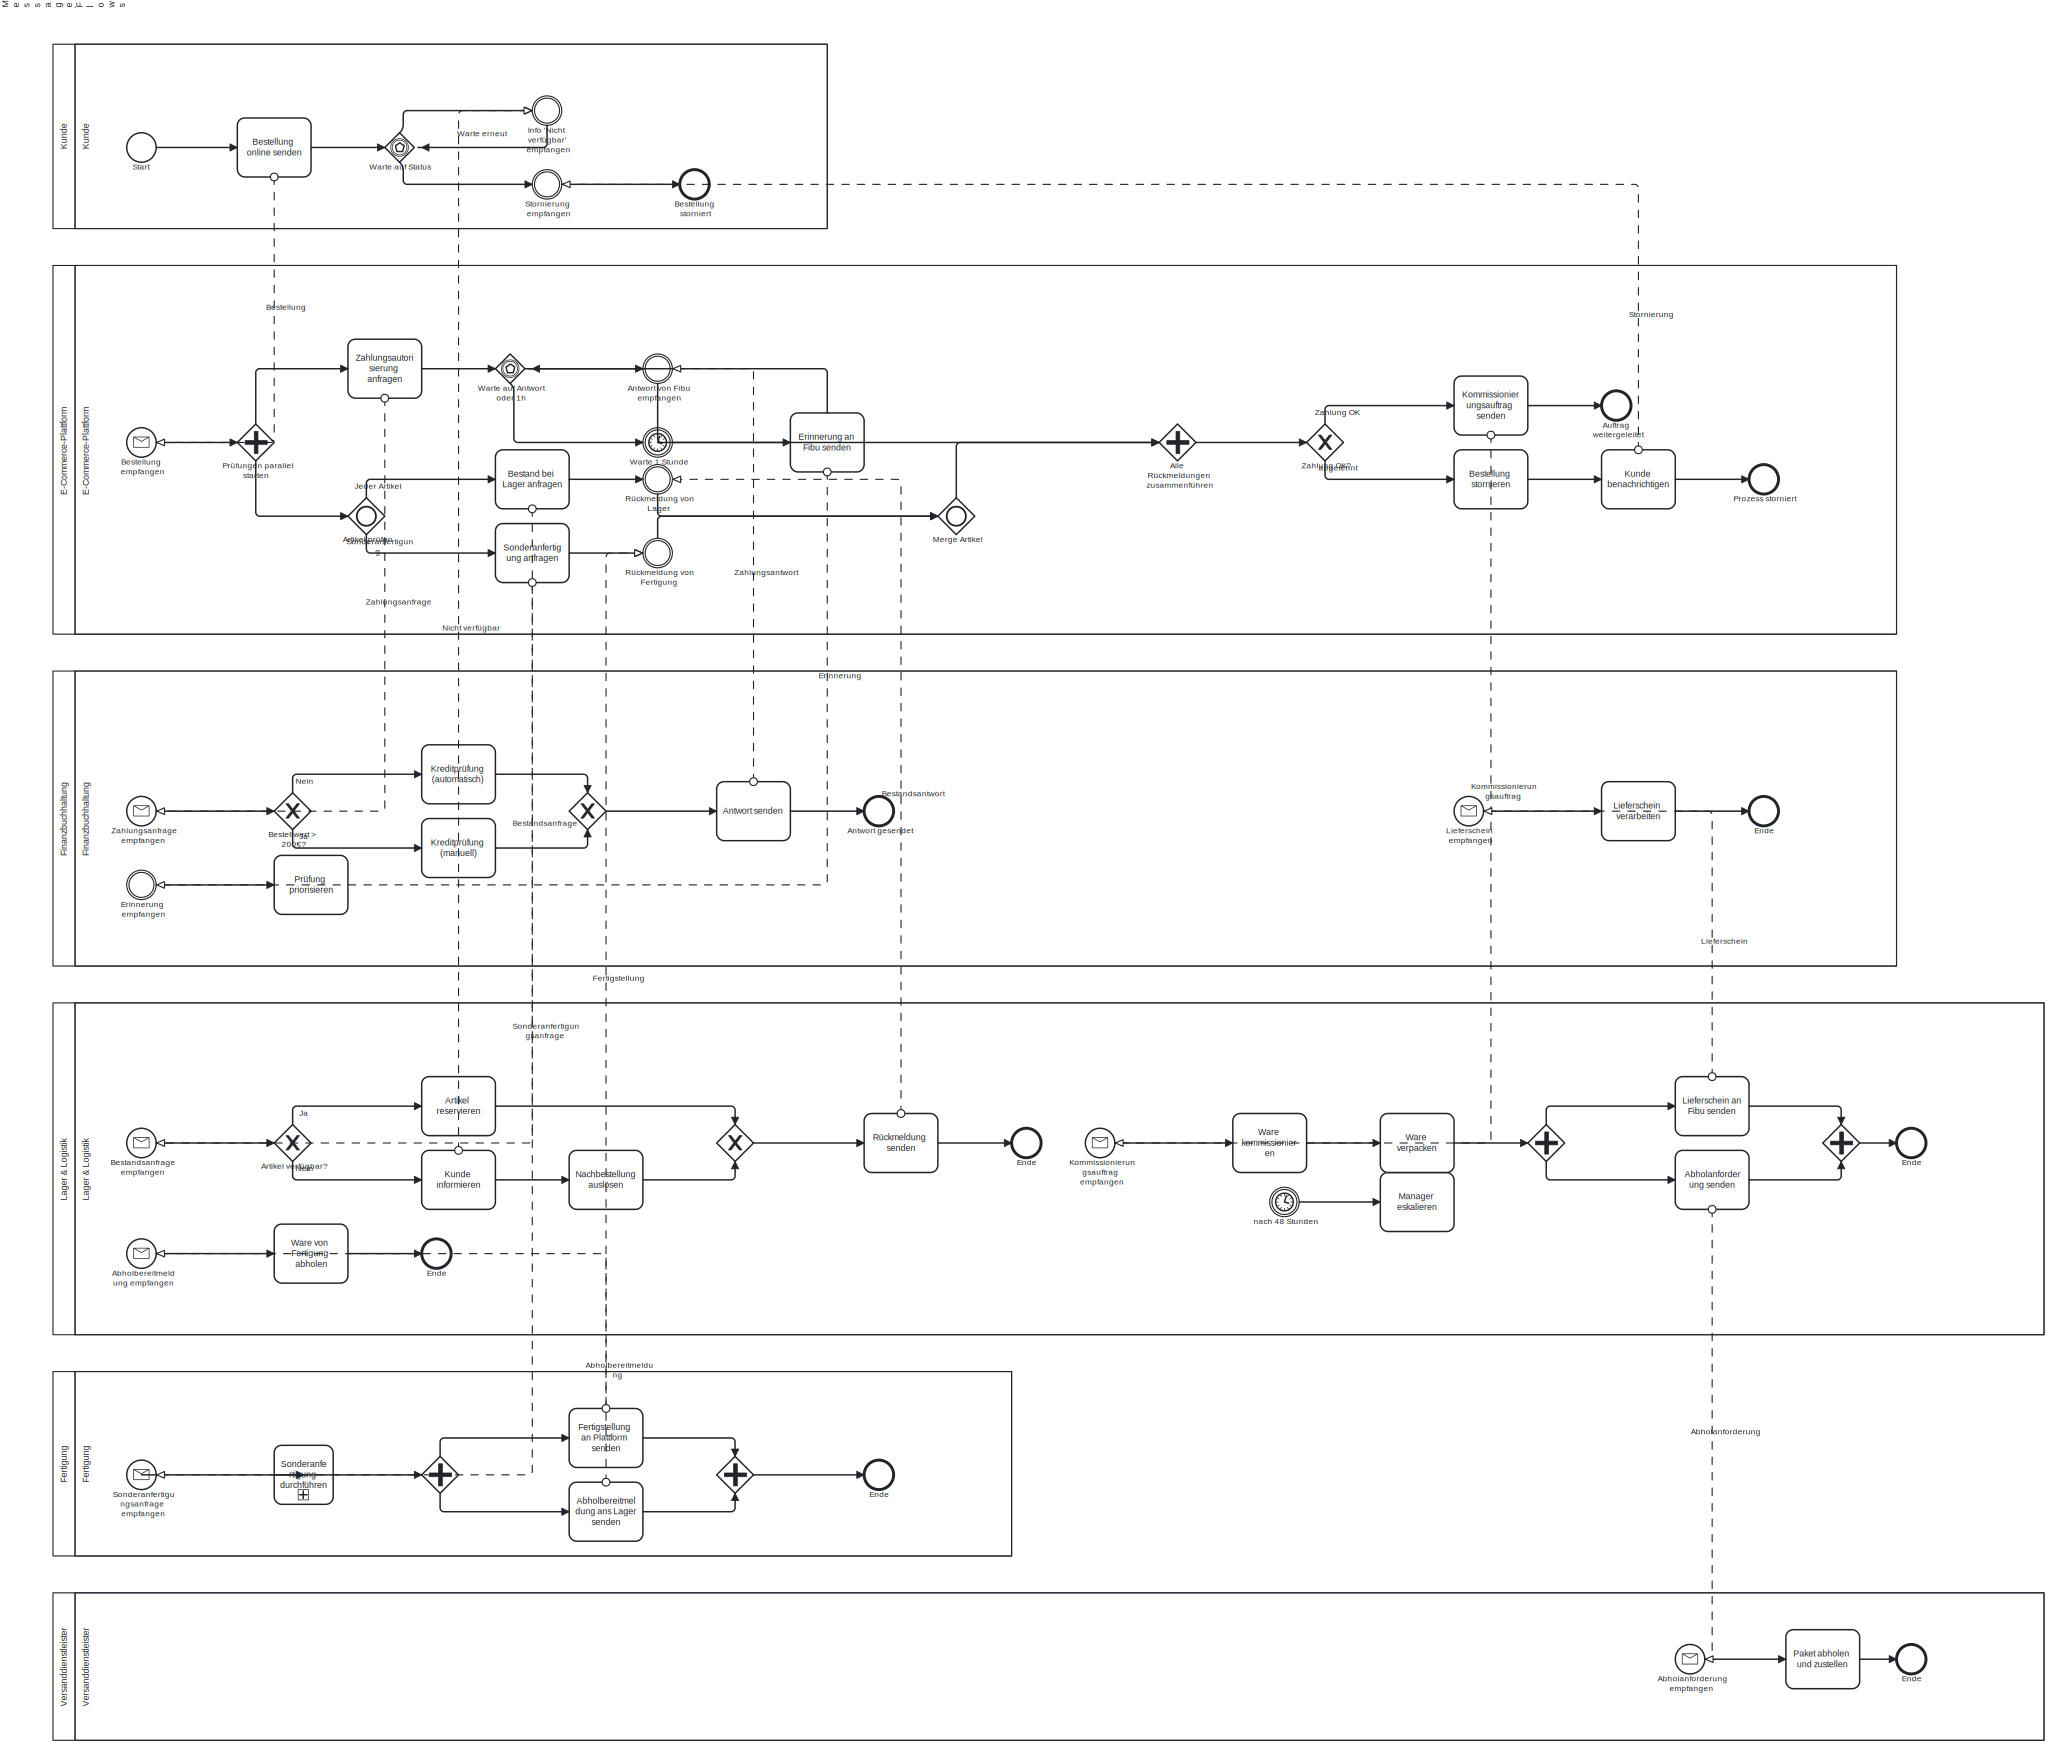
\includegraphics[width=\textwidth]{images/diagrams/gemini-2.5-pro-(json)-43sovbi9}
  \caption{Diagramm von Gemini 2.5 Pro mit JSON \\ 11904 TOKEN | 0.000 \$ | 134 s}
  \label{fig:gemini-2-5-pro-json}
\end{figure}

\begin{figure}[!htb]
  \centering
  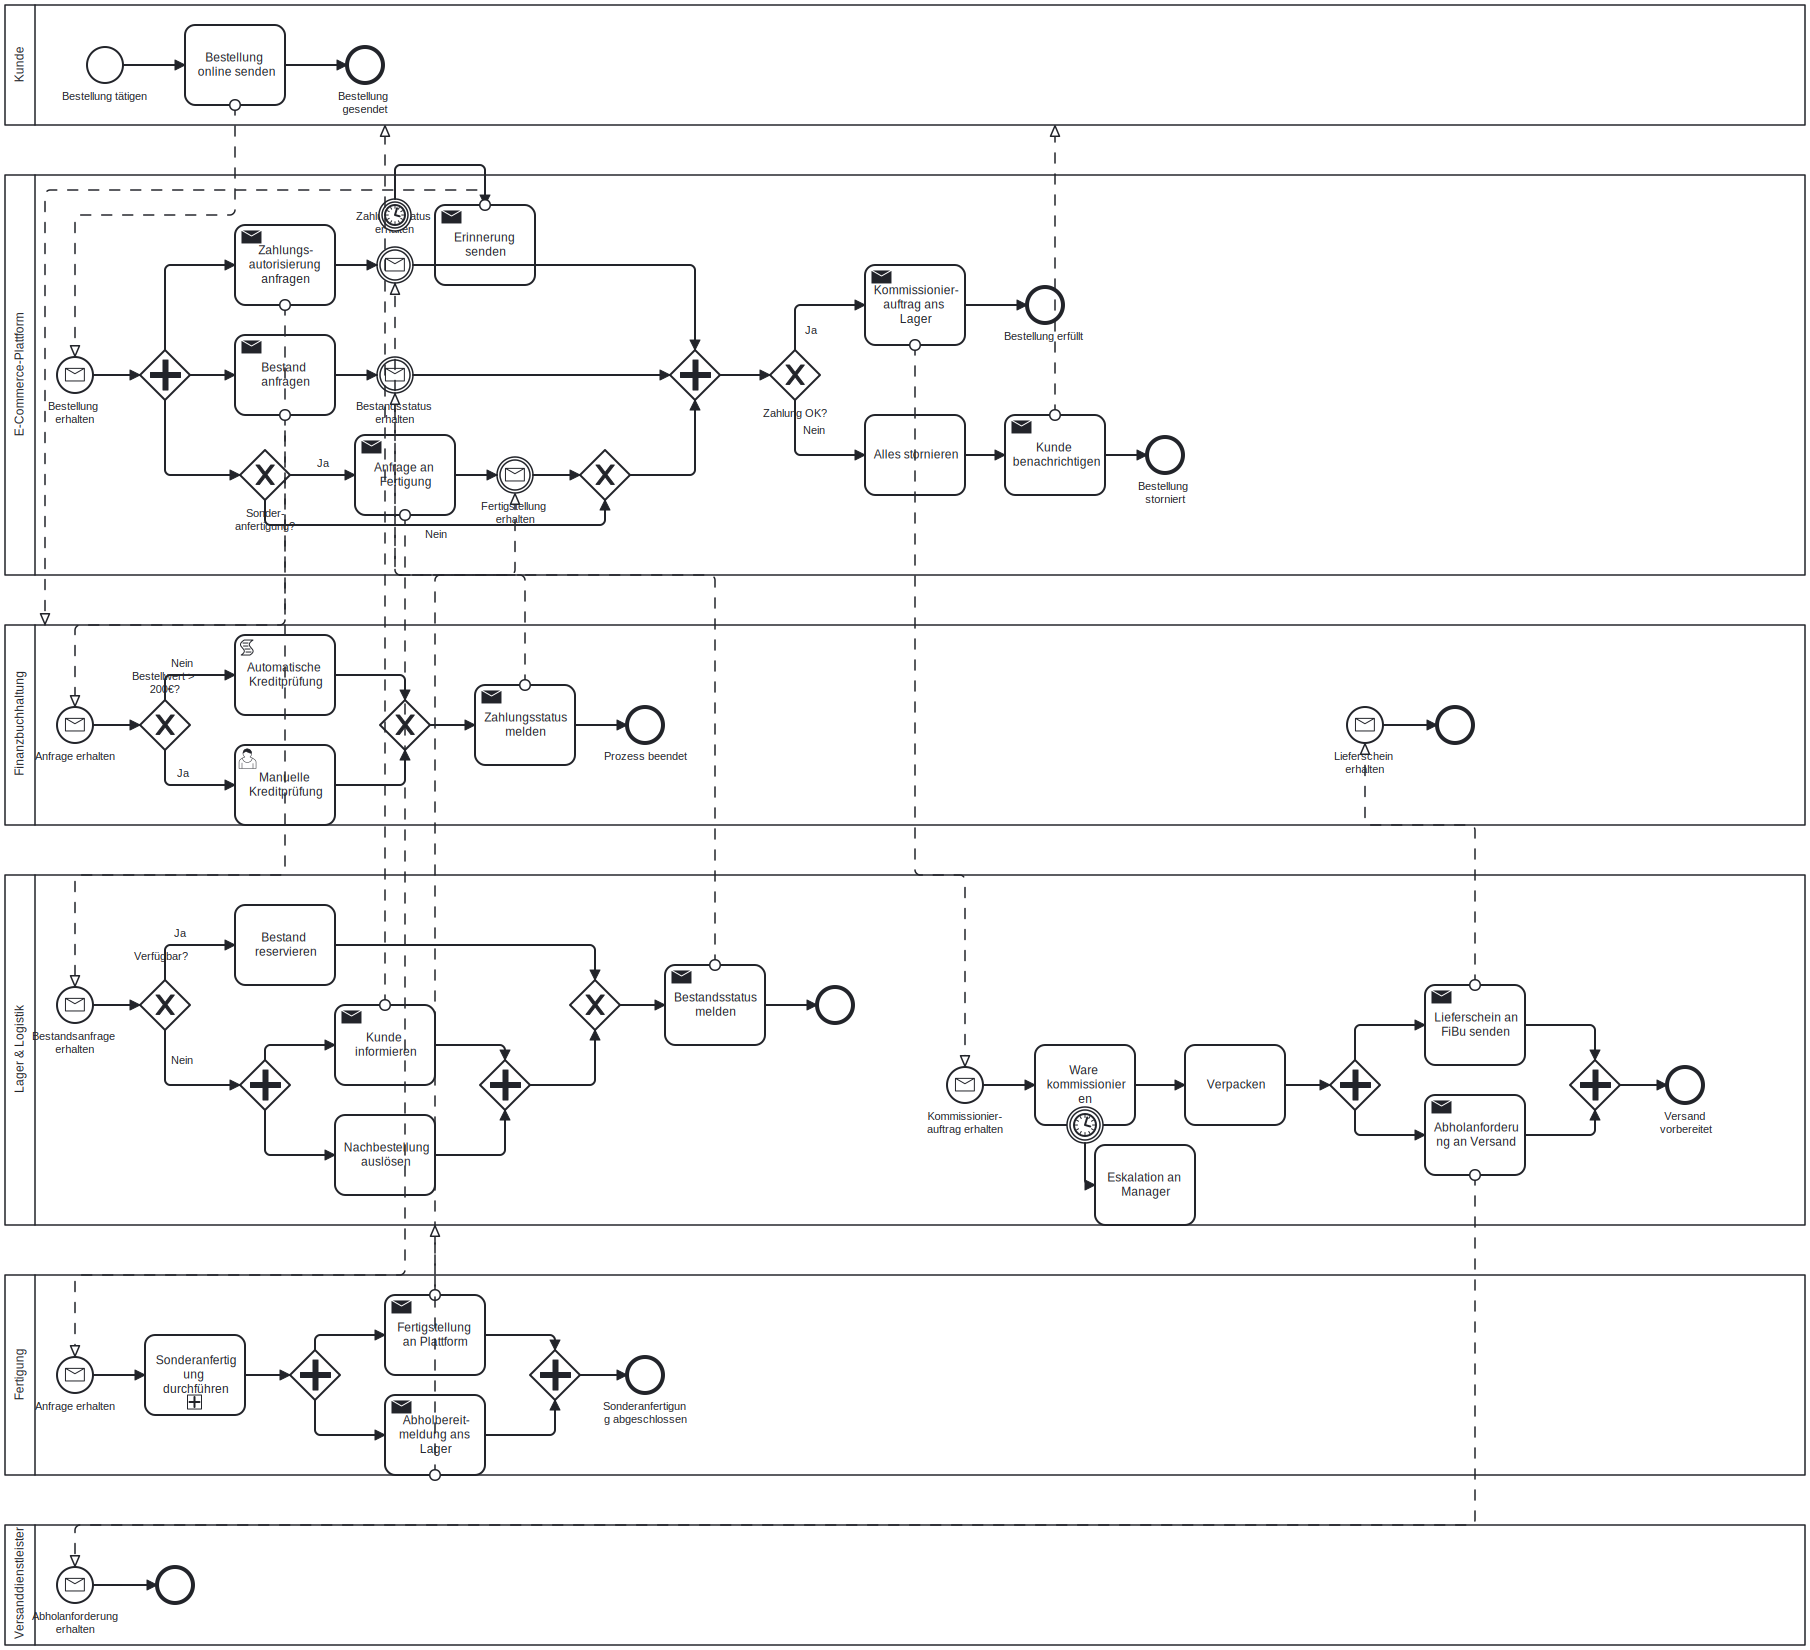
\includegraphics[width=\textwidth]{images/diagrams/gemini-2.5-pro-(xml)-m34yodi6}
  \caption{Diagramm von Gemini 2.5 Pro mit XML \\ 21183 TOKEN | 0.000 \$ | 180 s}
  \label{fig:gemini-2-5-pro-xml}
\end{figure}

\begin{figure}[!htb]
  \centering
  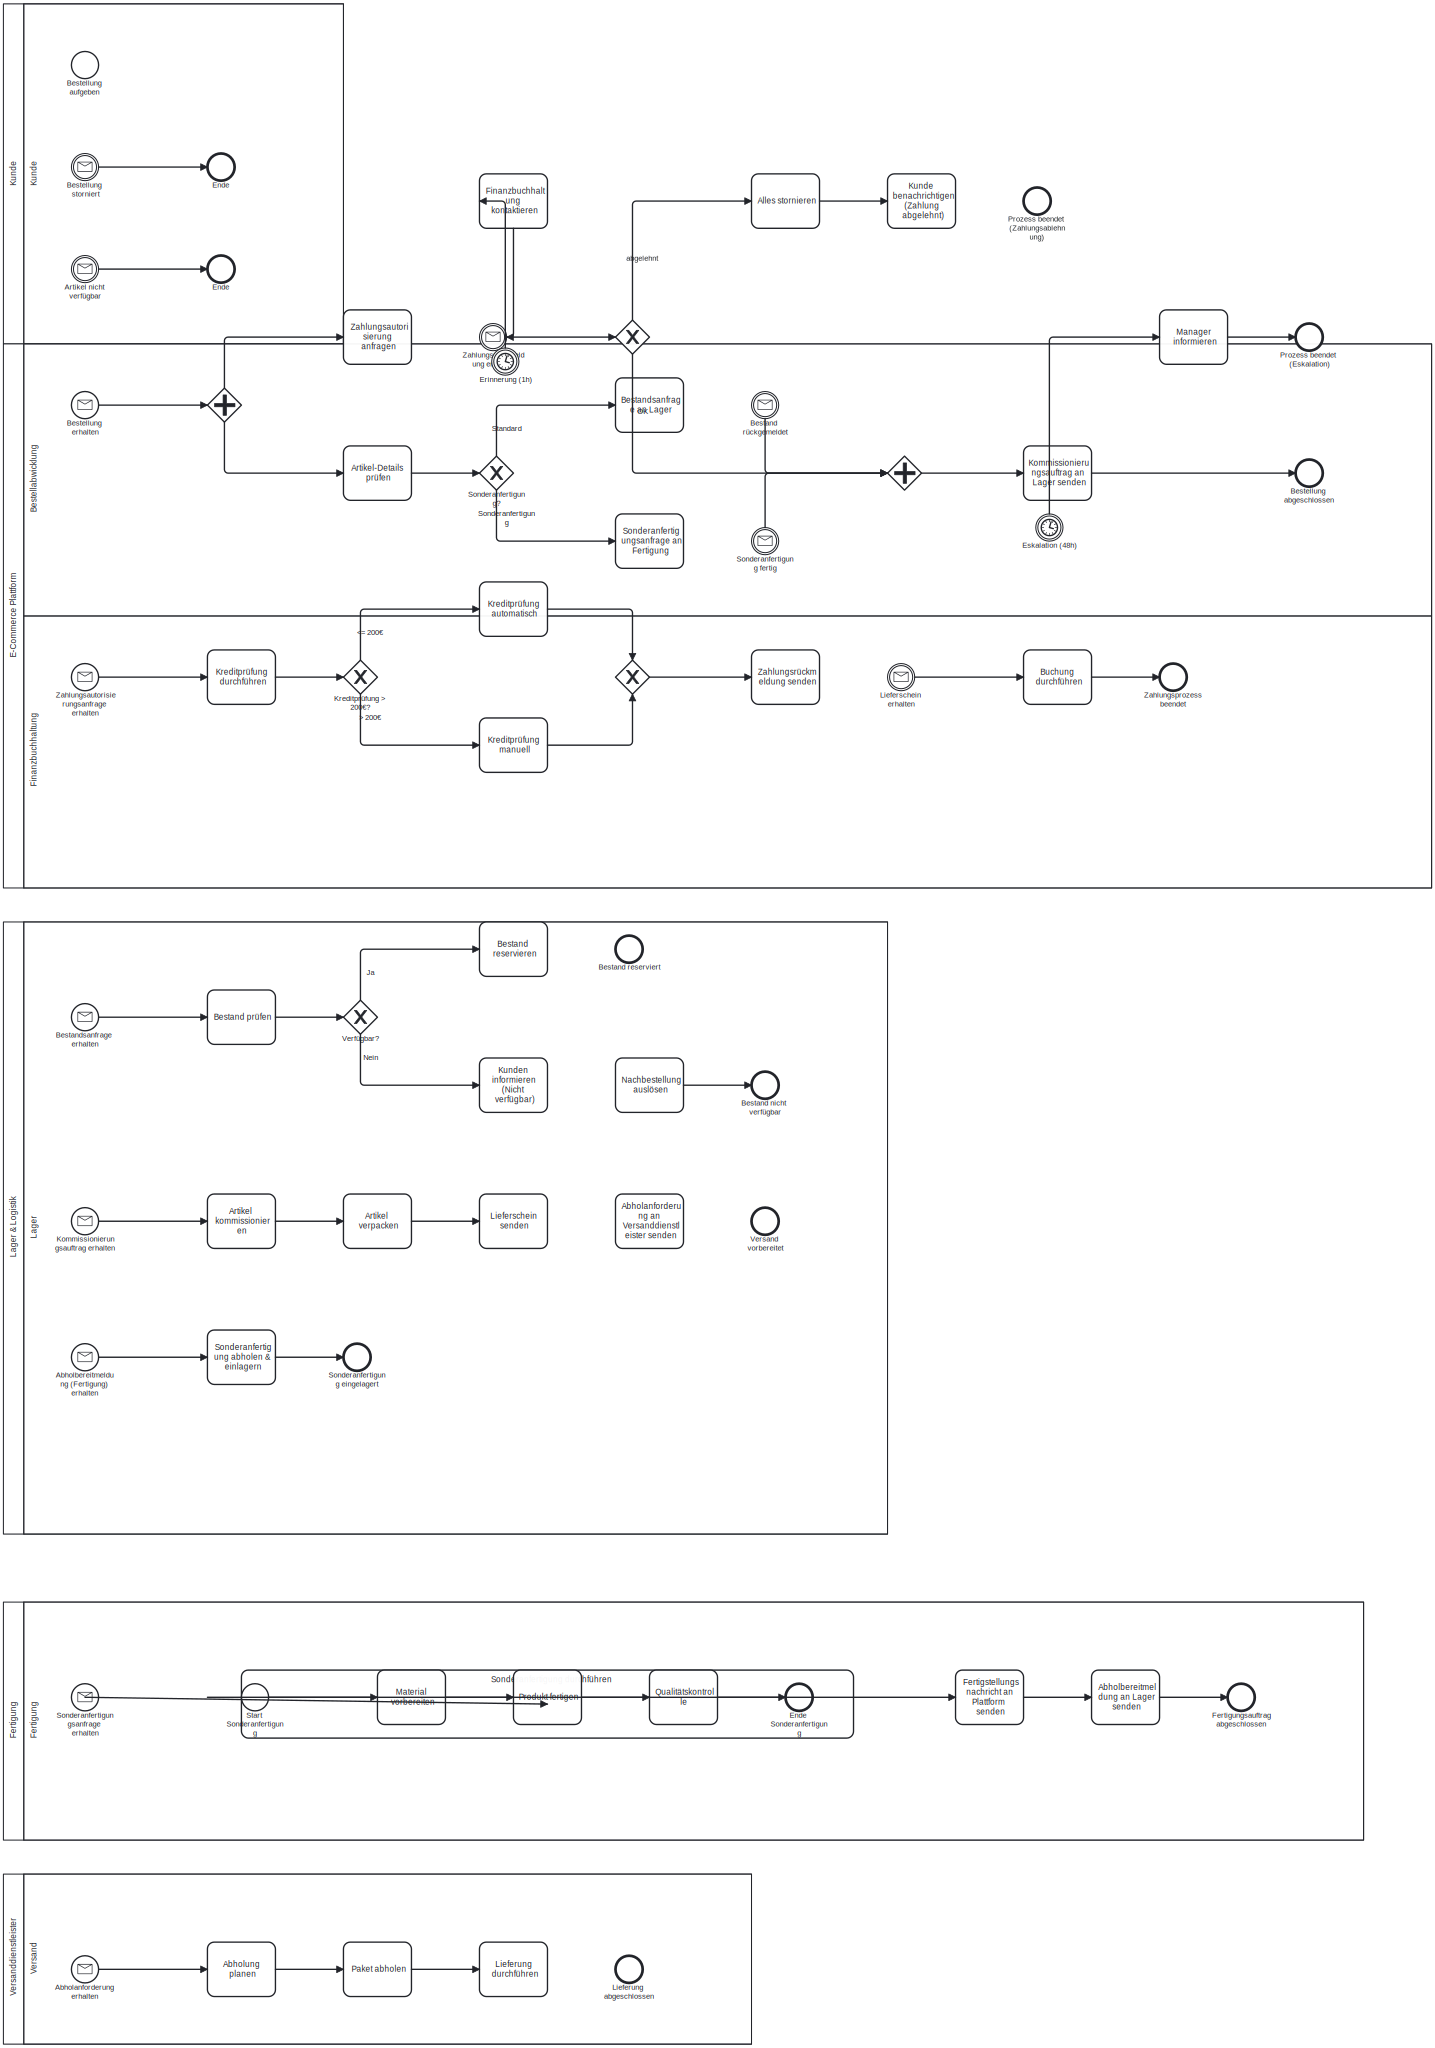
\includegraphics[height=.9\textheight]{images/diagrams/gemini-2.5-flash-(json)-vsaxxdmn}
  \caption{Diagramm von Gemini 2.5 Flash mit JSON \\ 11814 TOKEN | 0.000 \$ | 104 s}
  \label{fig:gemini-2-5-flash-json}
\end{figure}

\begin{figure}[!htb]
  \centering
  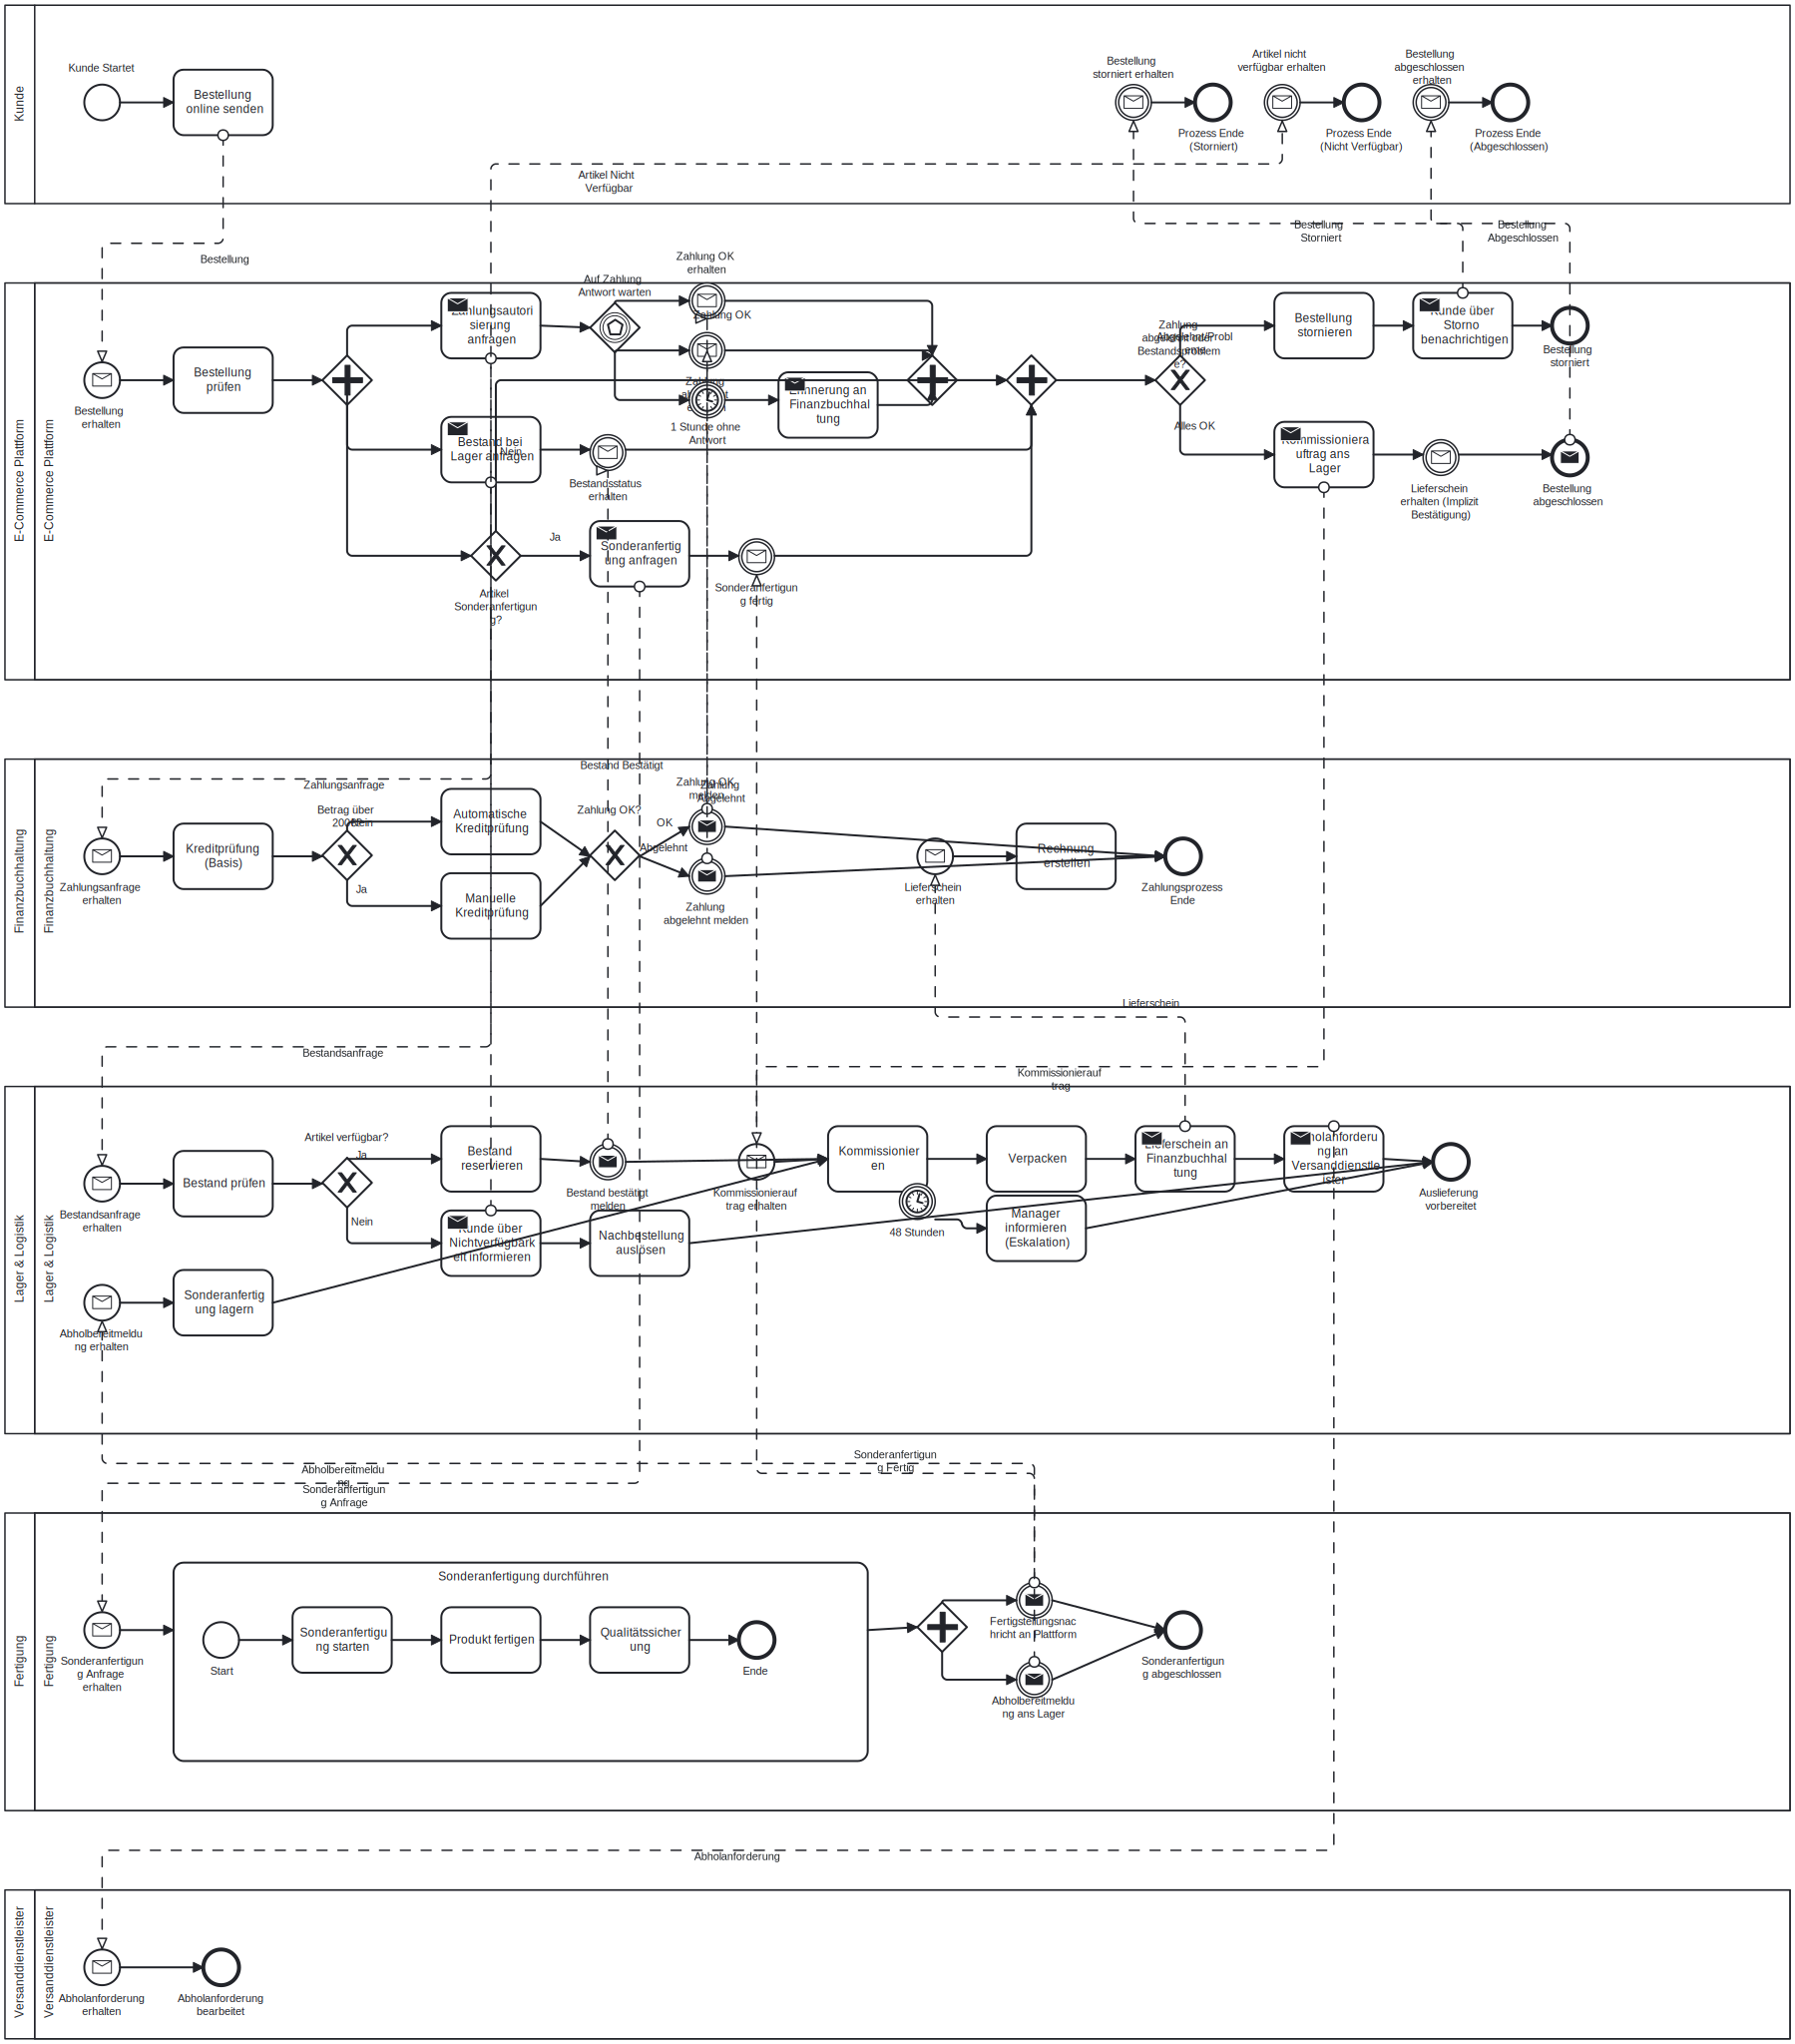
\includegraphics[width=\textwidth]{images/diagrams/gemini-2.5-flash-(xml)-epyljiqb}
  \caption{Diagramm von Gemini 2.5 Flash mit XML \\ 32371 TOKEN | 0.000 \$ | 174 s}
  \label{fig:gemini-2-5-flash-xml}
\end{figure}

\begin{figure}[!htb]
  \centering
  \includegraphics[height=.9\textheight]{images/diagrams/gpt-5.2-(json)-0kqyads7}
  \caption{Diagramm von ChatGPT 5.2 mit JSON \\ 11391 TOKEN | 0.181 \$ | 253 s}
  \label{fig:gpt-5-2-json}
\end{figure}

\begin{figure}[!htb]
  \centering
  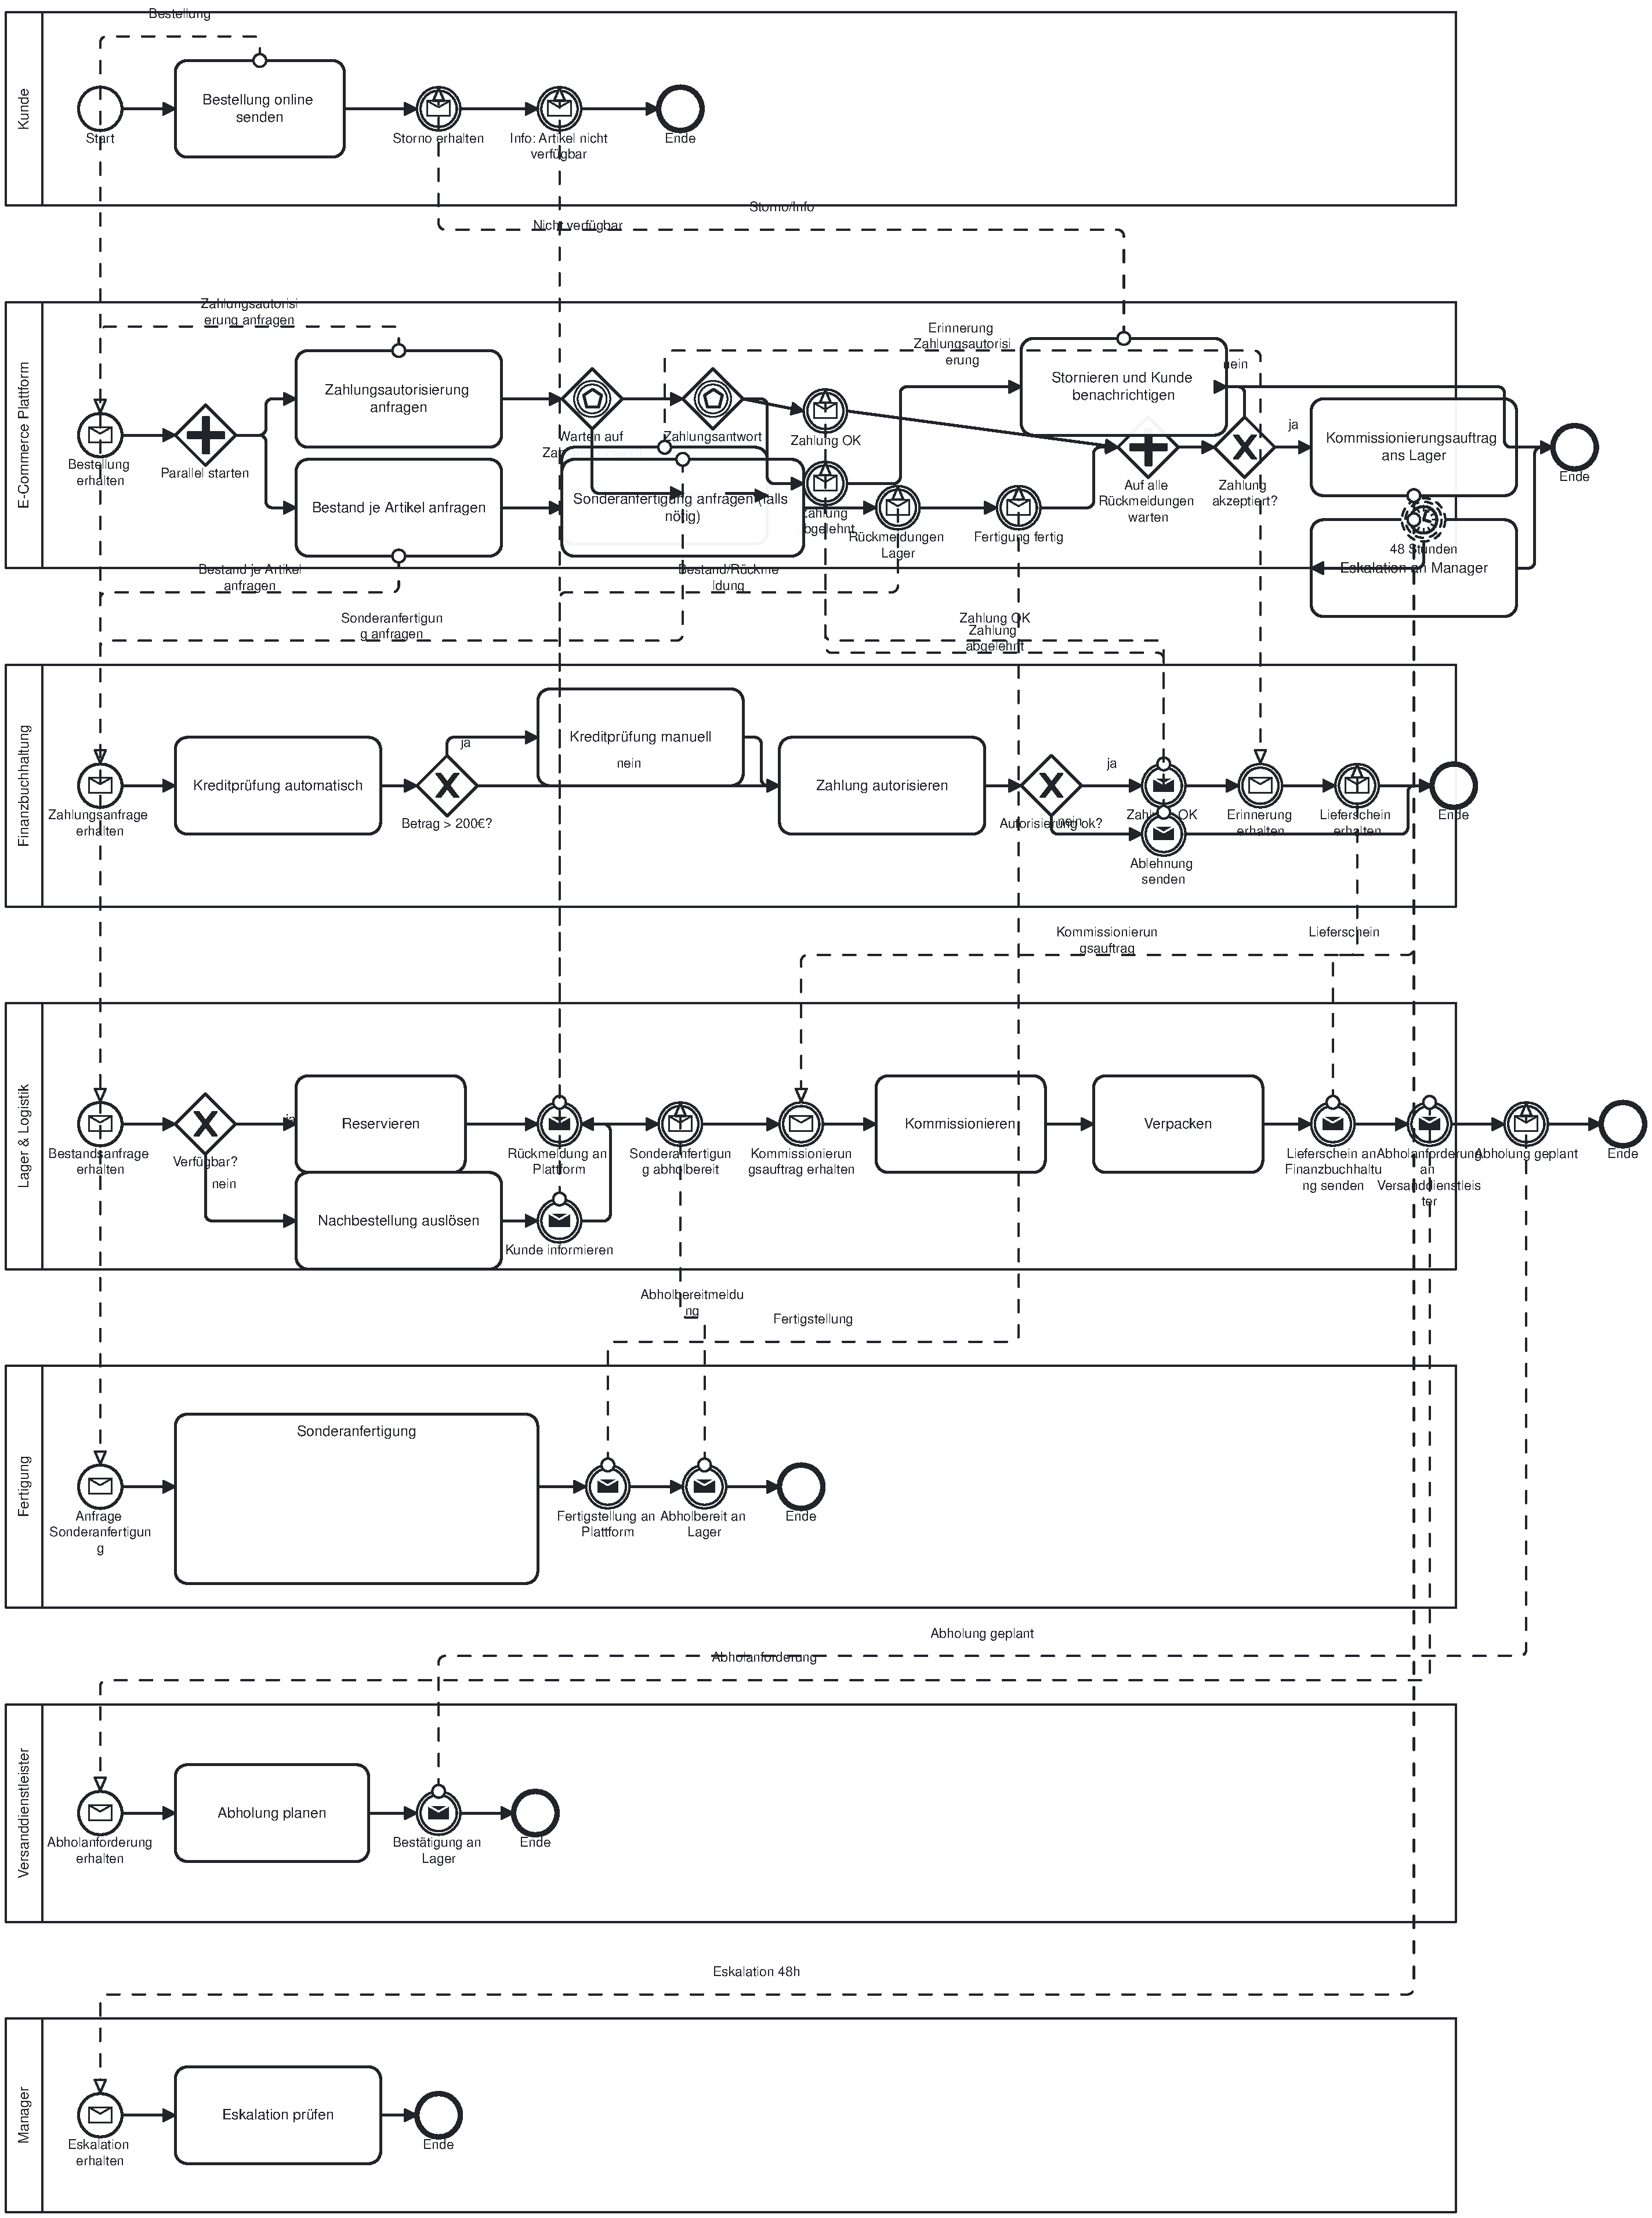
\includegraphics[width=\textwidth]{images/diagrams/gpt-5.2-(xml)-6poholbg}
  \caption{Diagramm von ChatGPT 5.2 mit XML \\ 18340 TOKEN | 0.282 \$ | 607 s}
  \label{fig:gpt-5-2-xml}
\end{figure}

\begin{figure}[!htb]
  \centering
  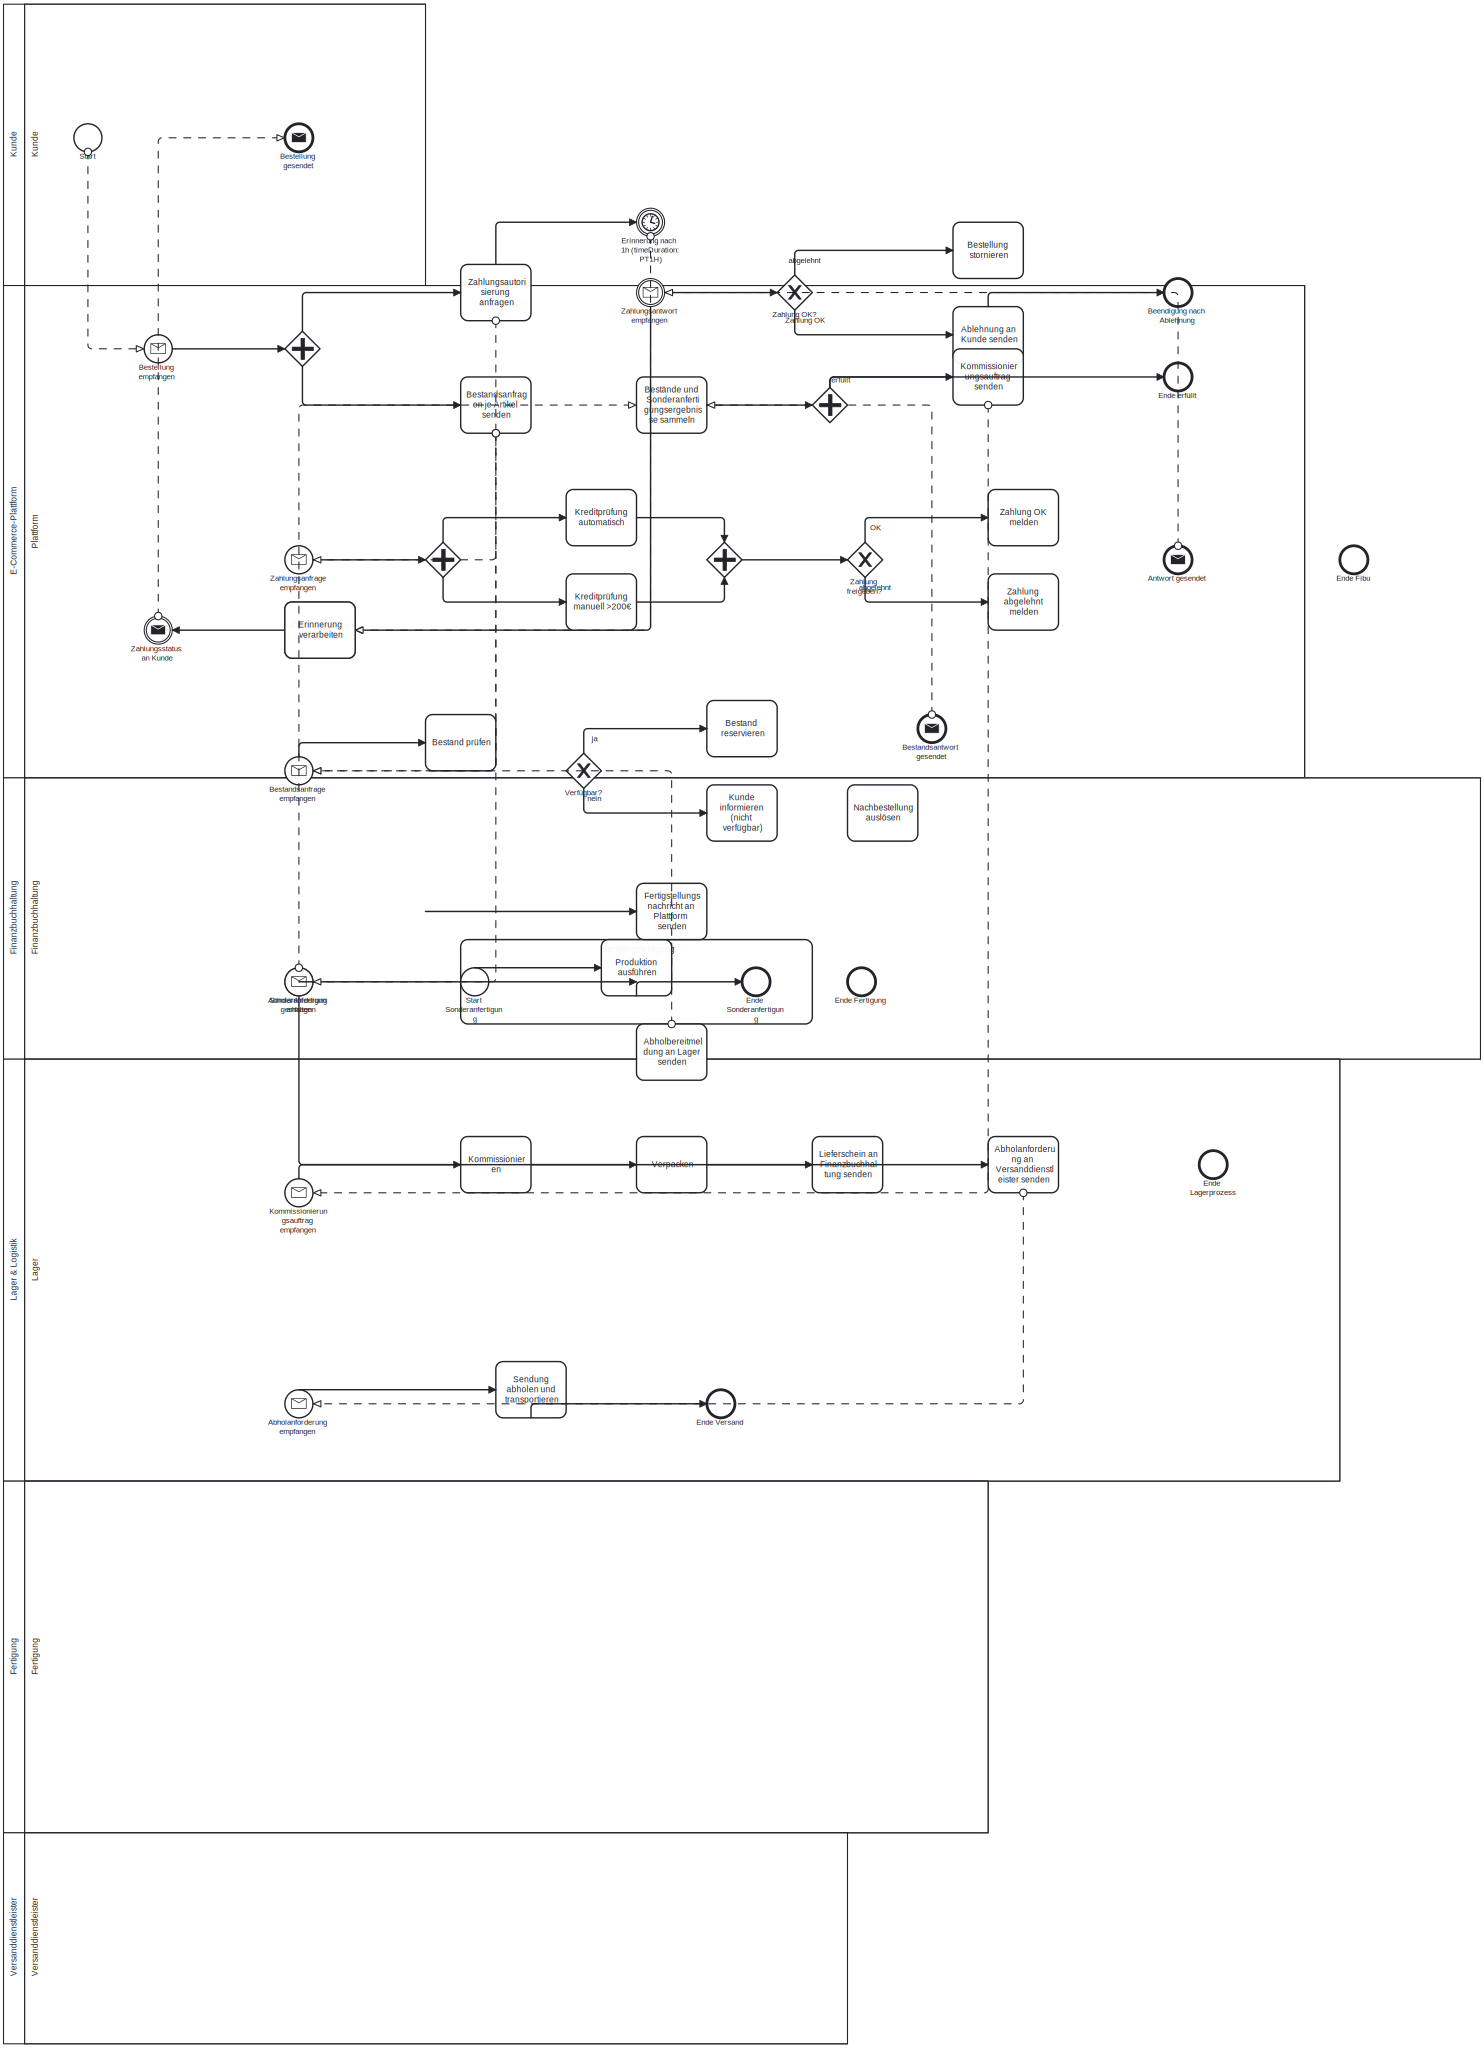
\includegraphics[height=.9\textheight]{images/diagrams/gpt-5.1-(json)-e2u2x4zb}
  \caption{Diagramm von ChatGPT 5.1 mit JSON \\ 7031 TOKEN | 0.086 \$ | 34 s}
  \label{fig:gpt-5-1-json}
\end{figure}

\begin{figure}[!htb]
  \centering
  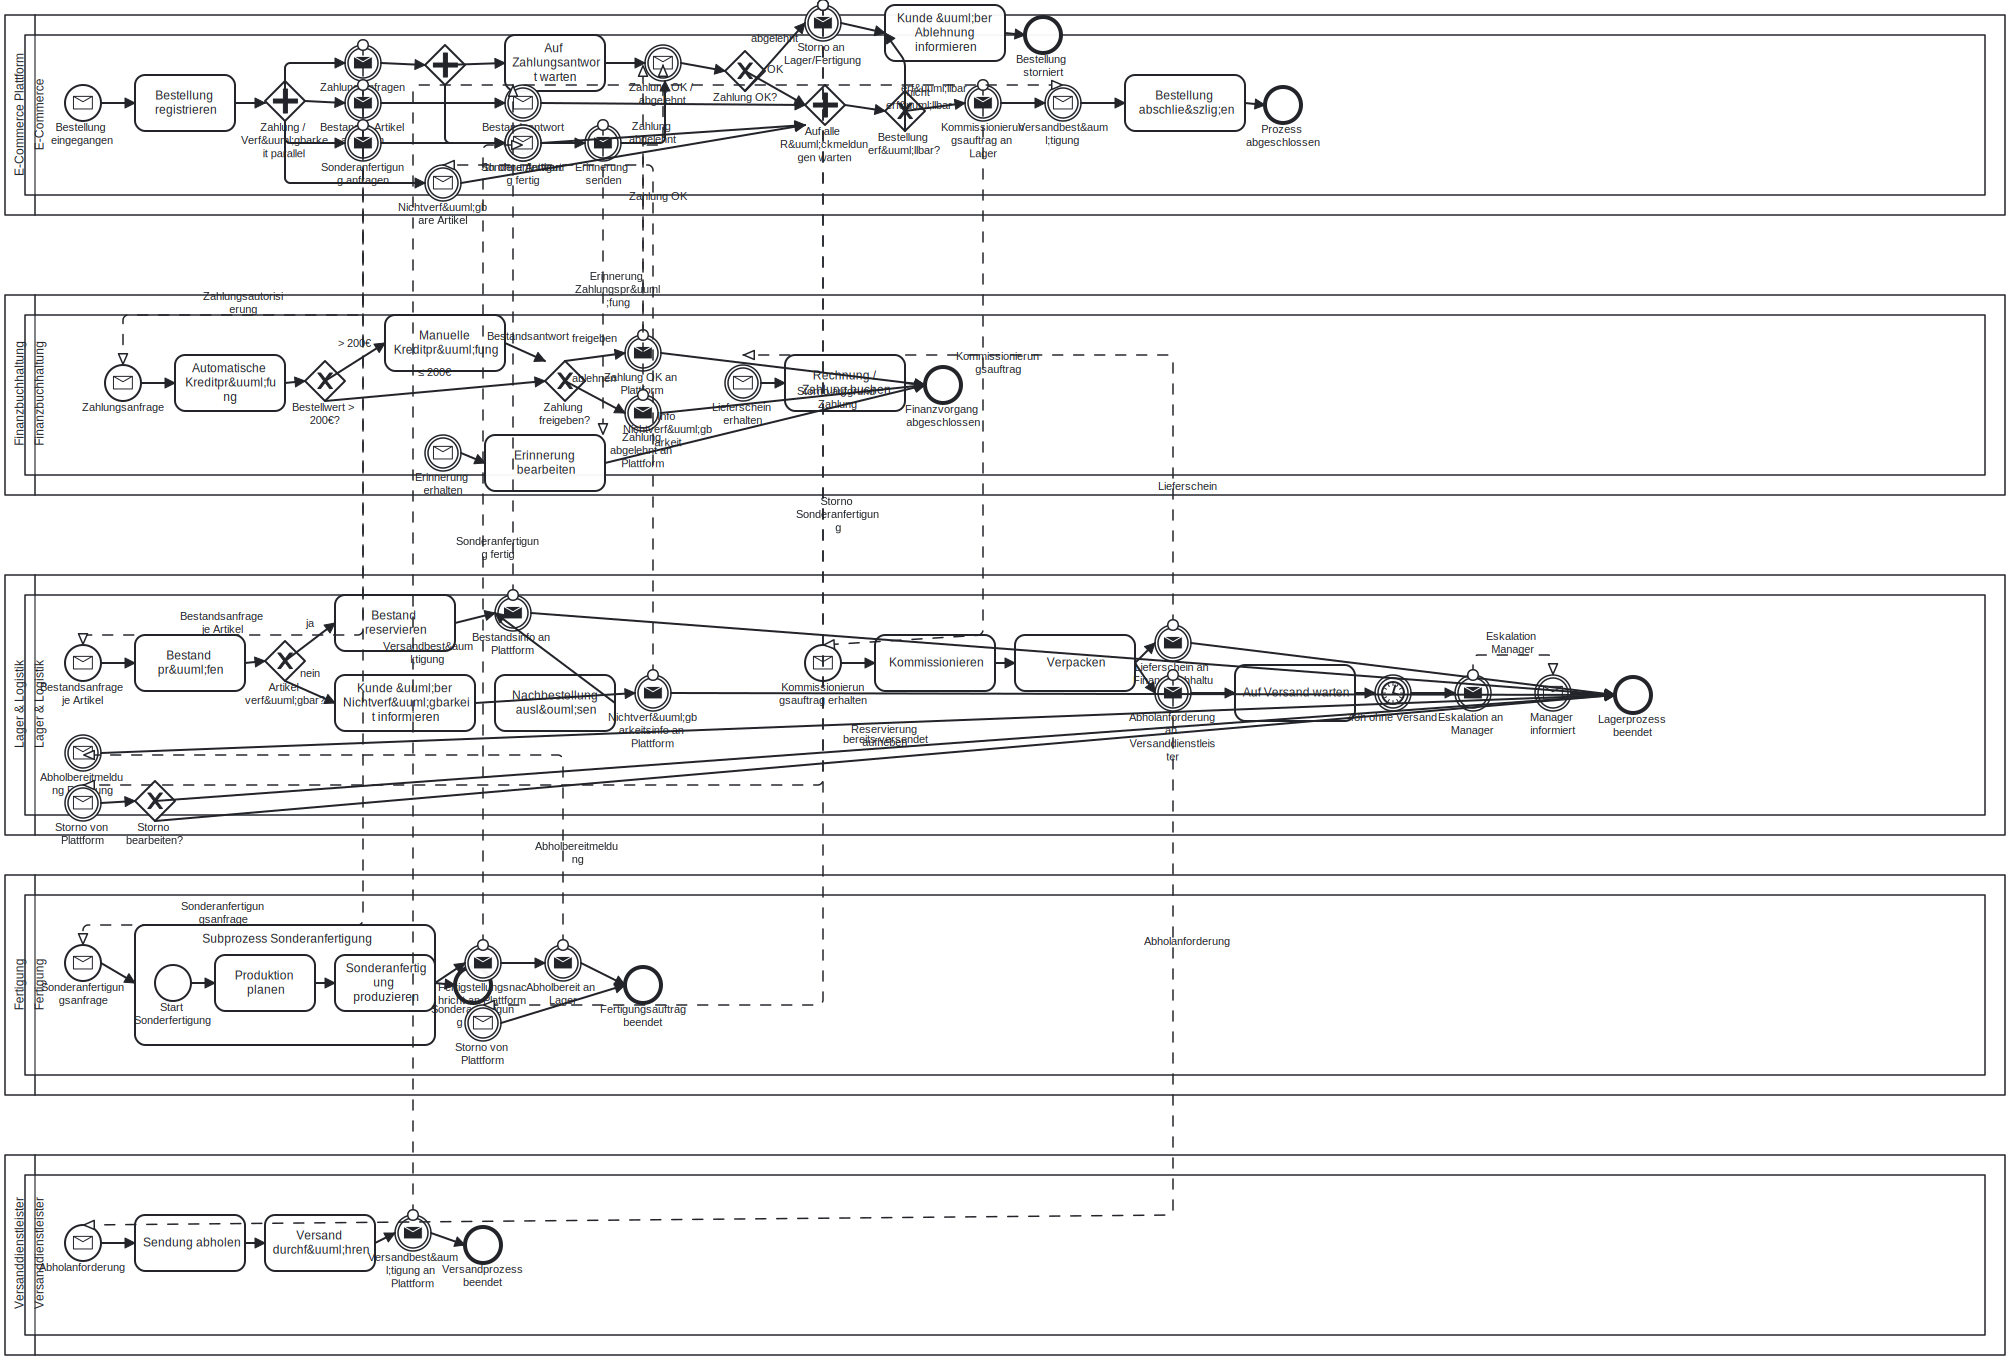
\includegraphics[width=\textwidth]{images/diagrams/gpt-5.1-(xml)-47085wam}
  \caption{Diagramm von ChatGPT 5.1 mit XML \\ 21697 TOKEN | 0.234 \$ | 105 s}
  \label{fig:gpt-5-1-xml}
\end{figure}

\begin{figure}[!htb]
  \centering
  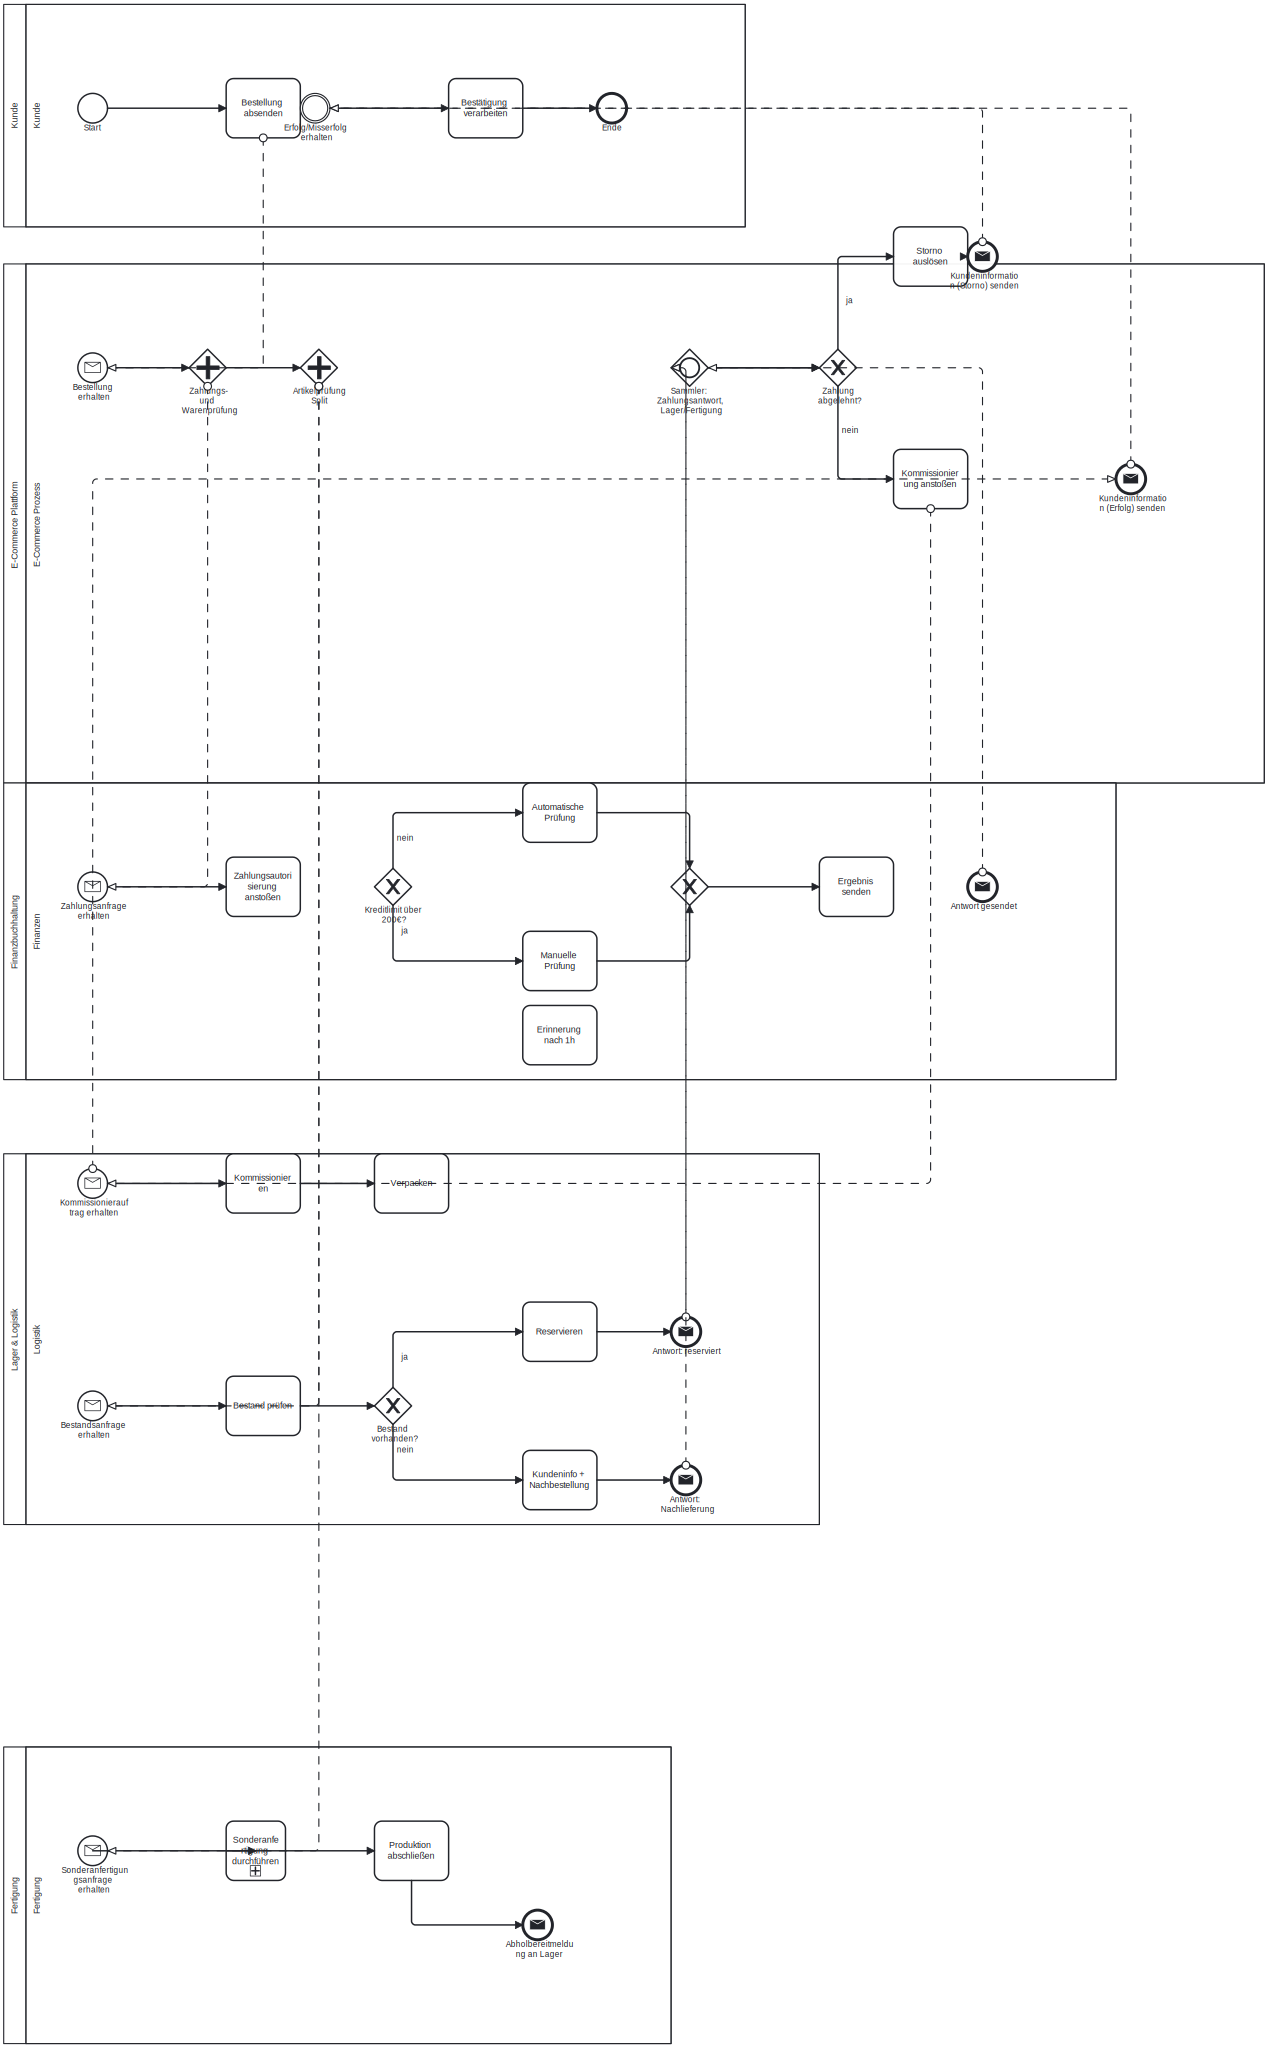
\includegraphics[height=.9\textheight]{images/diagrams/gpt-4.1-(json)-6xk6wtee}
  \caption{Diagramm von ChatGPT 4.1 mit JSON \\ 5793 TOKEN | 0.077 \$ | 69 s}
  \label{fig:gpt-4-1-json}
\end{figure}

\begin{figure}[!htb]
  \centering
  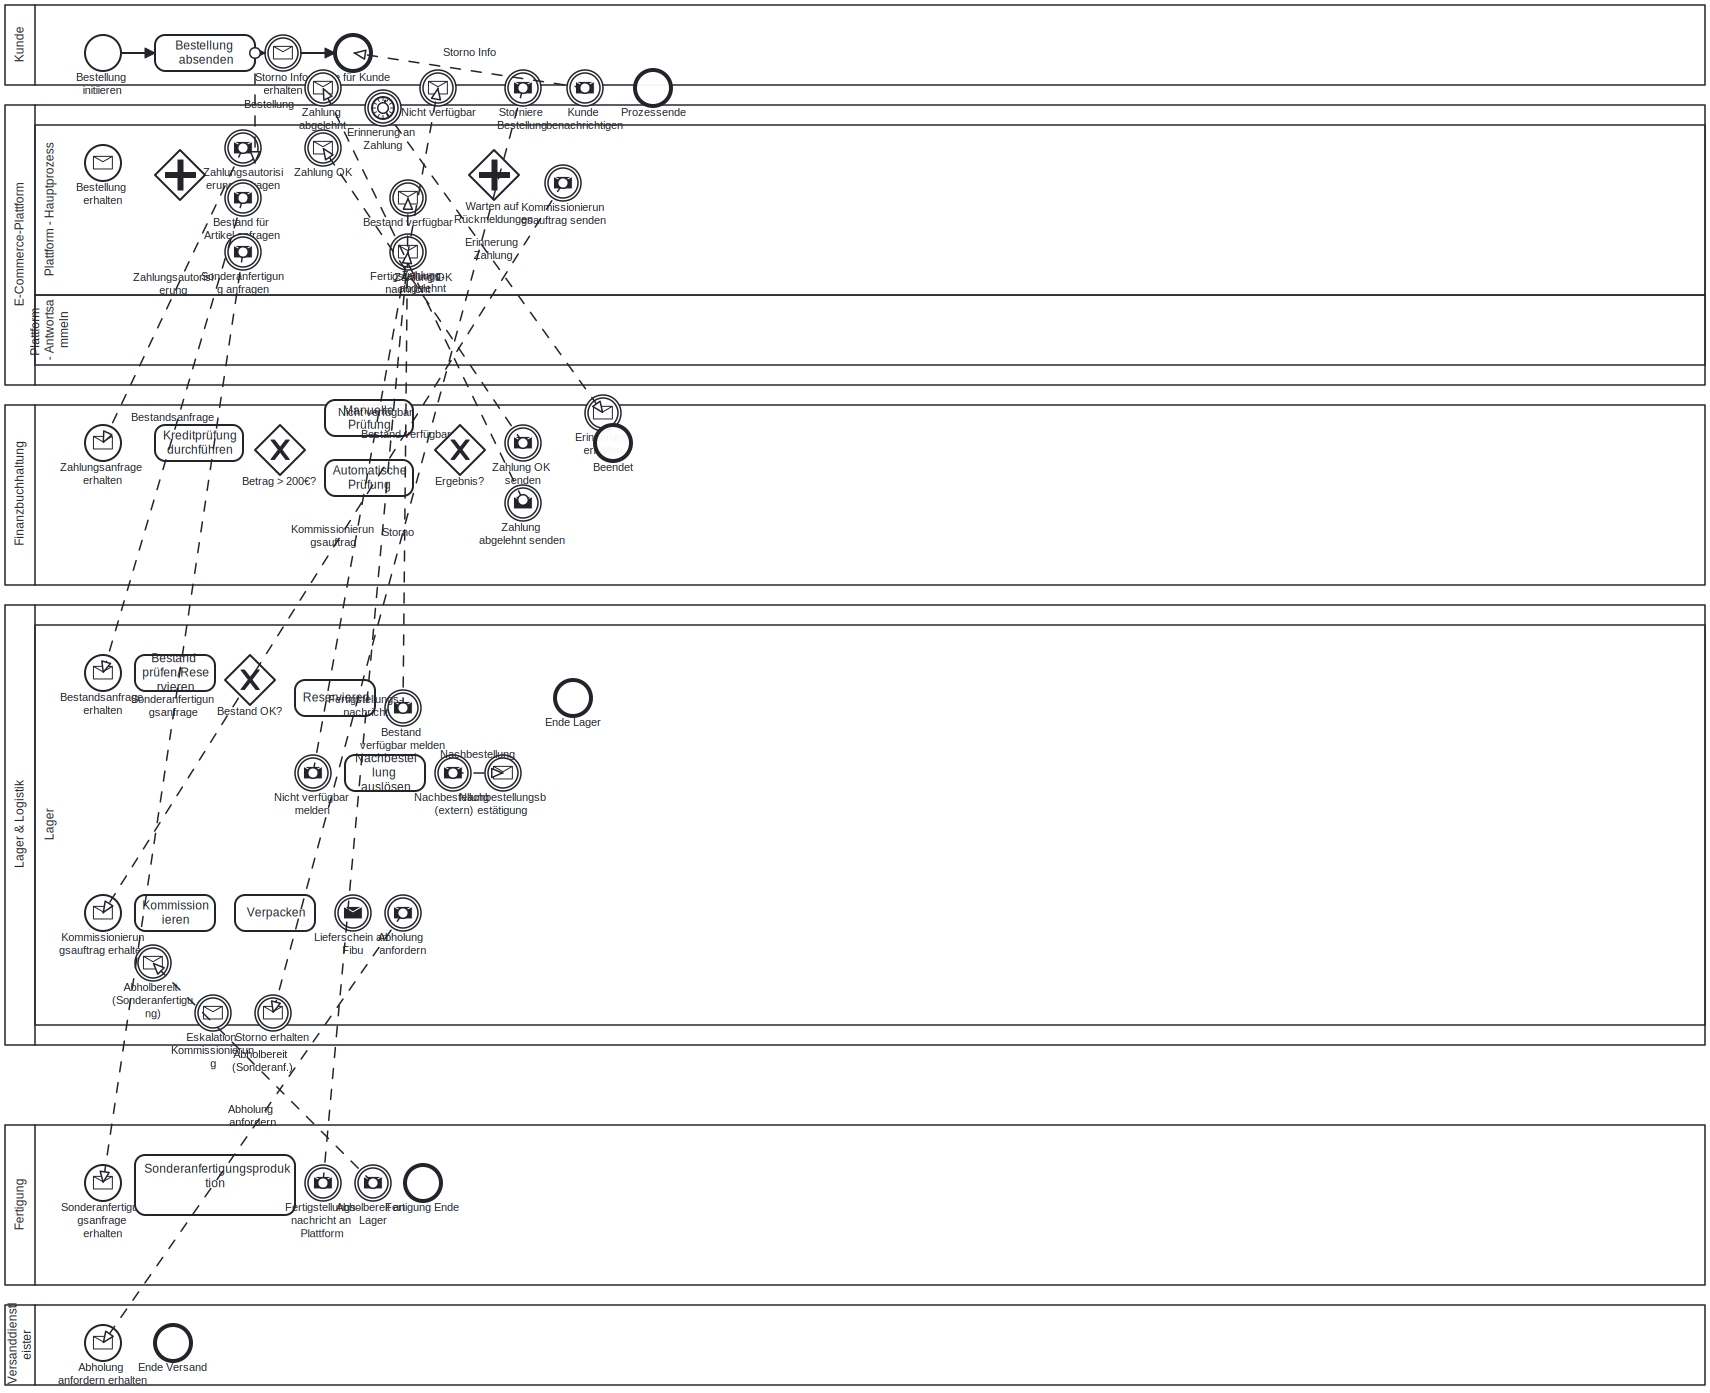
\includegraphics[width=\textwidth]{images/diagrams/gpt-4.1-(xml)-esv47un0}
  \caption{Diagramm von ChatGPT 4.1 mit XML \\ 12944 TOKEN | 0.130 \$ | 168 s}
  \label{fig:gpt-4-1-xml}
\end{figure}

\begin{figure}[!htb]
  \centering
  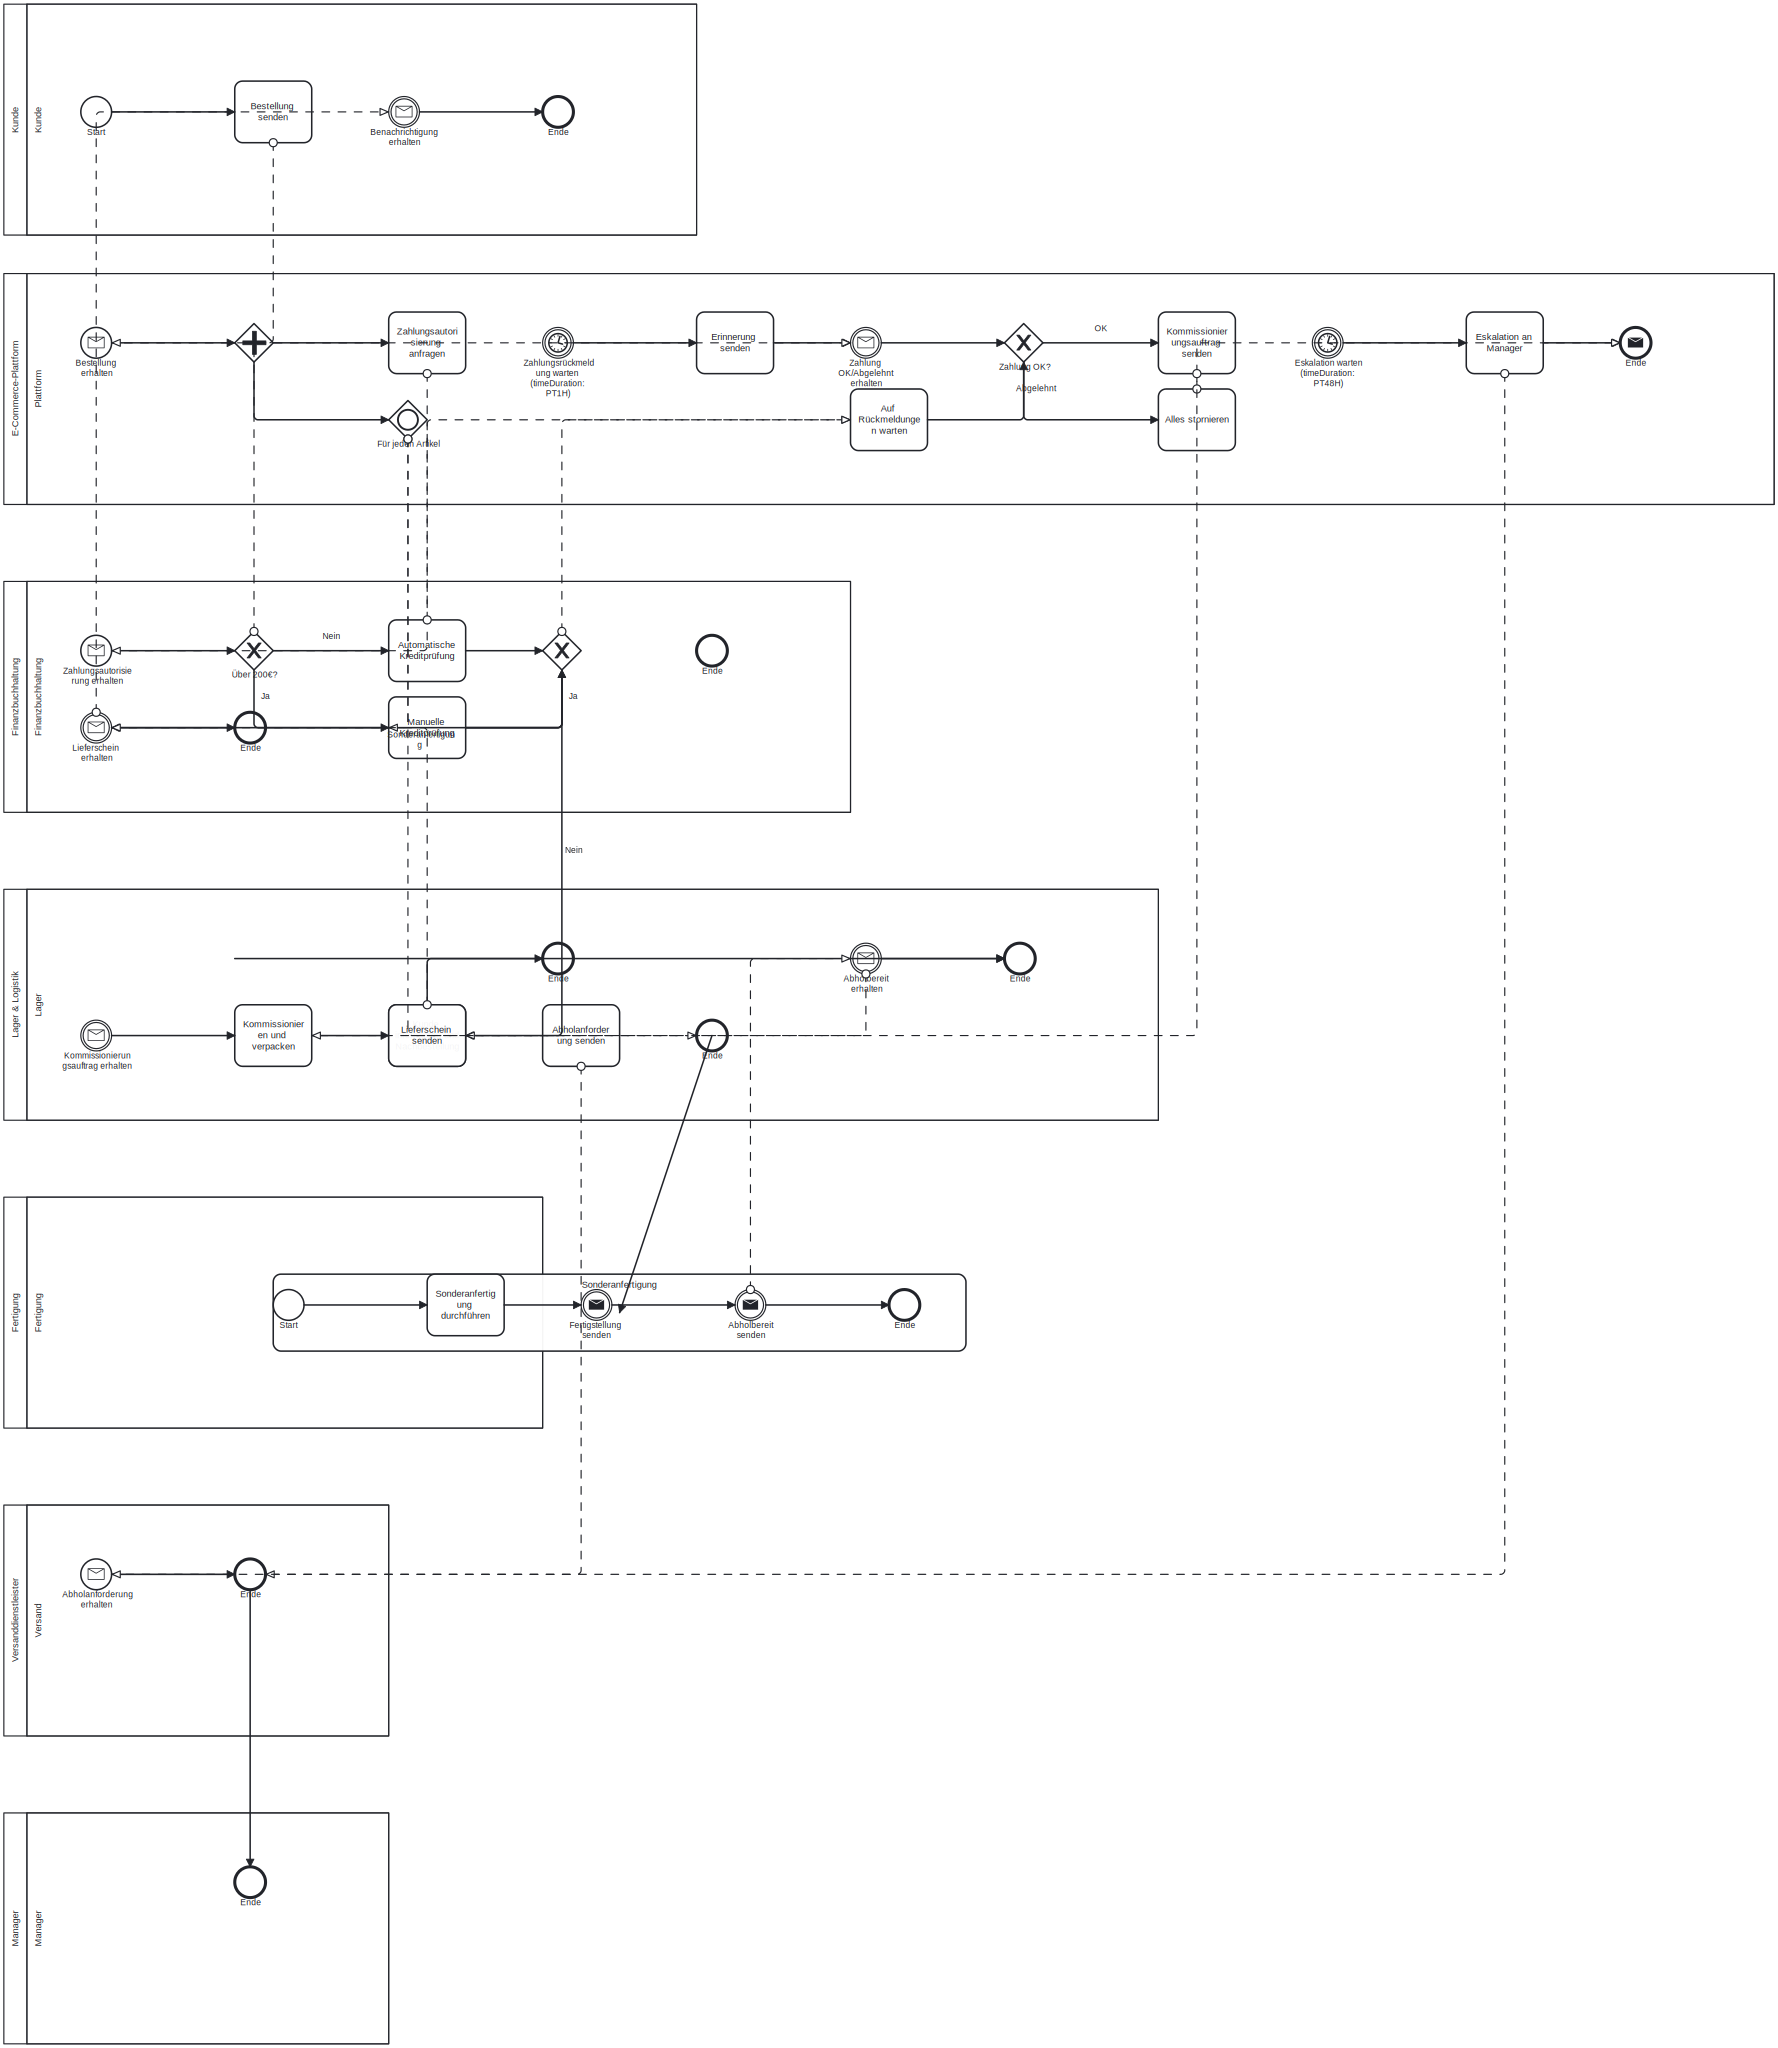
\includegraphics[width=\textwidth]{images/diagrams/grok-4-(json)-esye6wjy}
  \caption{Diagramm von Grok 4 mit JSON \\ 7263 TOKEN | 0.161 \$ | 248 s}
  \label{fig:grok-4-json}
\end{figure}

\begin{figure}[!htb]
  \centering
  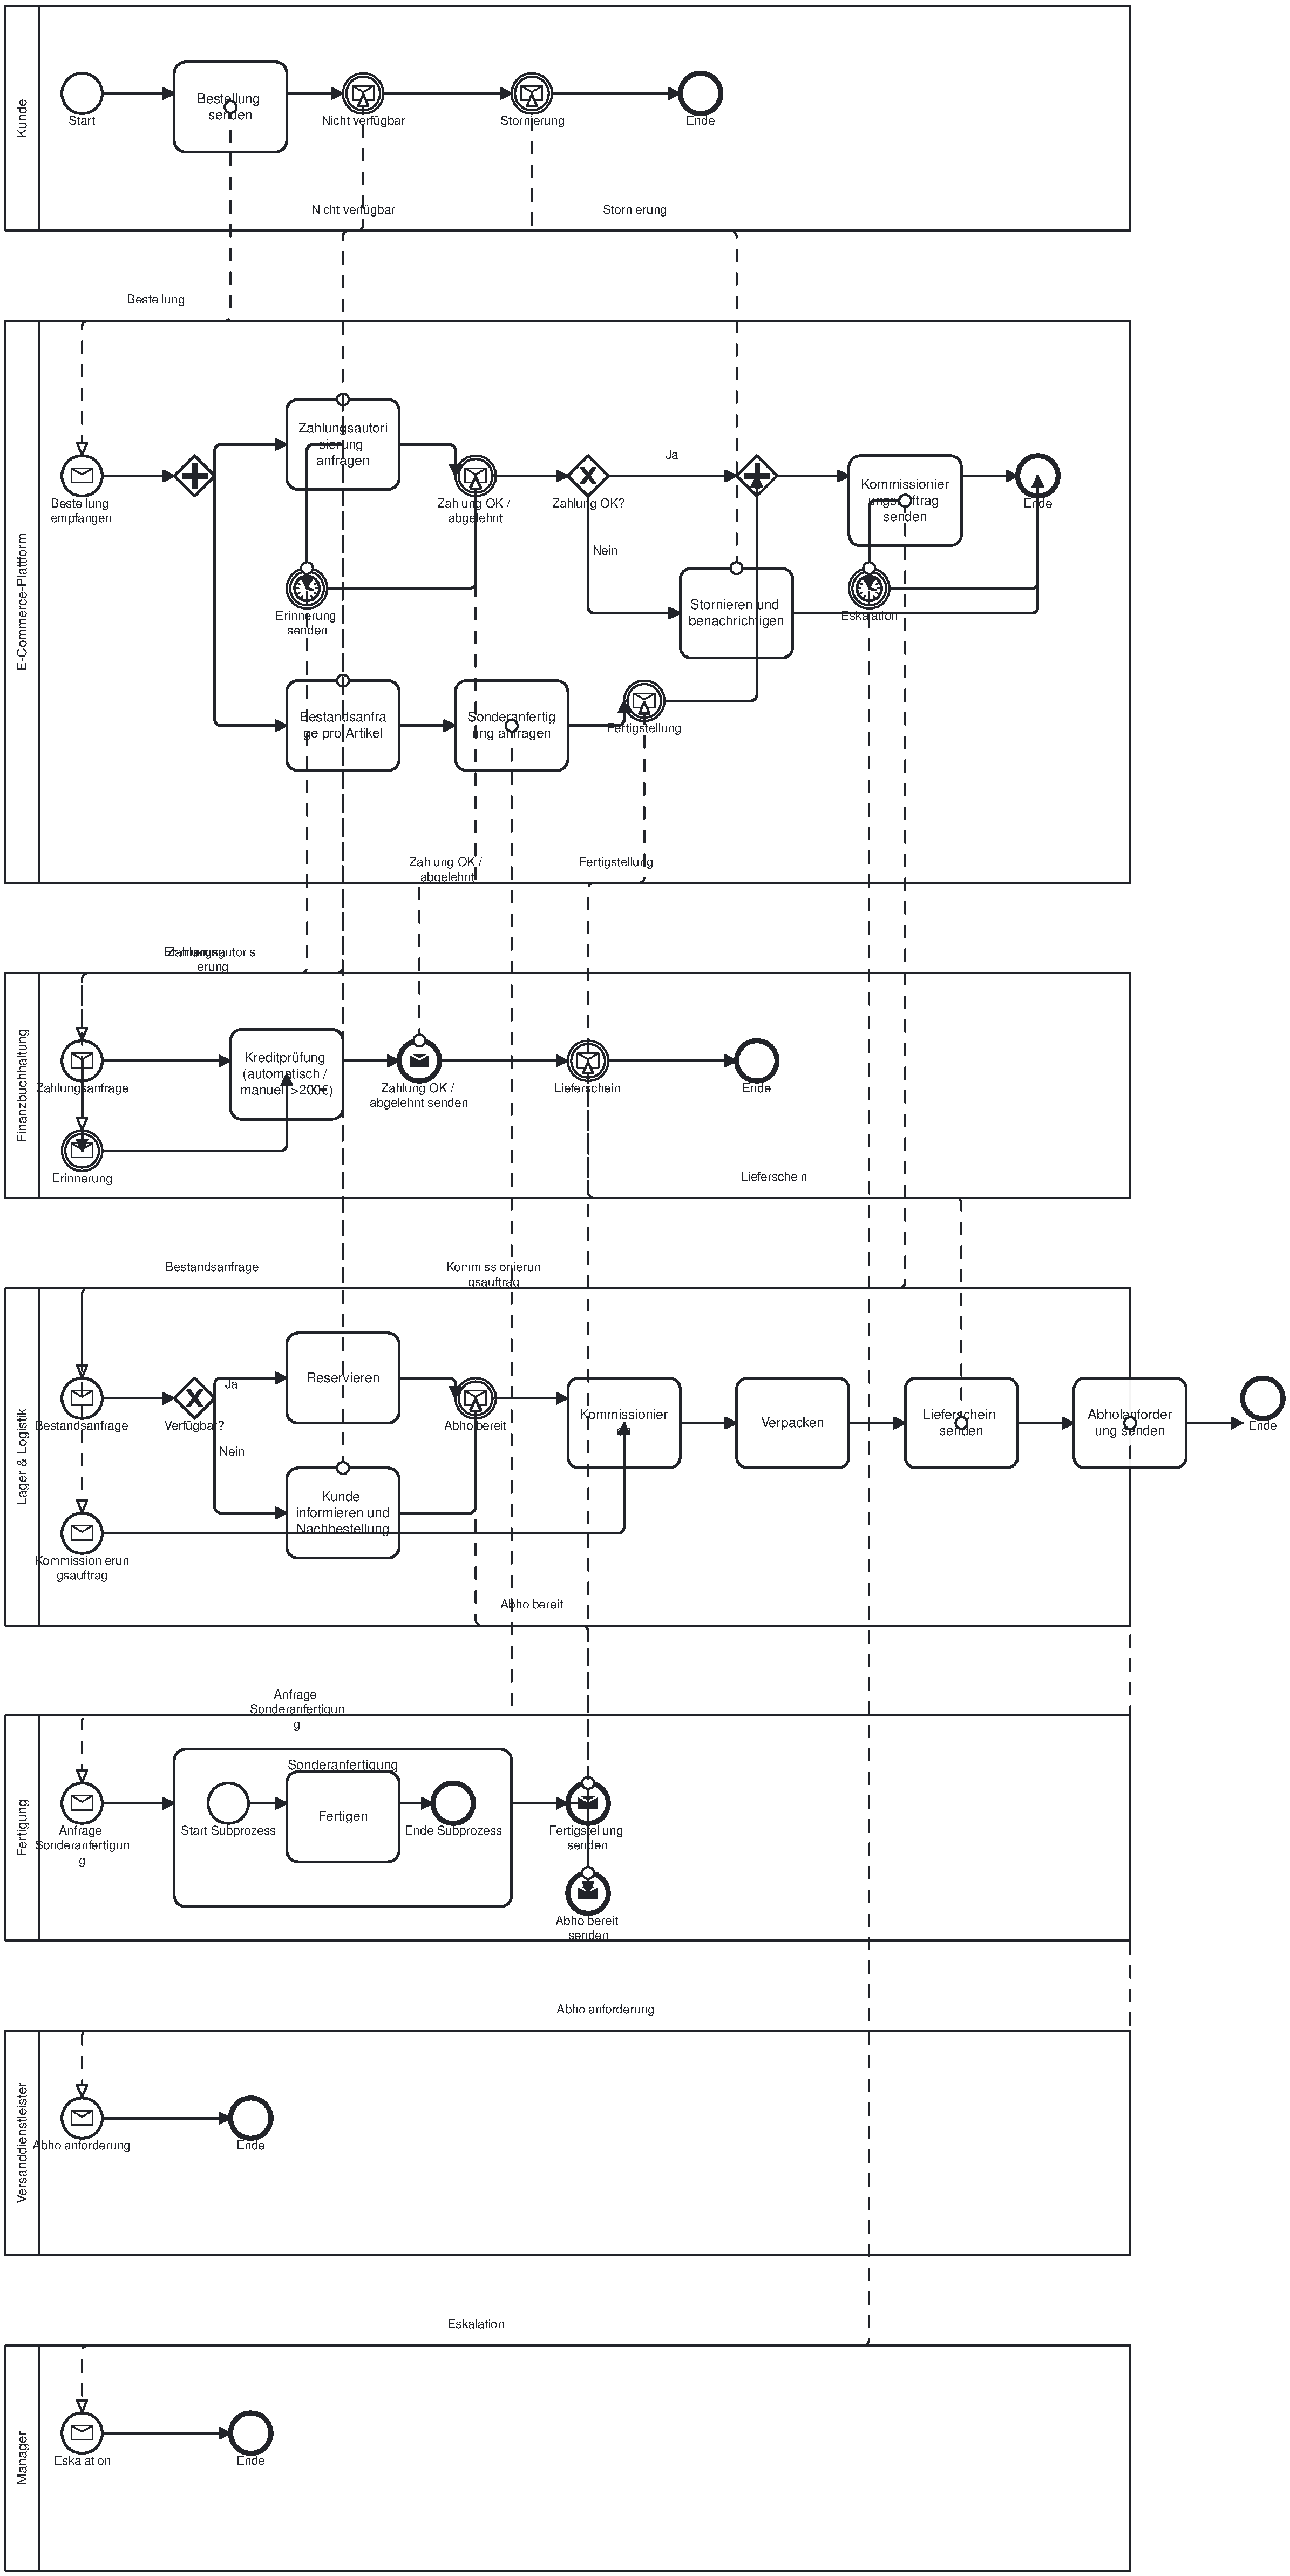
\includegraphics[height=.9\textheight]{images/diagrams/grok-4-(xml)-o3fefday}
  \caption{Diagramm von Grok 4 mit XML \\ 13268 TOKEN | 0.250 \$ | 604 s}
  \label{fig:grok-4-xml}
\end{figure}

\begin{figure}[!htb]
  \centering
  \includegraphics[width=\textwidth]{images/diagrams/grok-4-1-fast-reasoning-(json)-udjbgpm1}
  \caption{Diagramm von Grok 4.1 Fast mit JSON \\ 9640 TOKEN | 0.015 \$ | 191 s}
  \label{fig:grok-4-1-json}
\end{figure}

\begin{figure}[!htb]
  \centering
  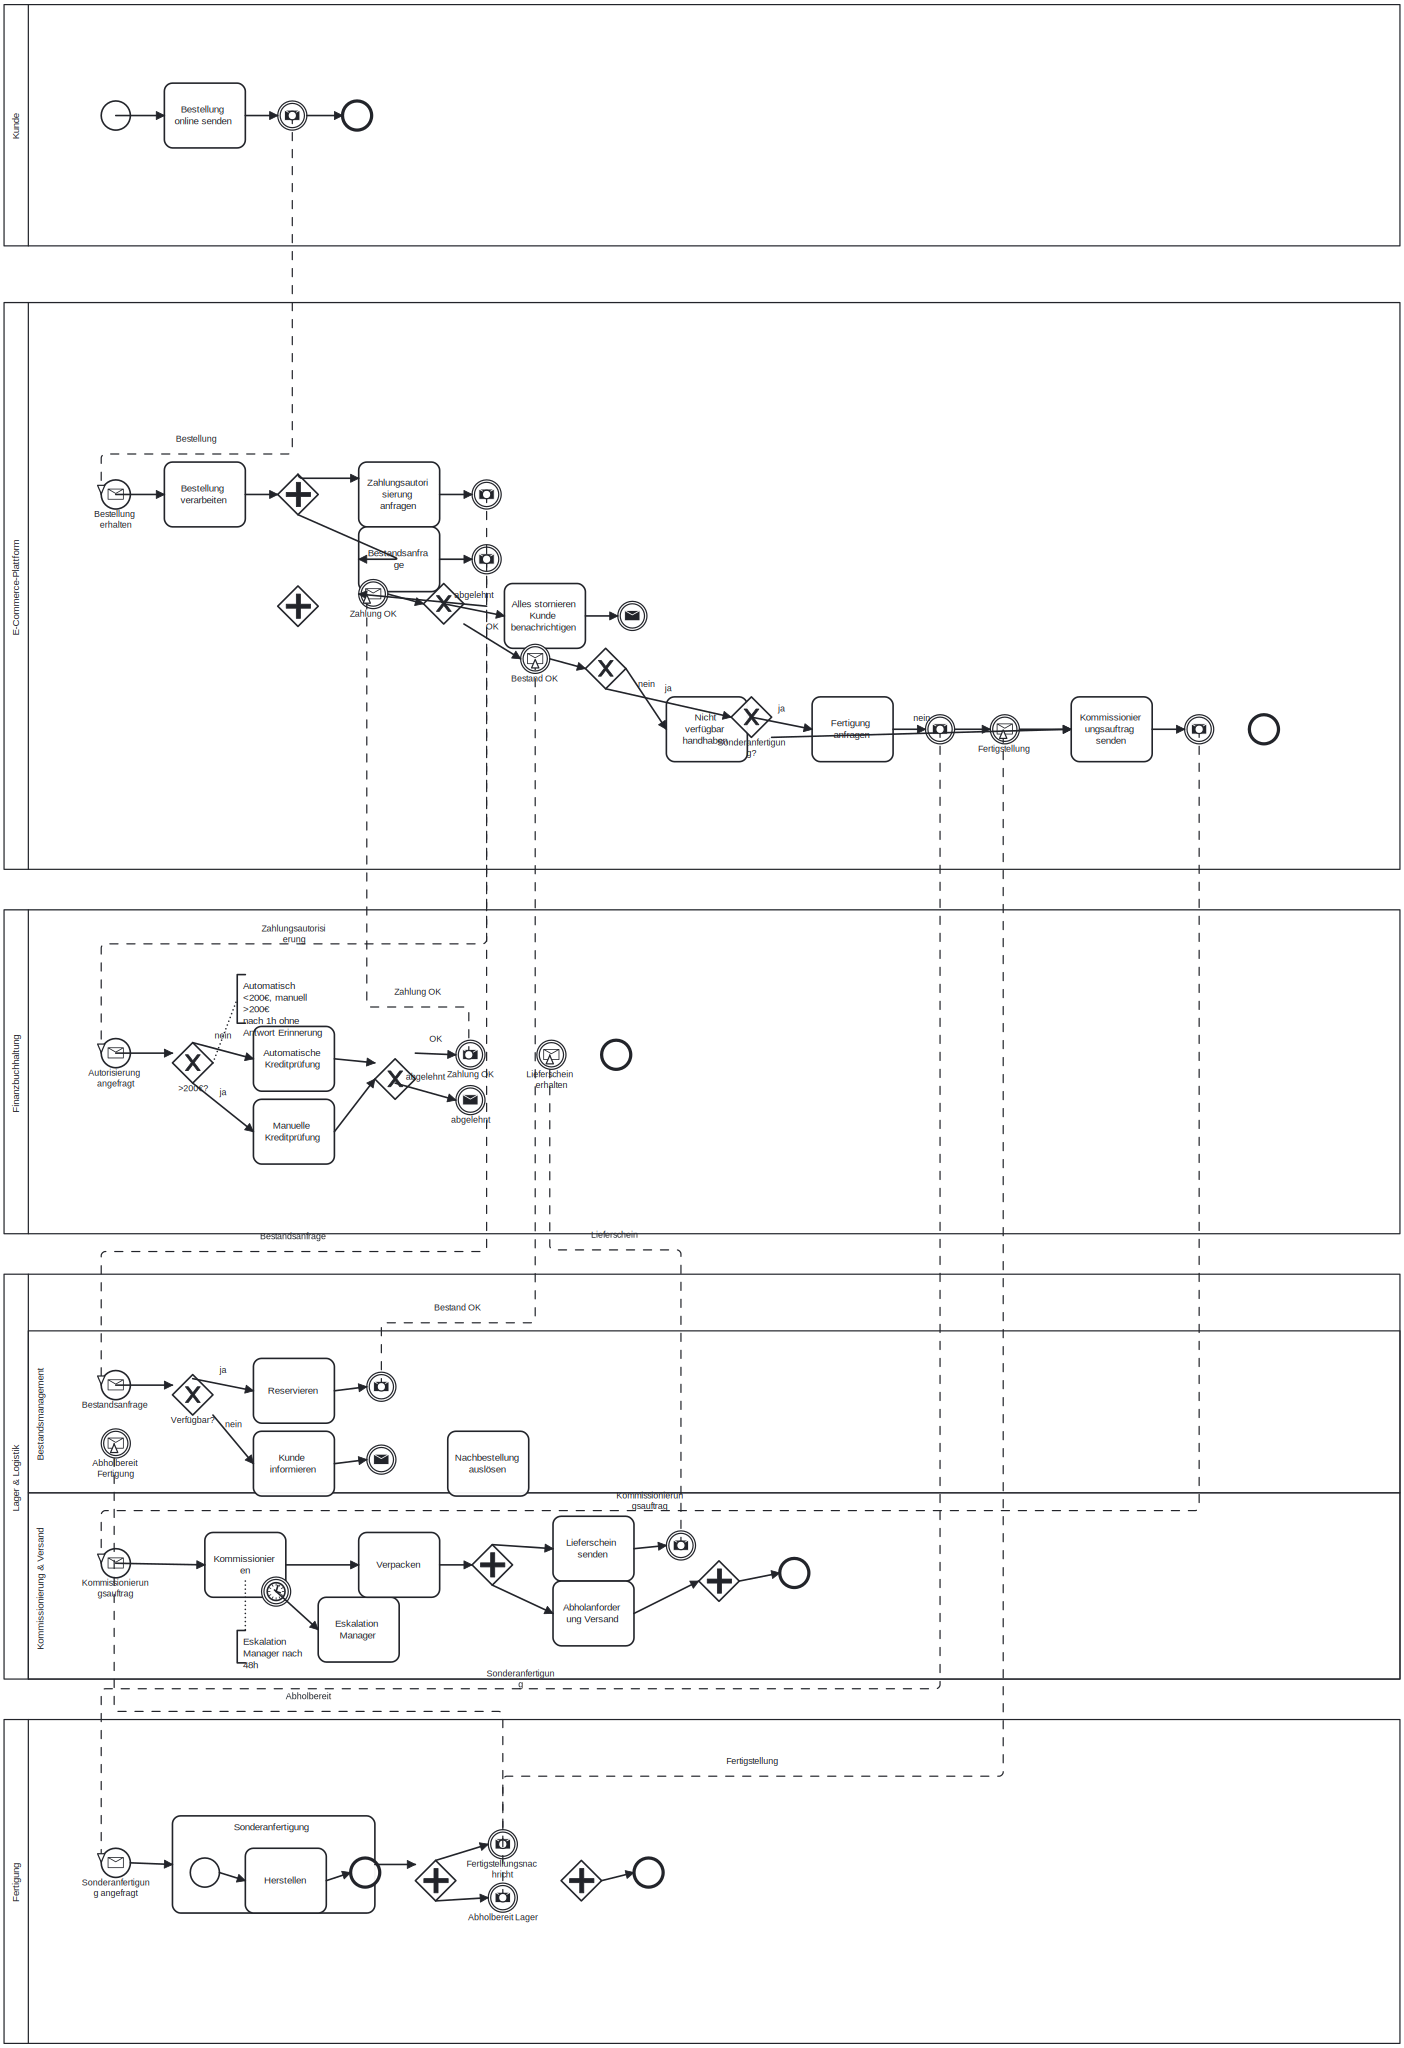
\includegraphics[height=.9\textheight]{images/diagrams/grok-4-1-fast-reasoning-(xml)-c0ivs3u9}
  \caption{Diagramm von Grok 4.1 Fast mit XML \\ 16555 TOKEN | 0.016 \$ | 200 s}
  \label{fig:grok-4-1-xml}
\end{figure}

\begin{figure}[!htb]
  \centering
  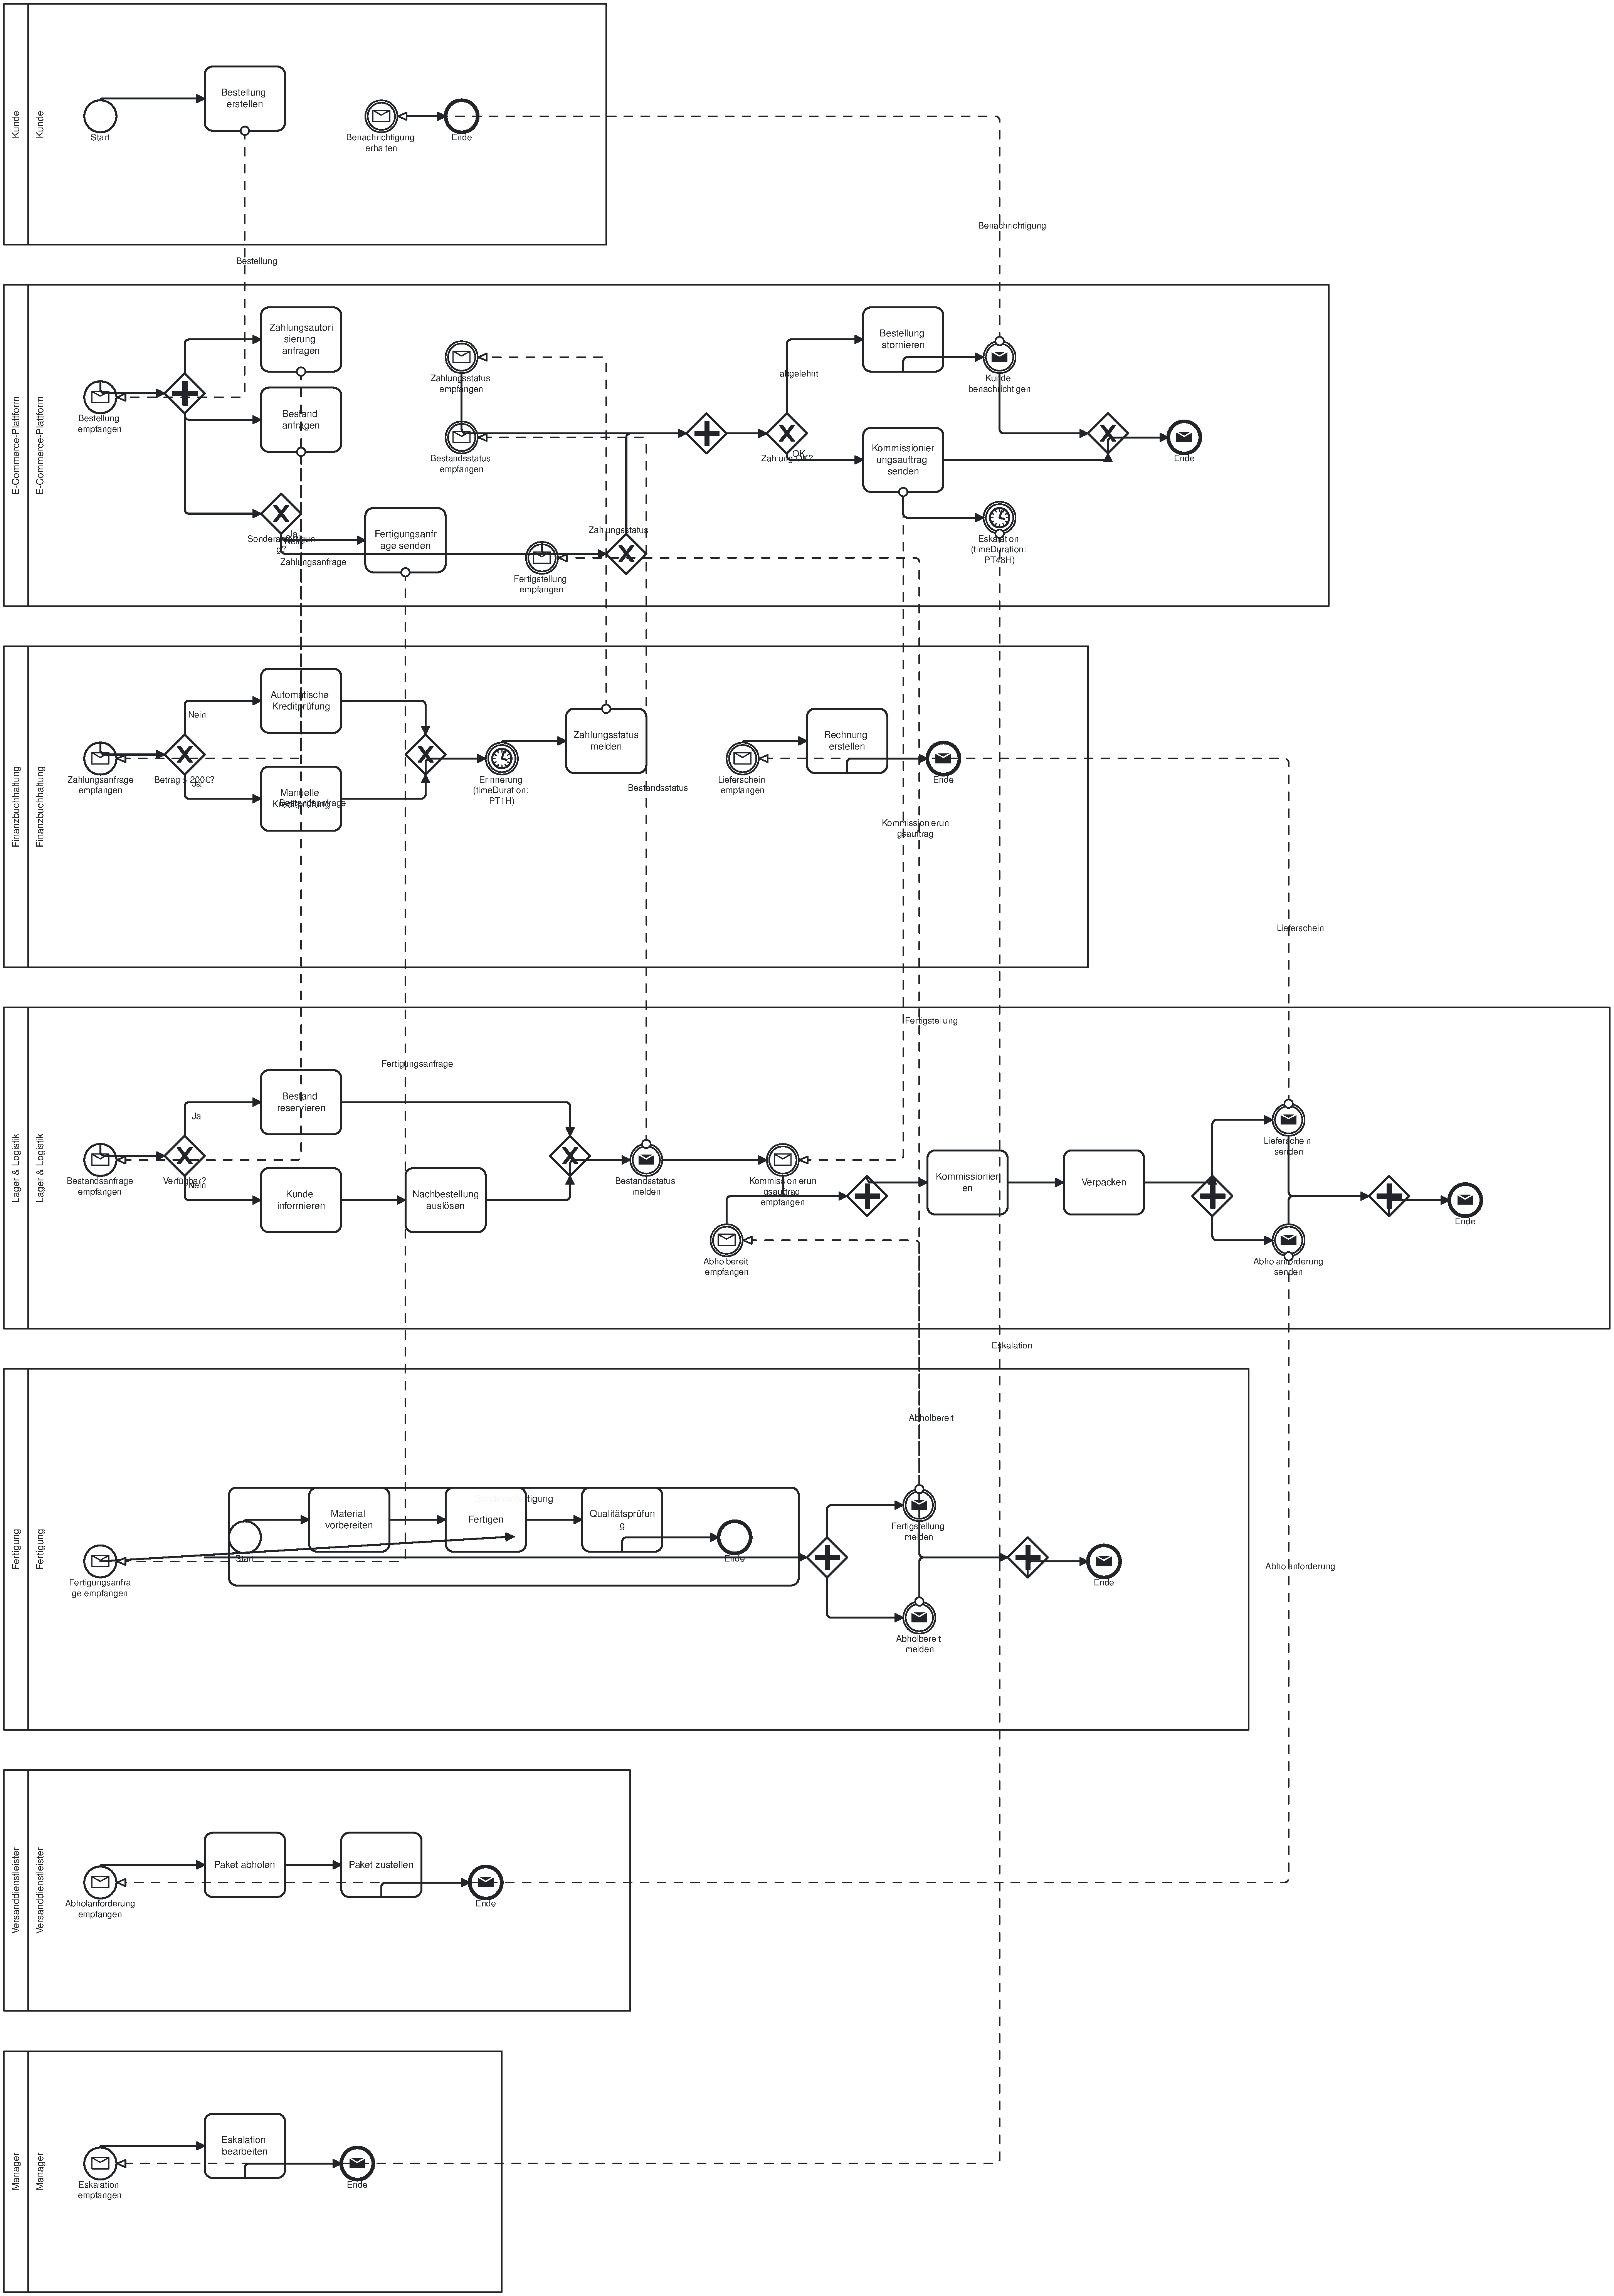
\includegraphics[height=.9\textheight]{images/diagrams/claude-opus-4-5-(json)-wkq3inzs}
  \caption{Diagramm von Claude Opus 4.5 mit JSON \\ 13826 TOKEN | 0.421 \$ | 118 s}
  \label{fig:claude-opus-4-5-json}
\end{figure}

\begin{figure}[!htb]
  \centering
  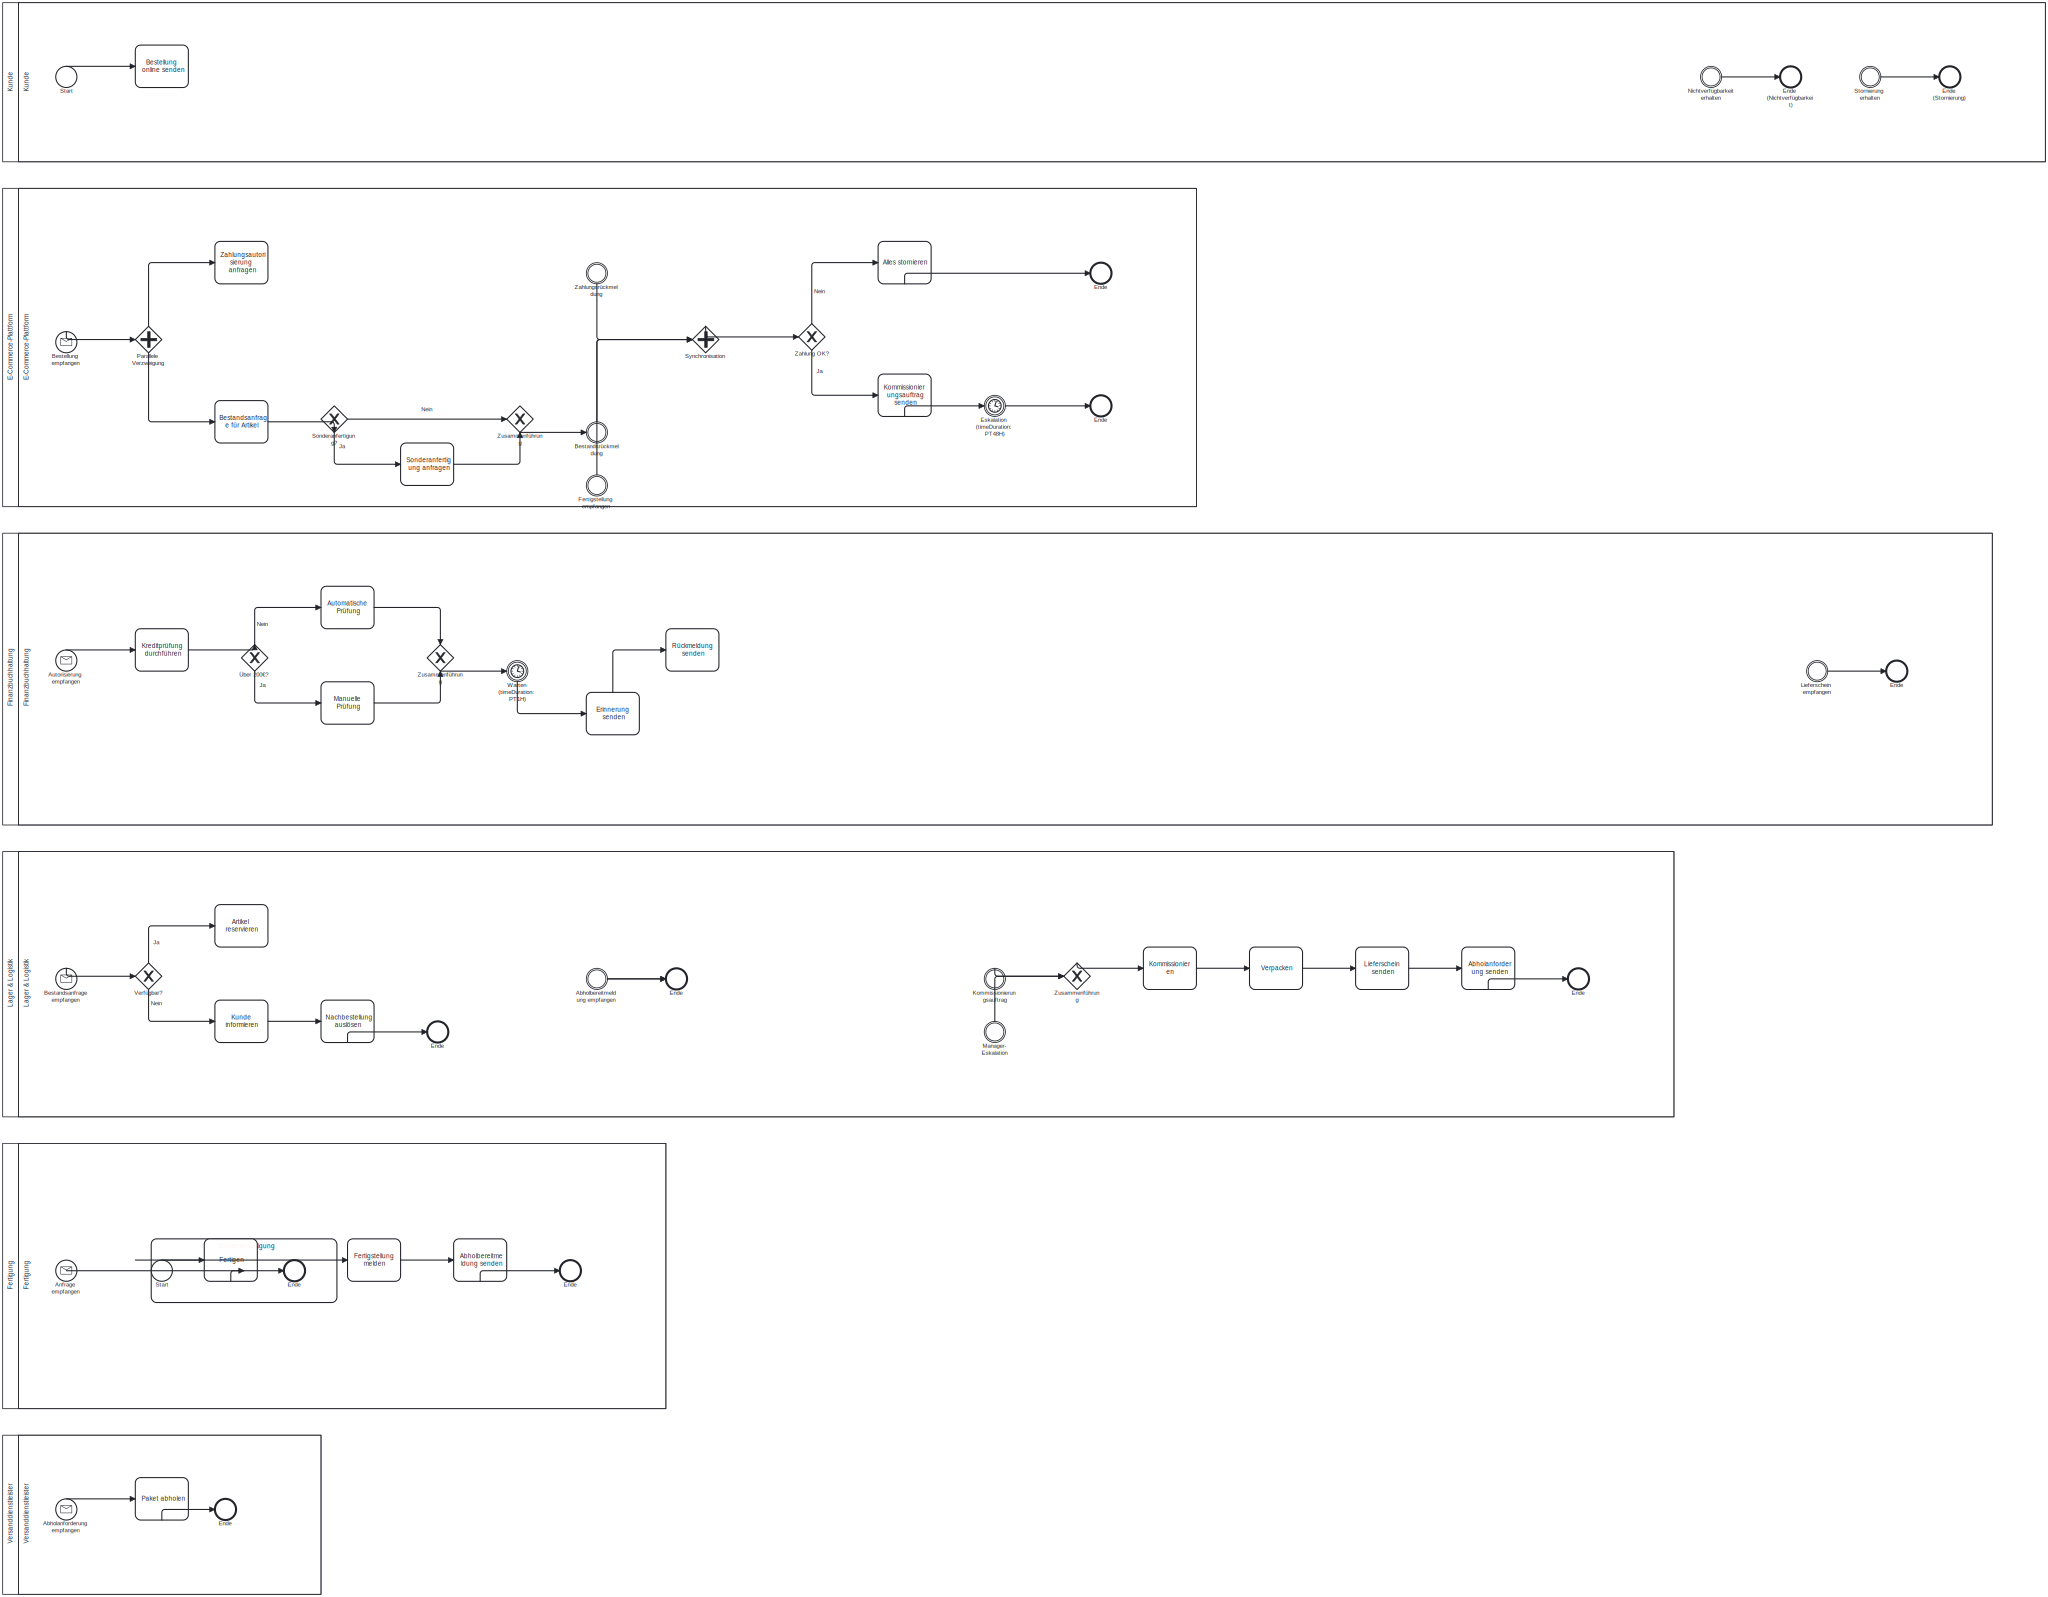
\includegraphics[width=\textwidth]{images/diagrams/claude-sonnet-4-5-(json)-hy0axos0}
  \caption{Diagramm von Claude Sonnet 4.5 mit JSON \\ 11172 TOKEN | 0.213 \$ | 107 s}
  \label{fig:claude-sonnet-4-5-json}
\end{figure}

\begin{figure}[!htb]
  \centering
  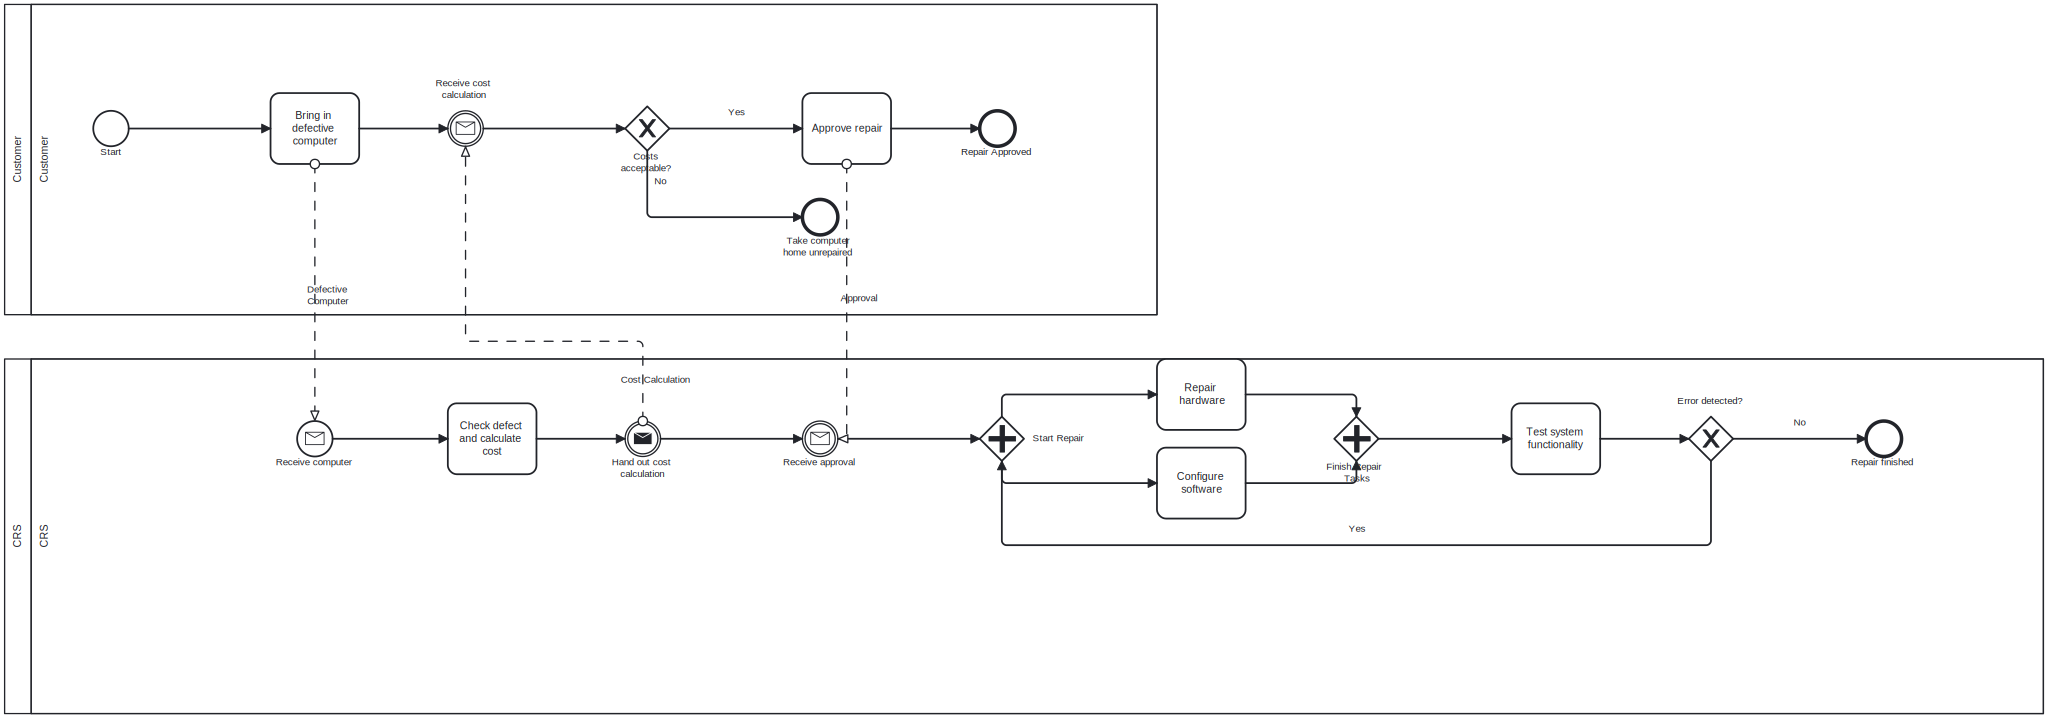
\includegraphics[width=\textwidth]{images/diagrams/gemini-2.5-pro-(json)-q39fumx1}
  \caption{Diagramm von Gemini 2.5 Pro mit JSON \\ 3817 TOKEN | 0.000 \$ | 63 s}
  \label{fig:gemini-2-5-pro-json-2}
\end{figure}

\begin{figure}[!htb]
  \centering
  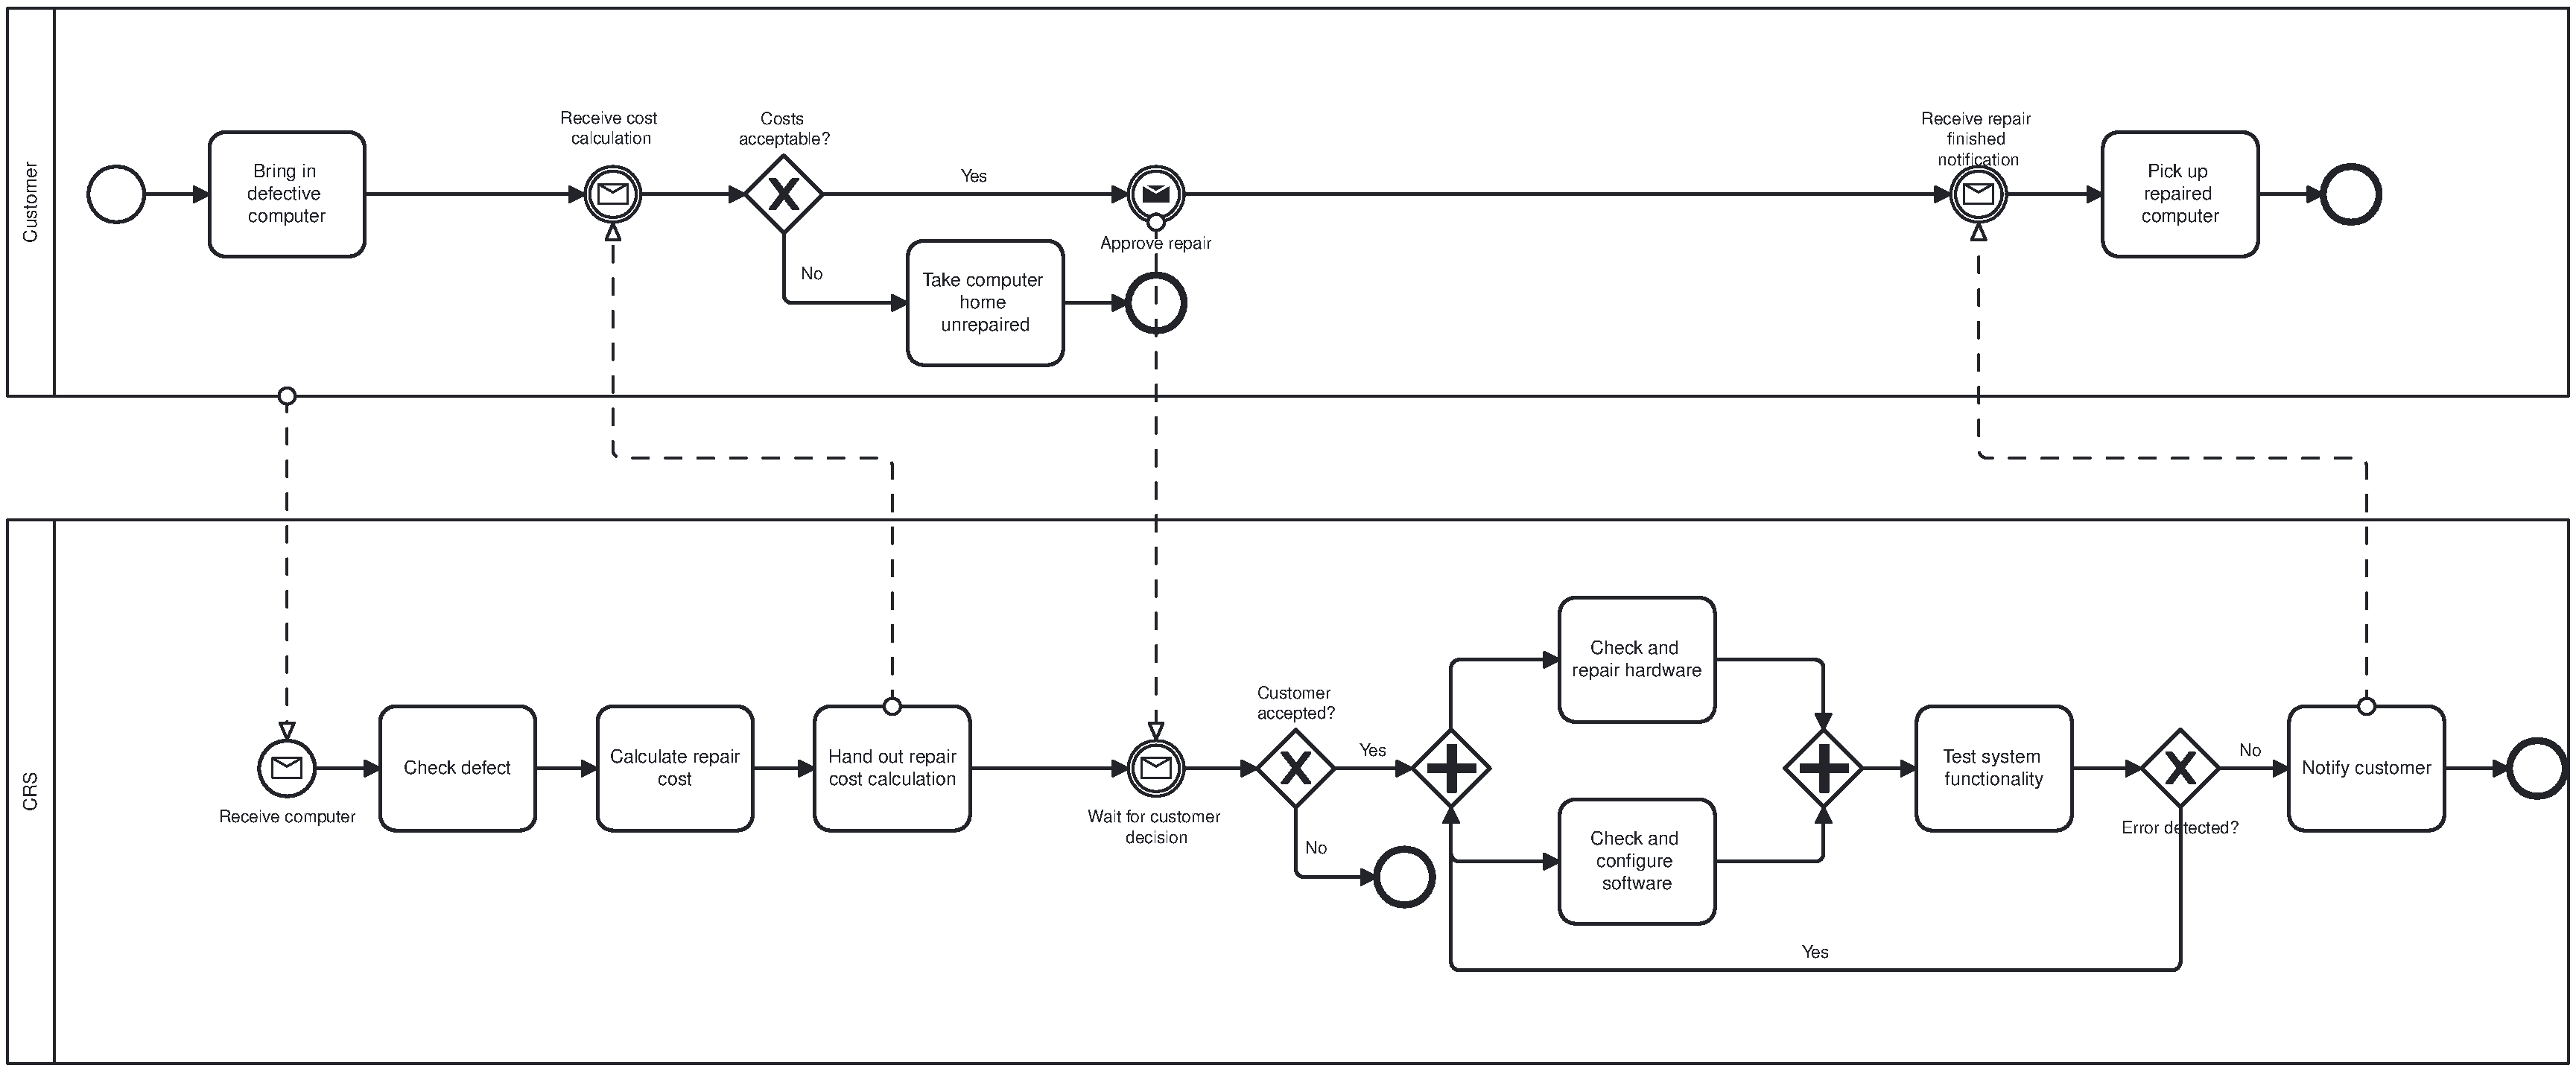
\includegraphics[width=\textwidth]{images/diagrams/gemini-2.5-pro-(xml)-k2oeauto}
  \caption{Diagramm von Gemini 2.5 Pro mit XML\\ 8632 TOKEN | 0.000 \$ | 94 s}
  \label{fig:gemini-2-5-pro-xml-2}
\end{figure}

\begin{figure}[!htb]
  \centering
  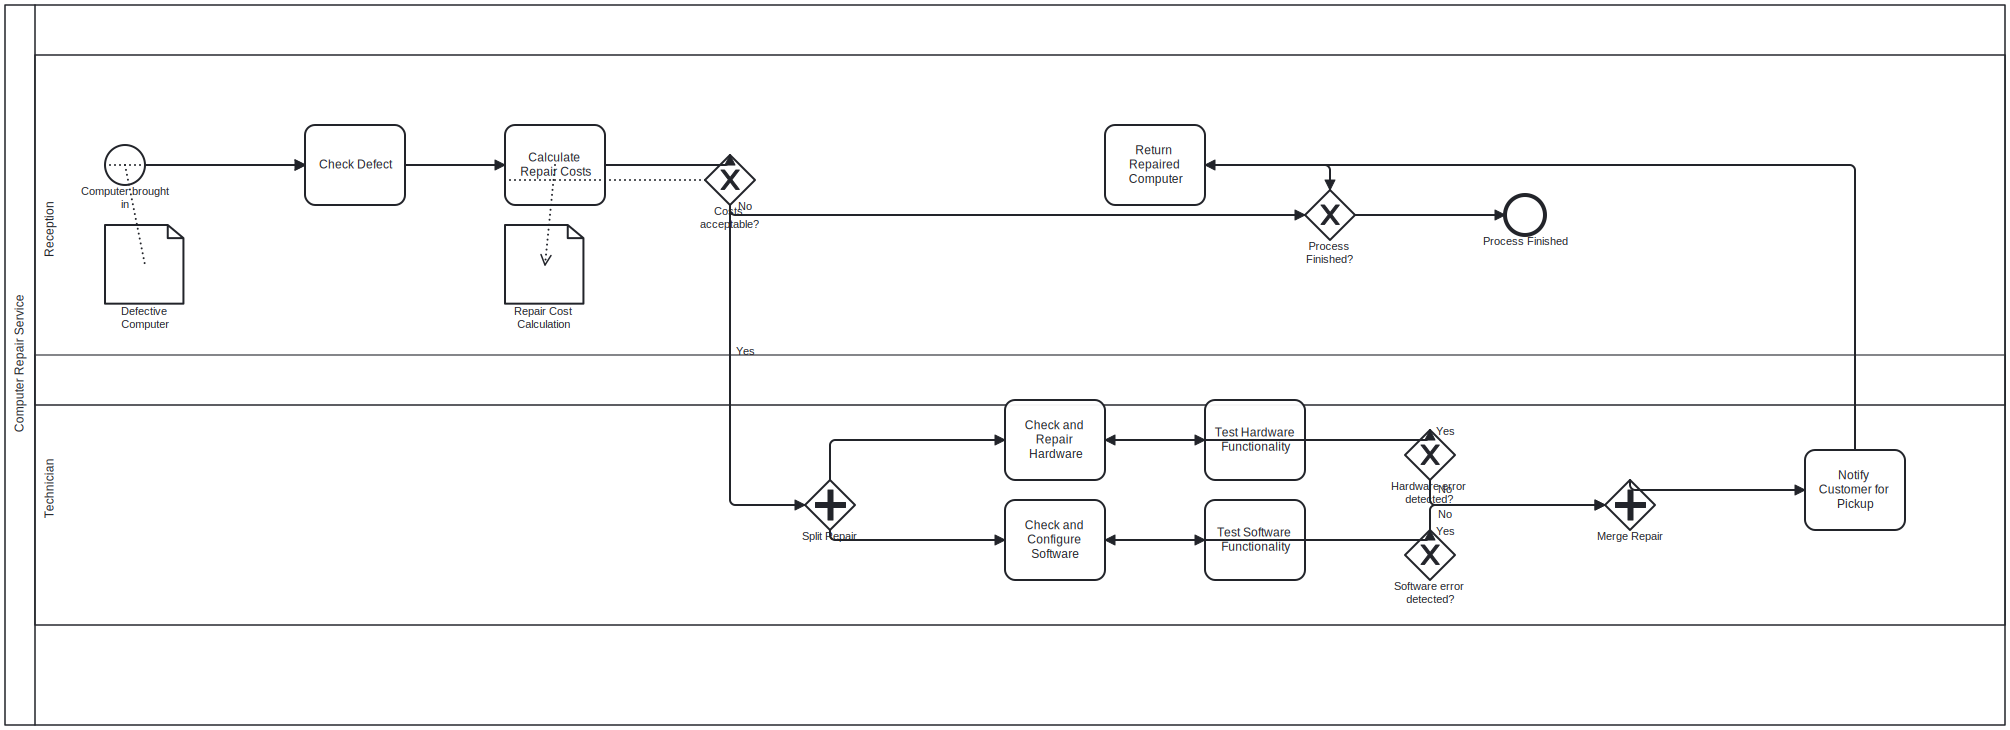
\includegraphics[width=\textwidth]{images/diagrams/gemini-2.5-flash-(json)-7w0r7fdv}
  \caption{Diagramm von Gemini 2.5 Flash mit JSON \\ 3938 TOKEN | 0.000 \$ | 95 s}
  \label{fig:gemini-2-5-flash-json-2}
\end{figure}

\begin{figure}[!htb]
  \centering
  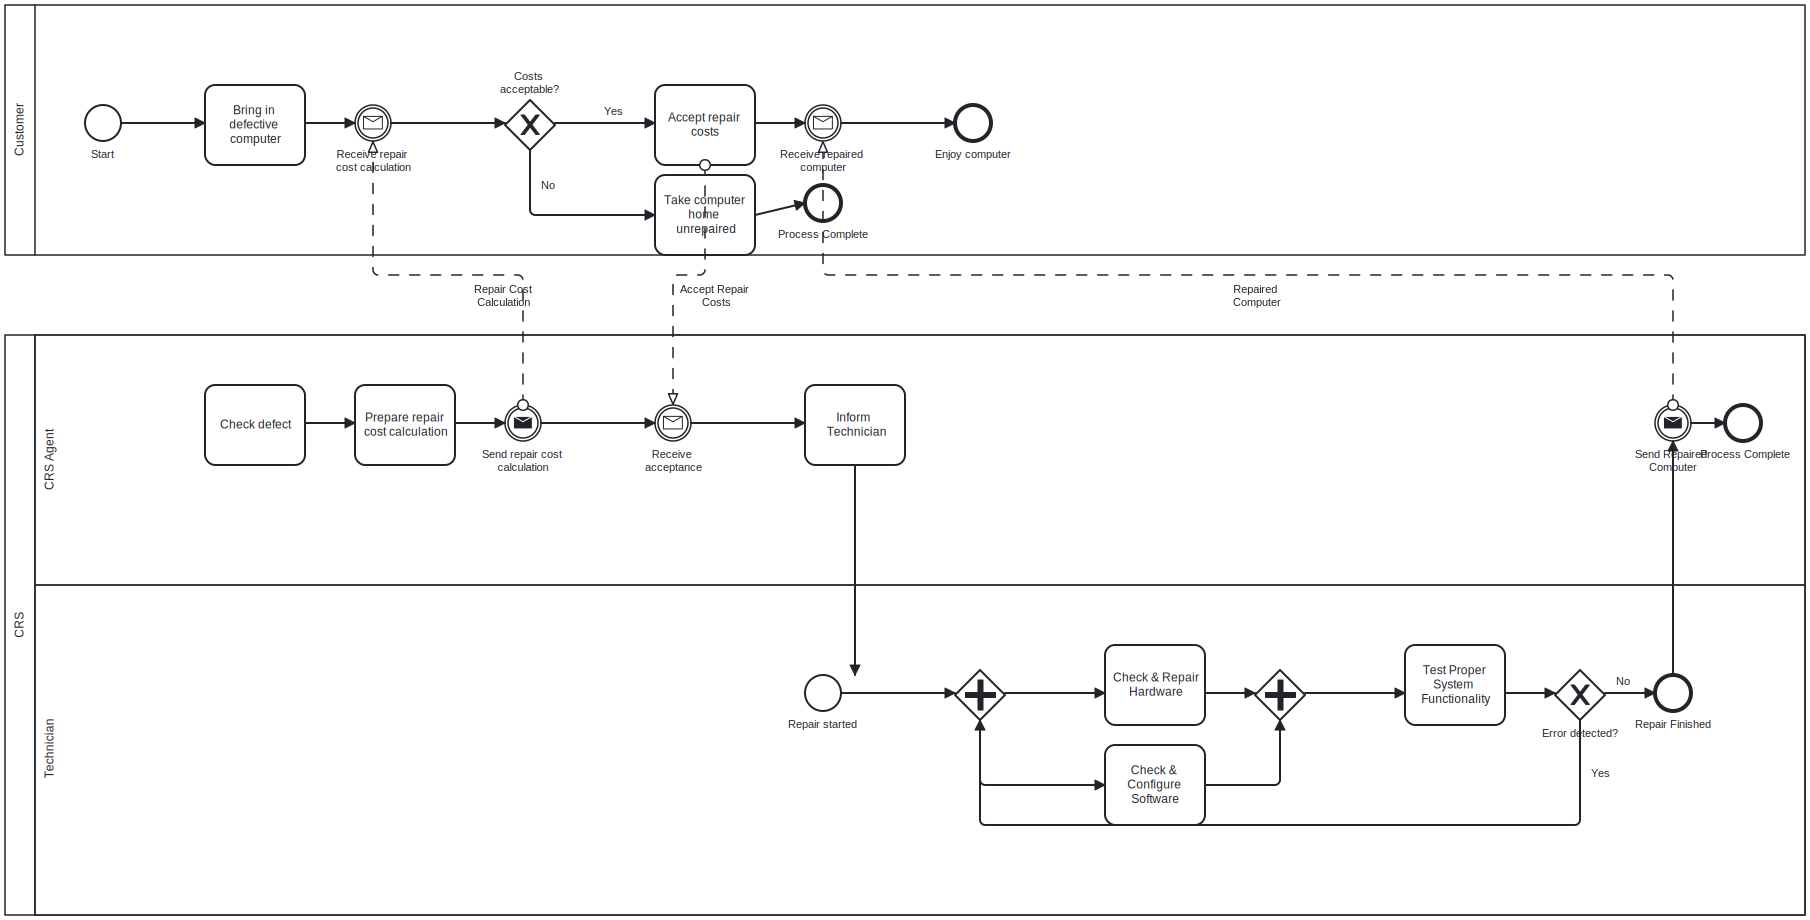
\includegraphics[width=\textwidth]{images/diagrams/gemini-2.5-flash-(xml)-t0pflpsy}
  \caption{Diagramm von Gemini 2.5 Flash mit XML \\ 10757 TOKEN | 0.000 \$ | 84 s}
  \label{fig:gemini-2-5-flash-xml-2}
\end{figure}

\begin{figure}[!htb]
  \centering
  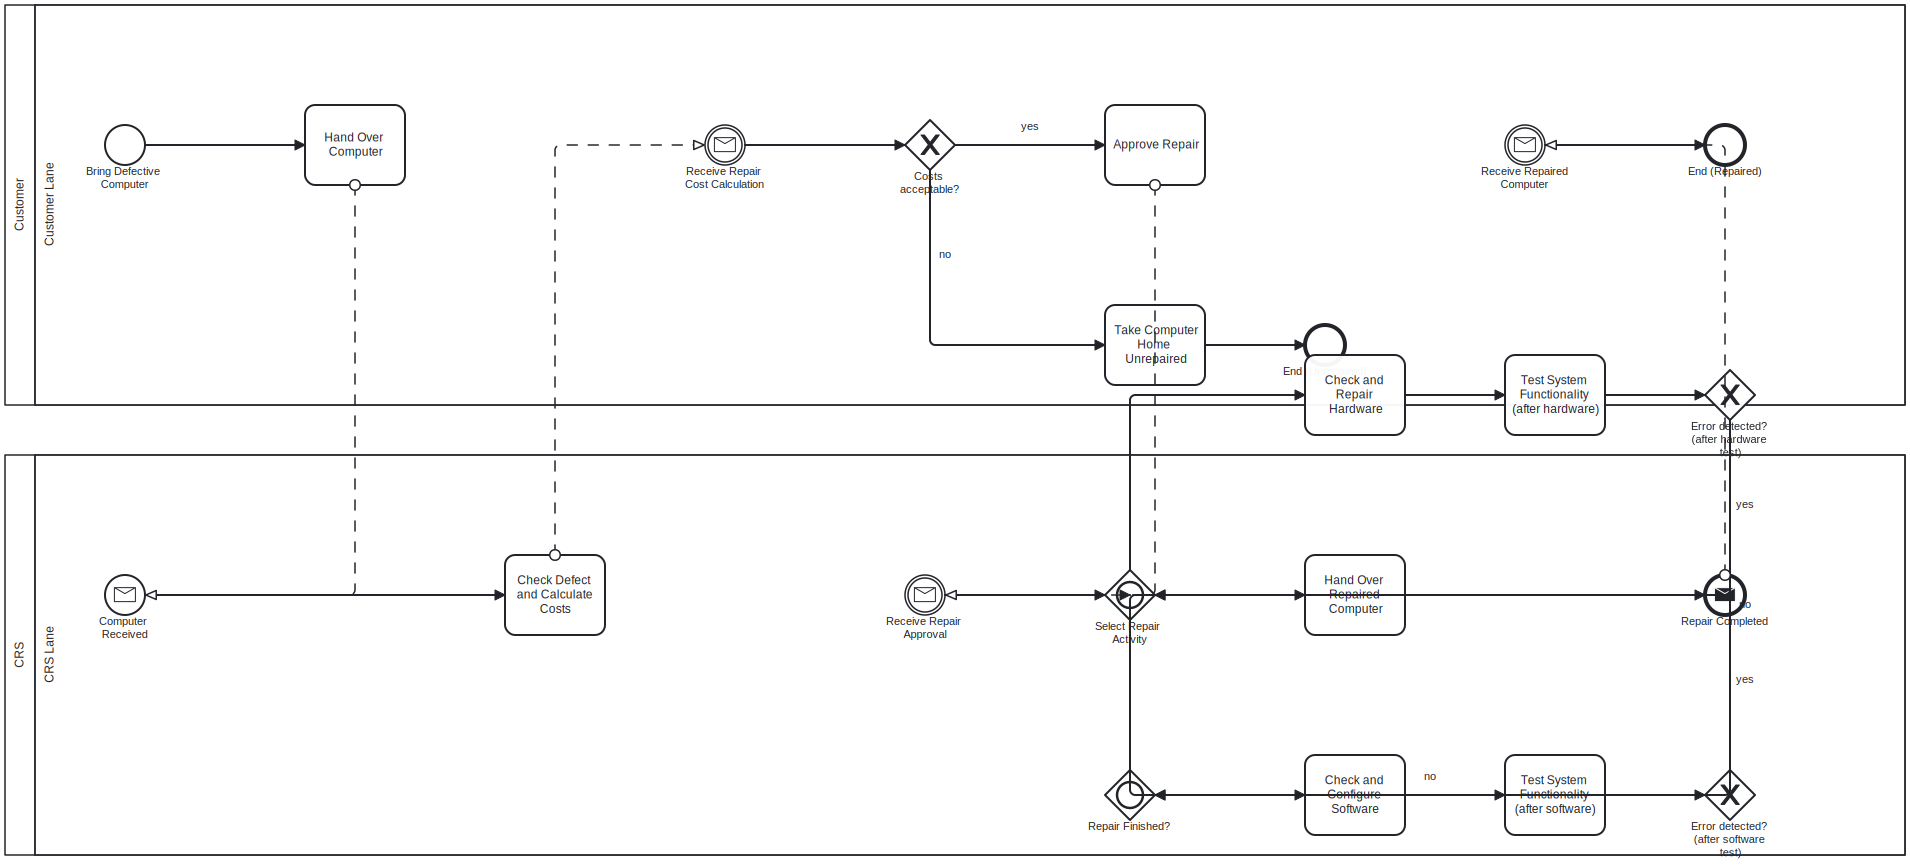
\includegraphics[width=\textwidth]{images/diagrams/gpt-5.2-(json)-qwz0g28q}
  \caption{Diagramm von ChatGPT 5.2 mit JSON \\ 3651 TOKEN | 0.072 \$ | 27 s}
  \label{fig:gpt-5-2-json-2}
\end{figure}

\begin{figure}[!htb]
  \centering
  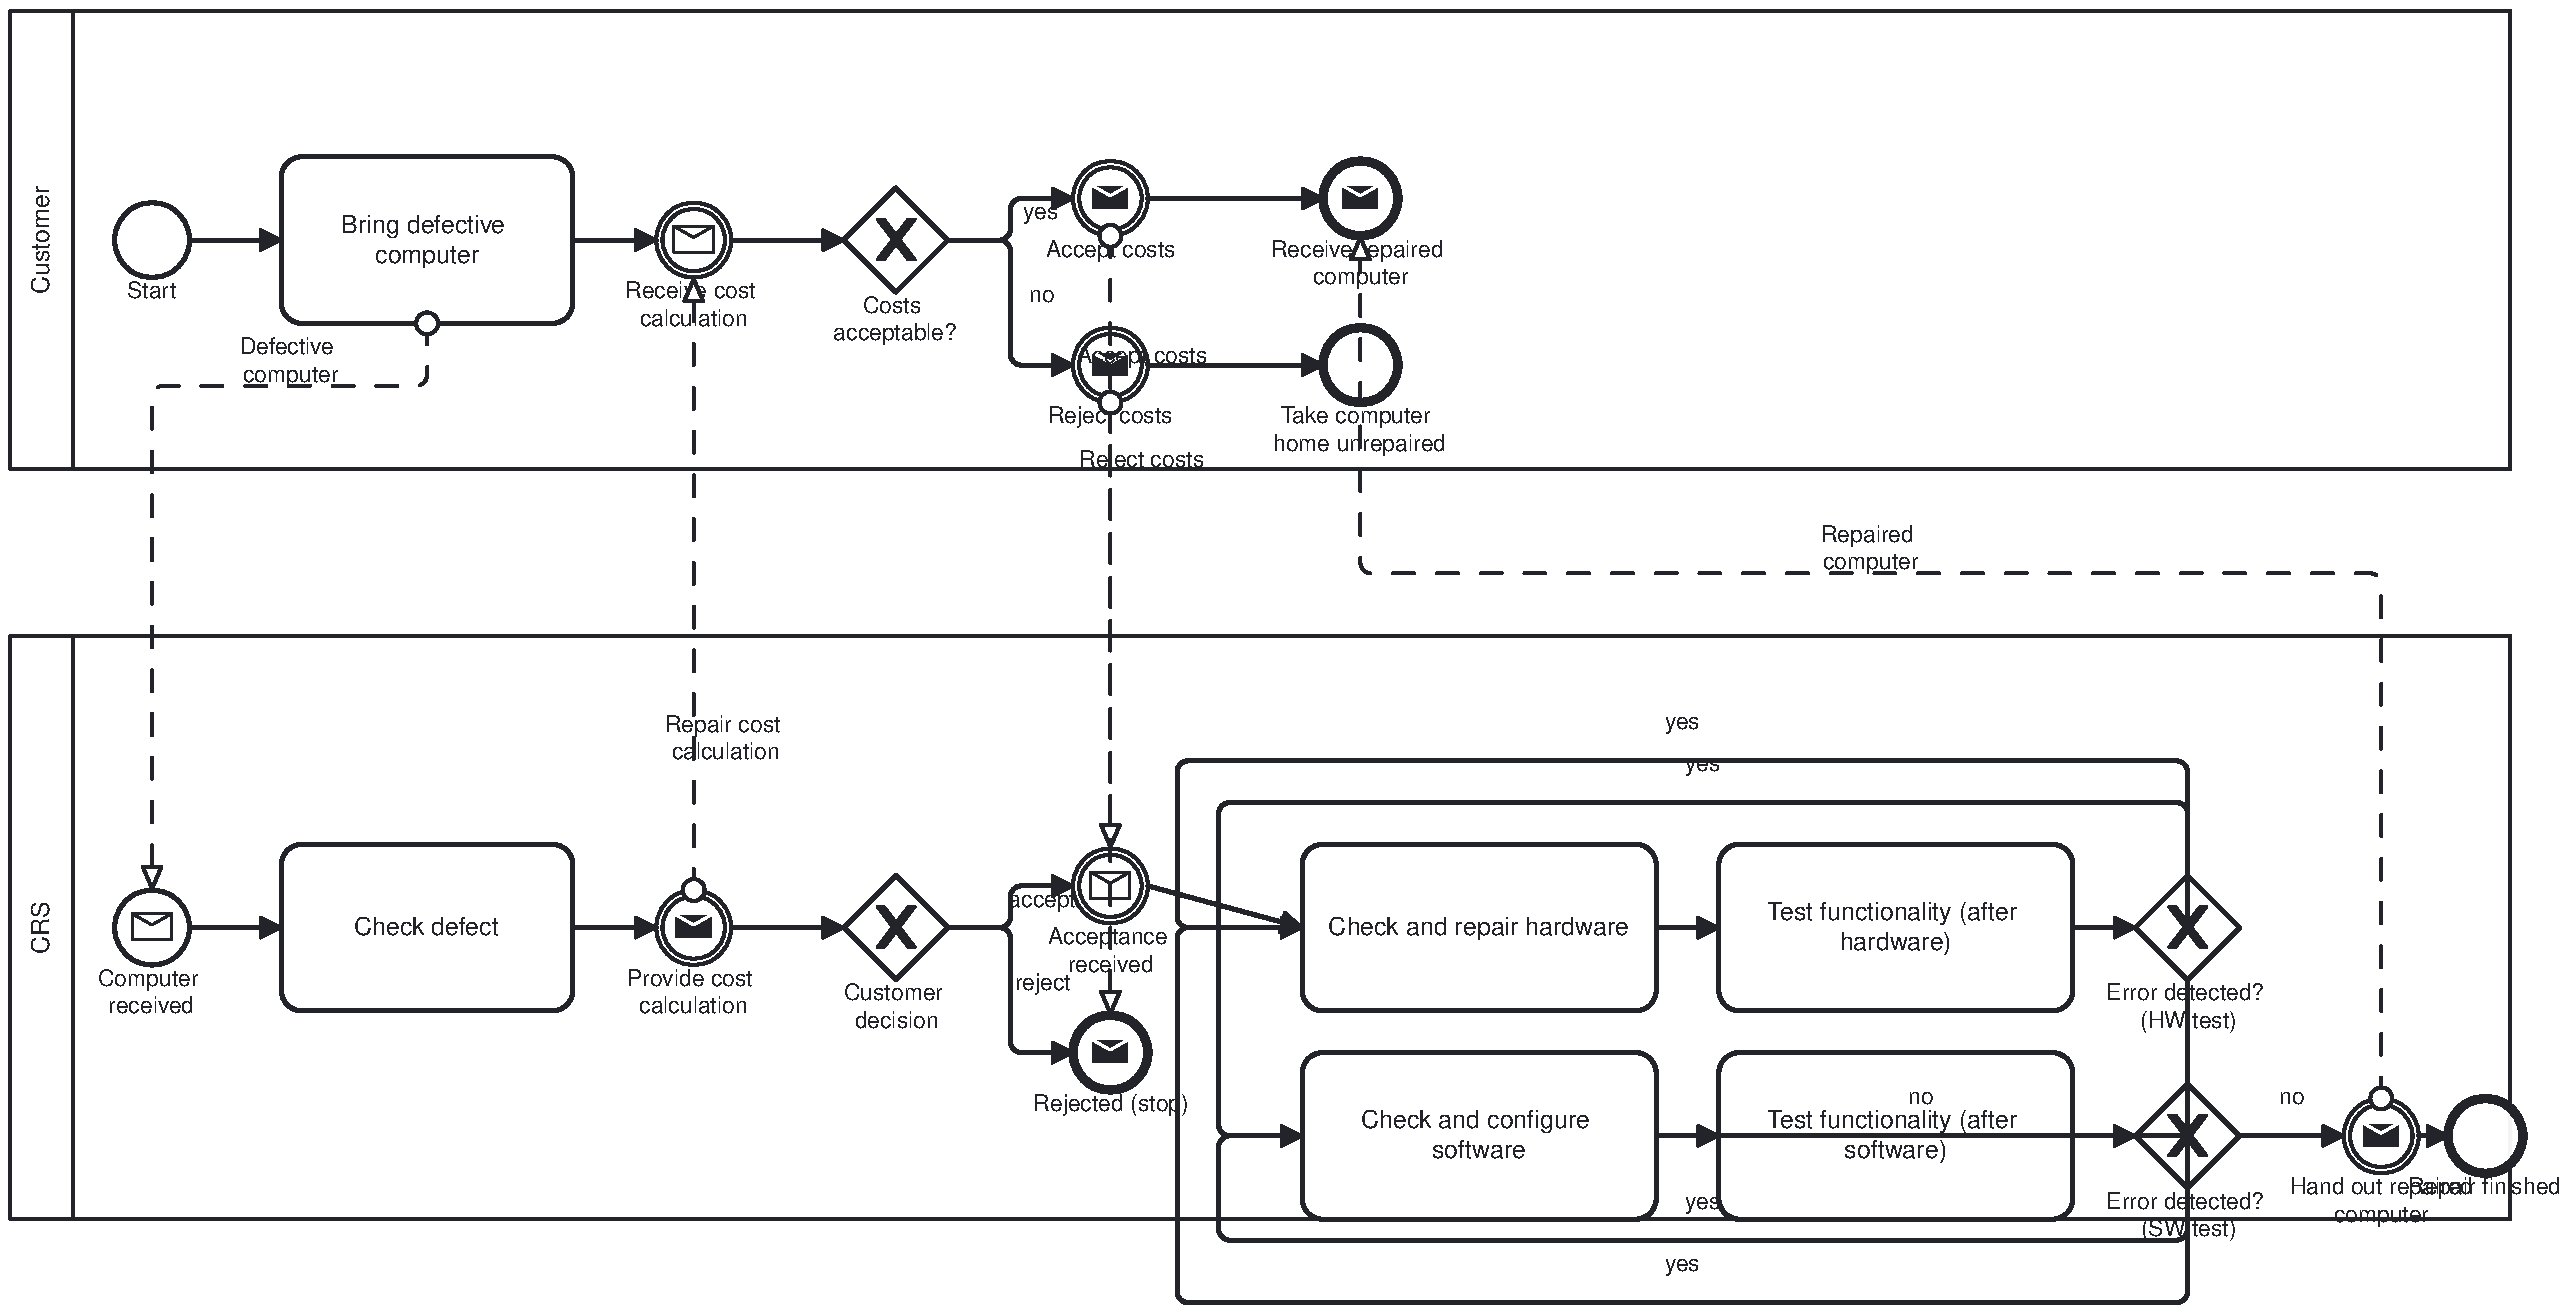
\includegraphics[width=\textwidth]{images/diagrams/gpt-5.2-(xml)-vg5j1d7k}
  \caption{Diagramm von ChatGPT 5.2 mit XML \\ 6767 TOKEN | 0.118 \$ | 50 s}
  \label{fig:gpt-5-2-xml-2}
\end{figure}

\begin{figure}[!htb]
  \centering
  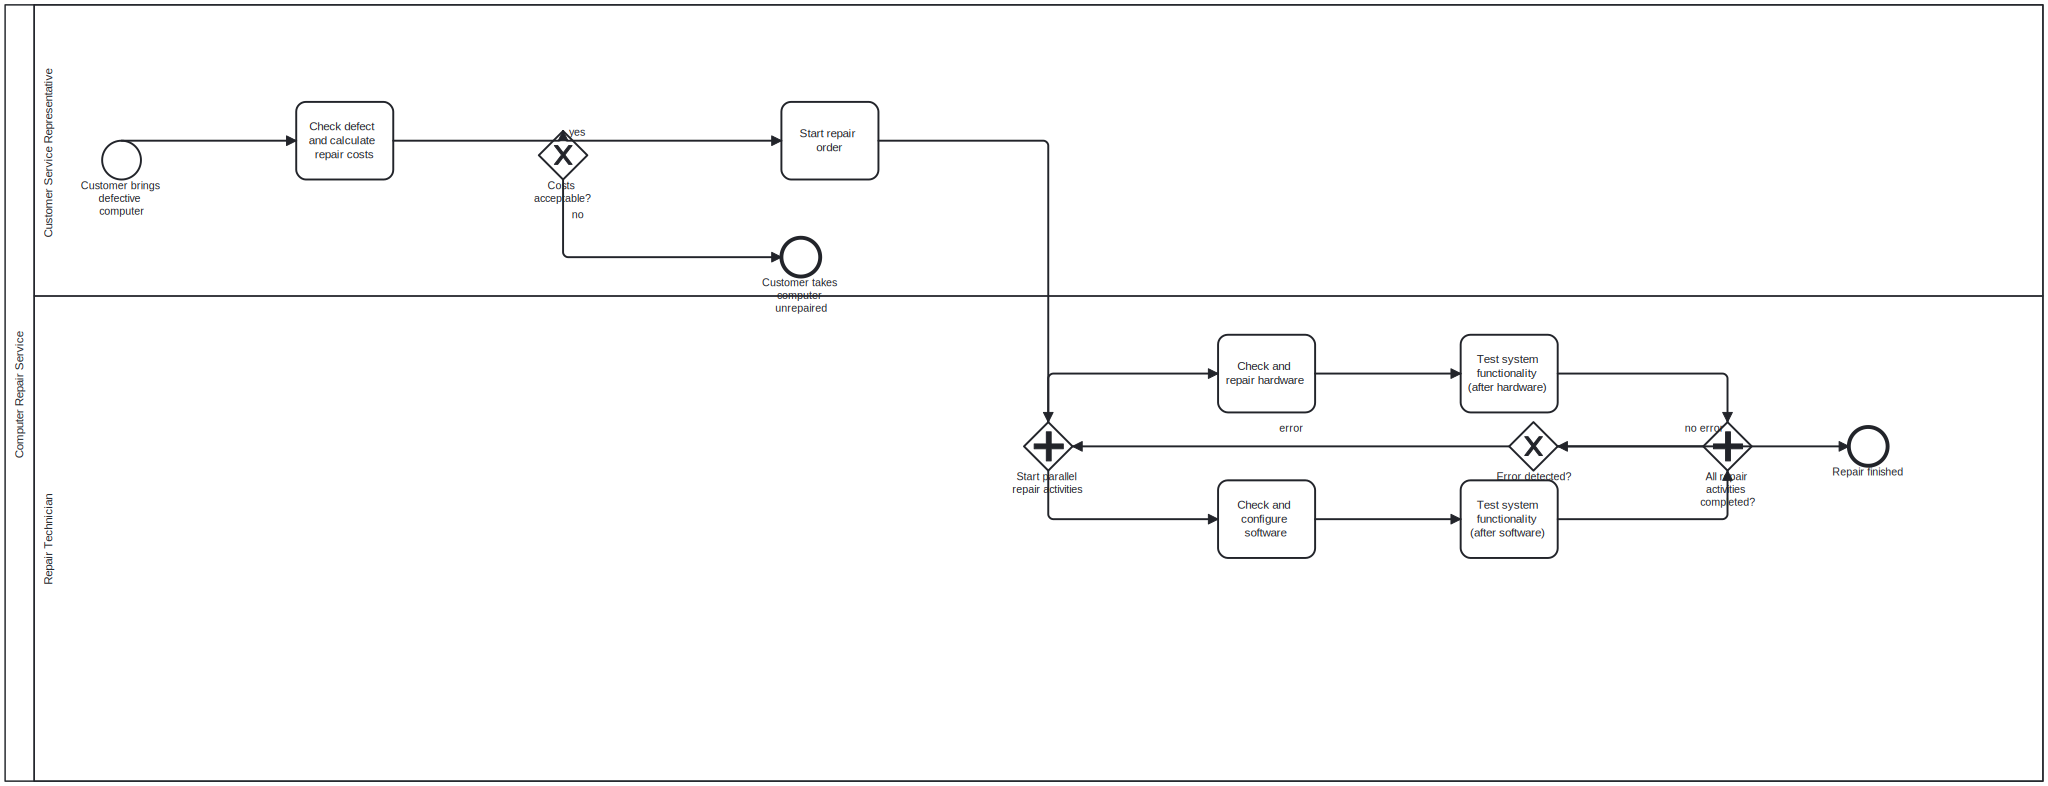
\includegraphics[width=\textwidth]{images/diagrams/gpt-5.1-(json)-duk2bj46}
  \caption{Diagramm von ChatGPT 5.1 mit JSON \\ 1895 TOKEN | 0.034 \$ | 22 s}
  \label{fig:gpt-5-1-json-2}
\end{figure}

\begin{figure}[!htb]
  \centering
  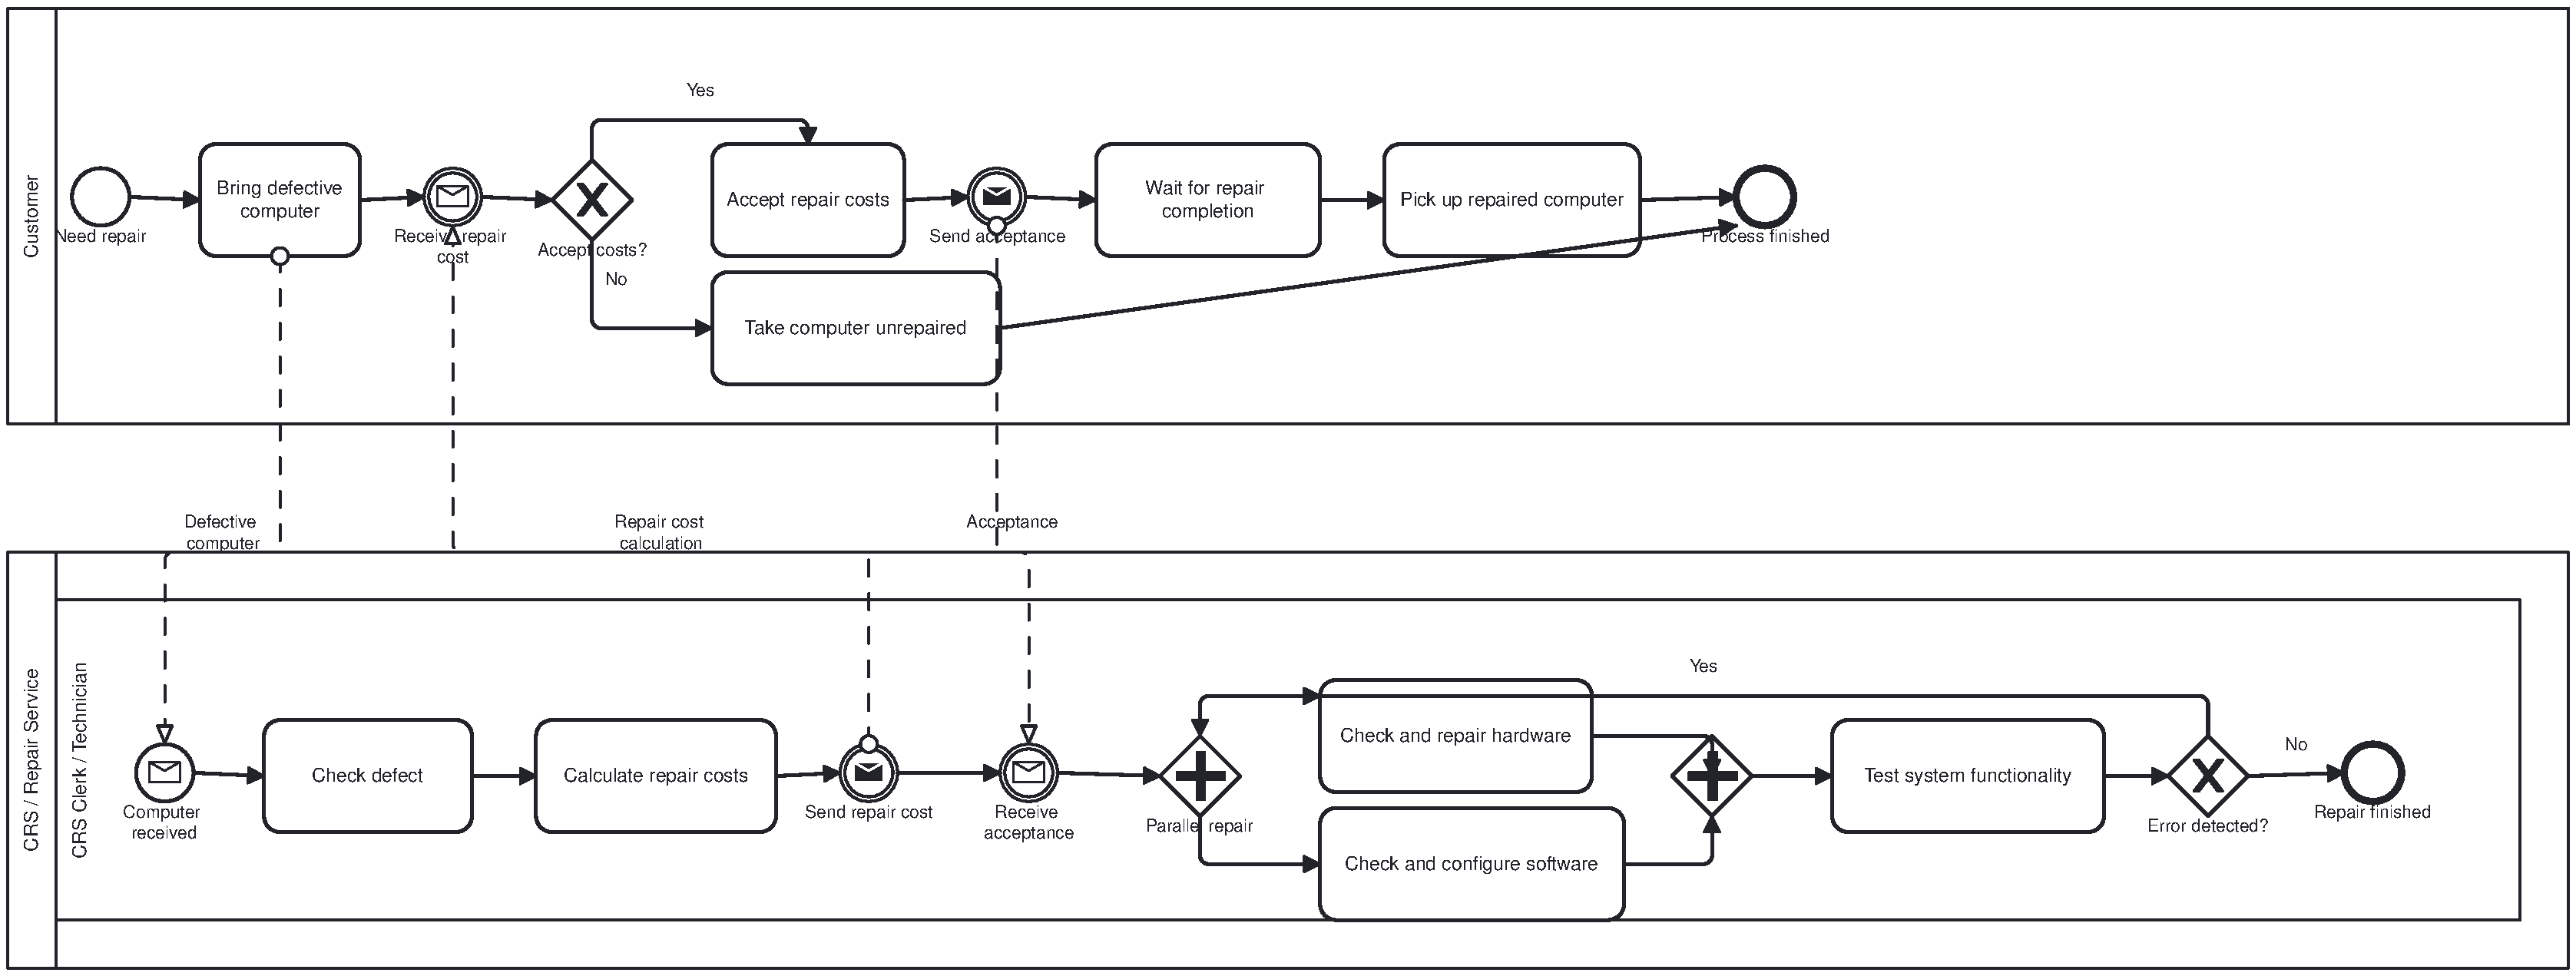
\includegraphics[width=\textwidth]{images/diagrams/gpt-5.1-(xml)-d6bbj9uj}
  \caption{Diagramm von ChatGPT 5.1 mit XML \\ 6347 TOKEN | 0.080 \$ | 83 s}
  \label{fig:gpt-5-1-xml-2}
\end{figure}

\begin{figure}[!htb]
  \centering
  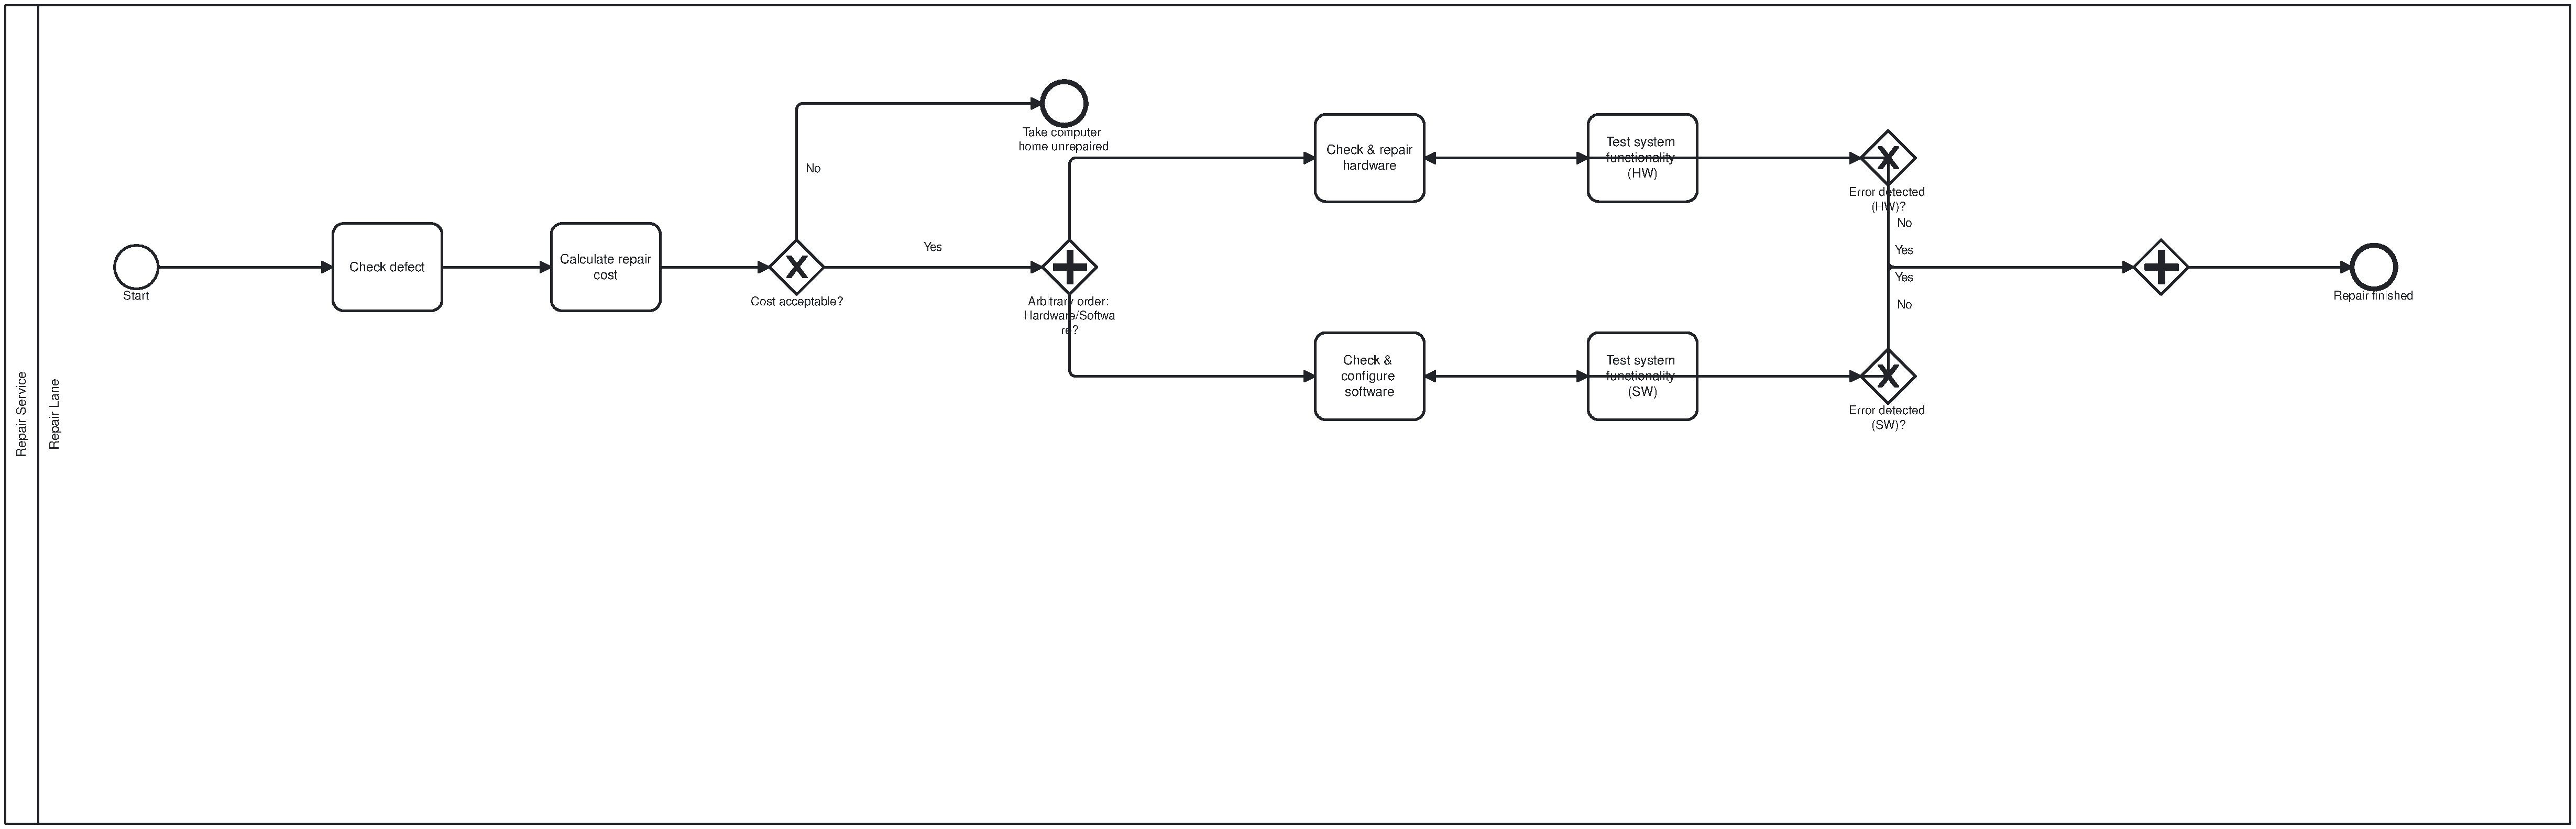
\includegraphics[width=\textwidth]{images/diagrams/gpt-4.1-(json)-ptei22kv}
  \caption{Diagramm von ChatGPT 4.1 mit JSON \\ 2021 TOKEN | 0.040 \$ | 18 s}
  \label{fig:gpt-4-1-json-2}
\end{figure}

\begin{figure}[!htb]
  \centering
  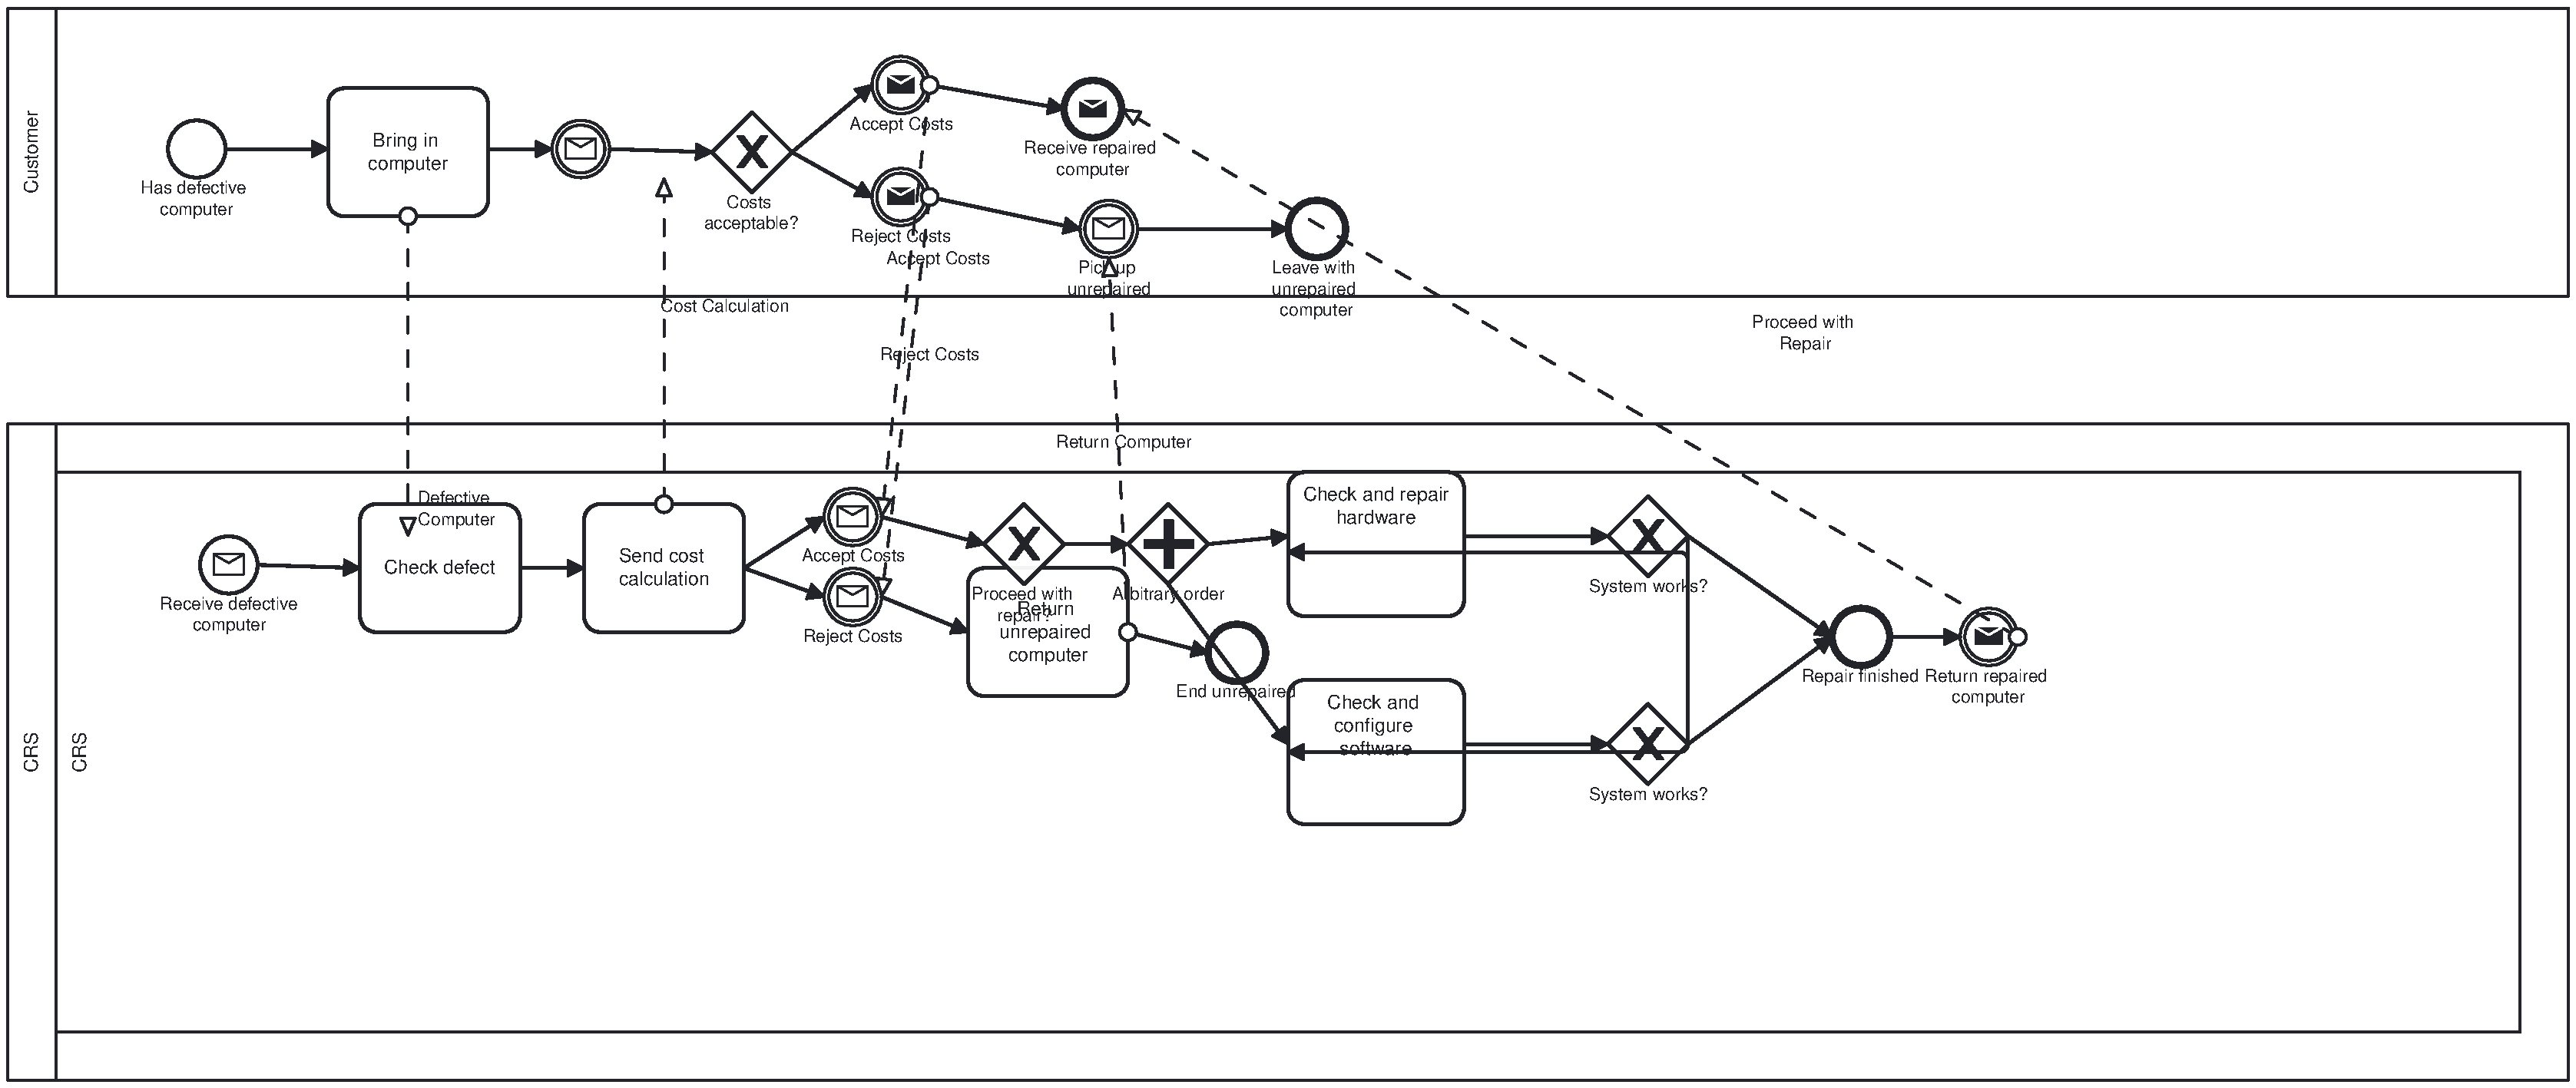
\includegraphics[width=\textwidth]{images/diagrams/gpt-4.1-(xml)-w5mzr01v}
  \caption{Diagramm von ChatGPT 4.1 mit XML \\ 7379 TOKEN | 0.085 \$ | 70 s}
  \label{fig:gpt-4-1-xml-2}
\end{figure}

\begin{figure}[!htb]
  \centering
  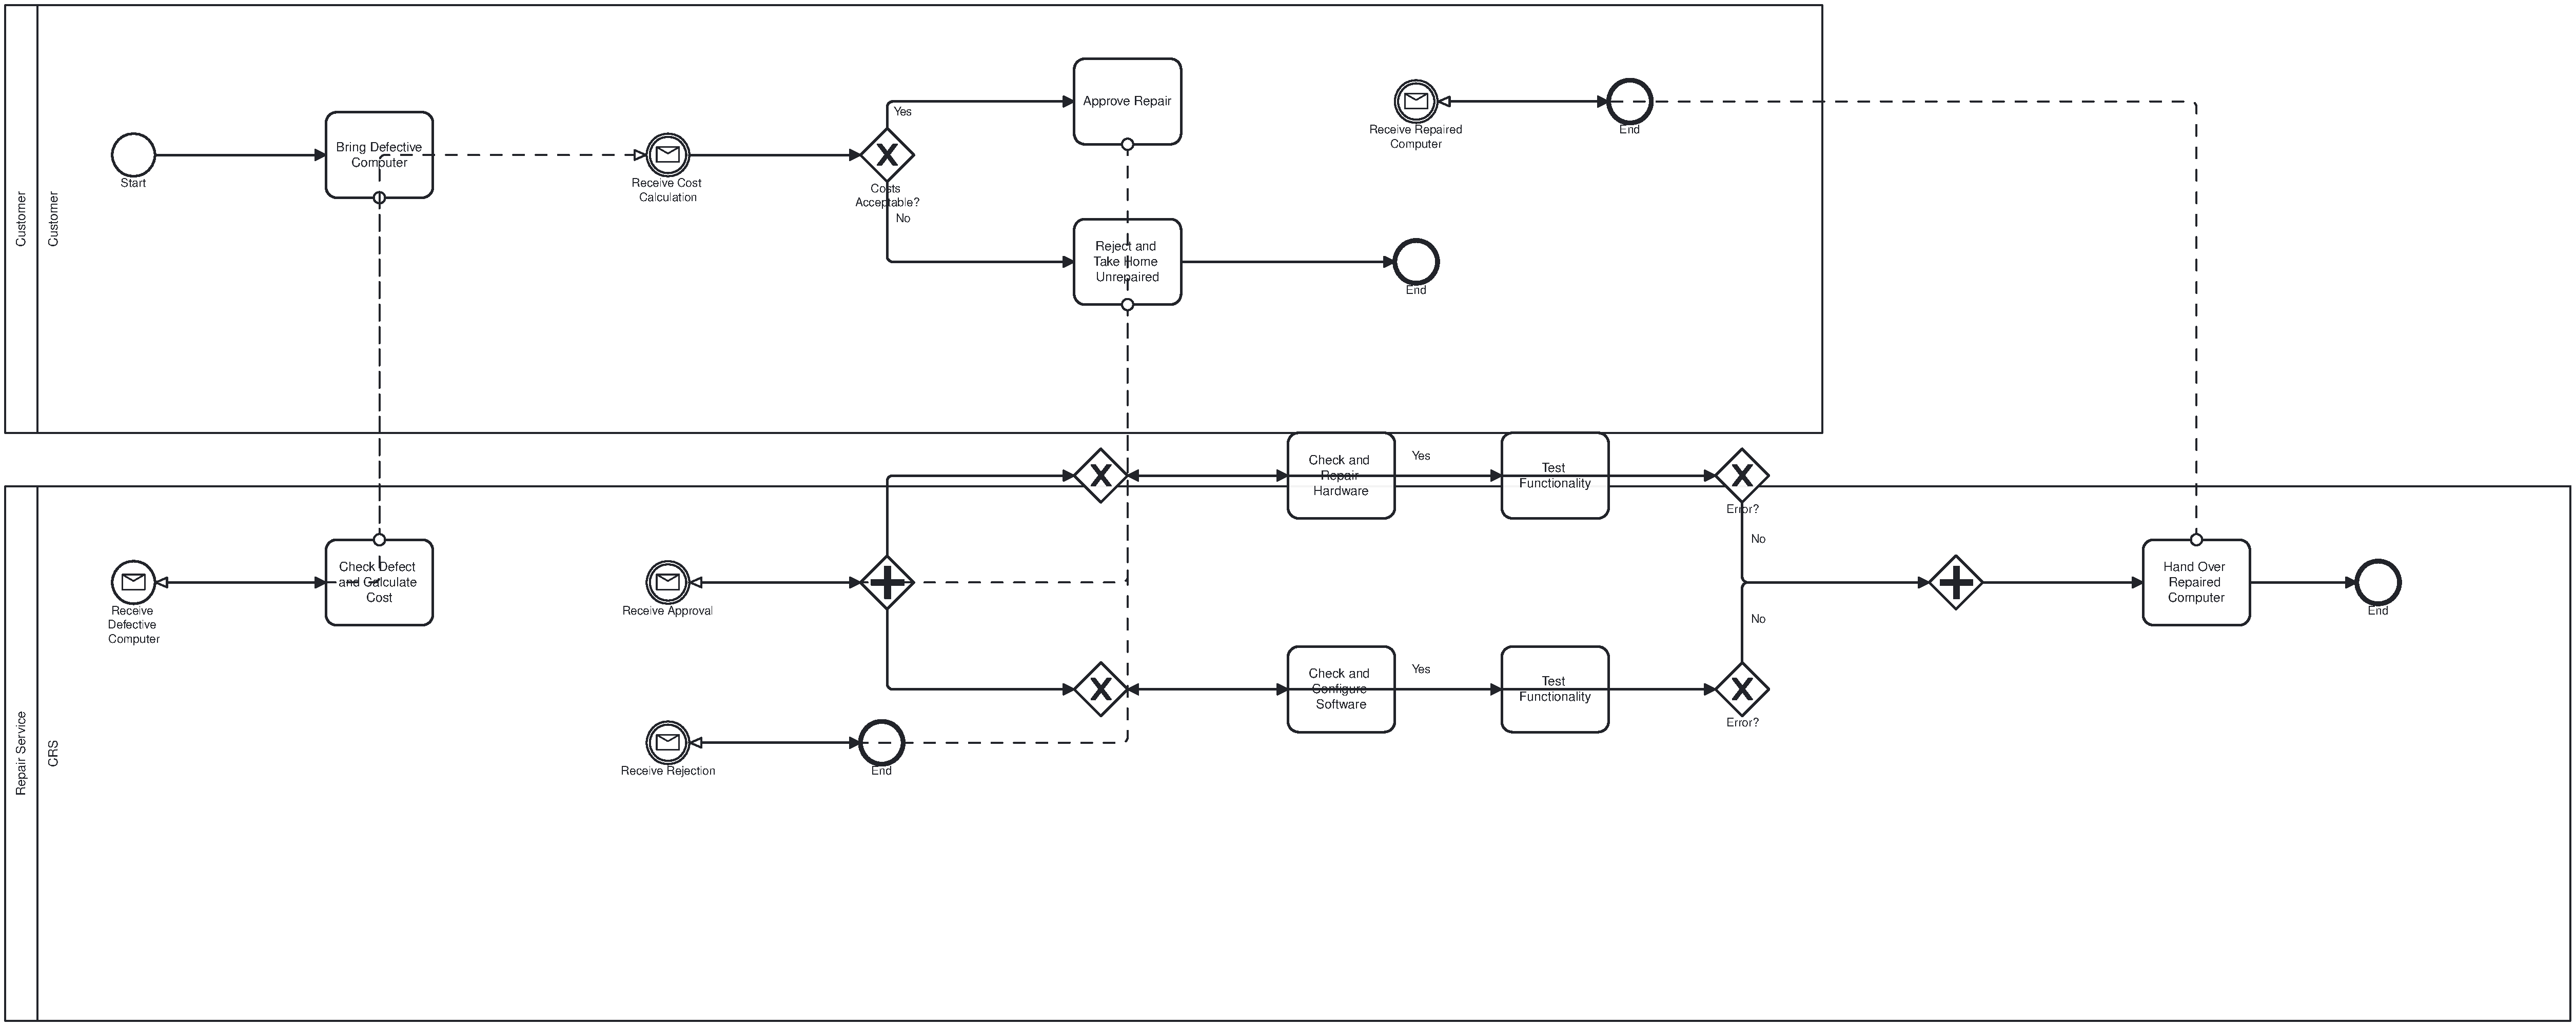
\includegraphics[width=\textwidth]{images/diagrams/grok-4-(json)-q6b4ld1k}
  \caption{Diagramm von Grok 4 mit JSON \\ 3578+3432 TOKEN | 0.143 \$ | 159 s}
  \label{fig:grok-4-json-2}
\end{figure}

\begin{figure}[!htb]
  \centering
  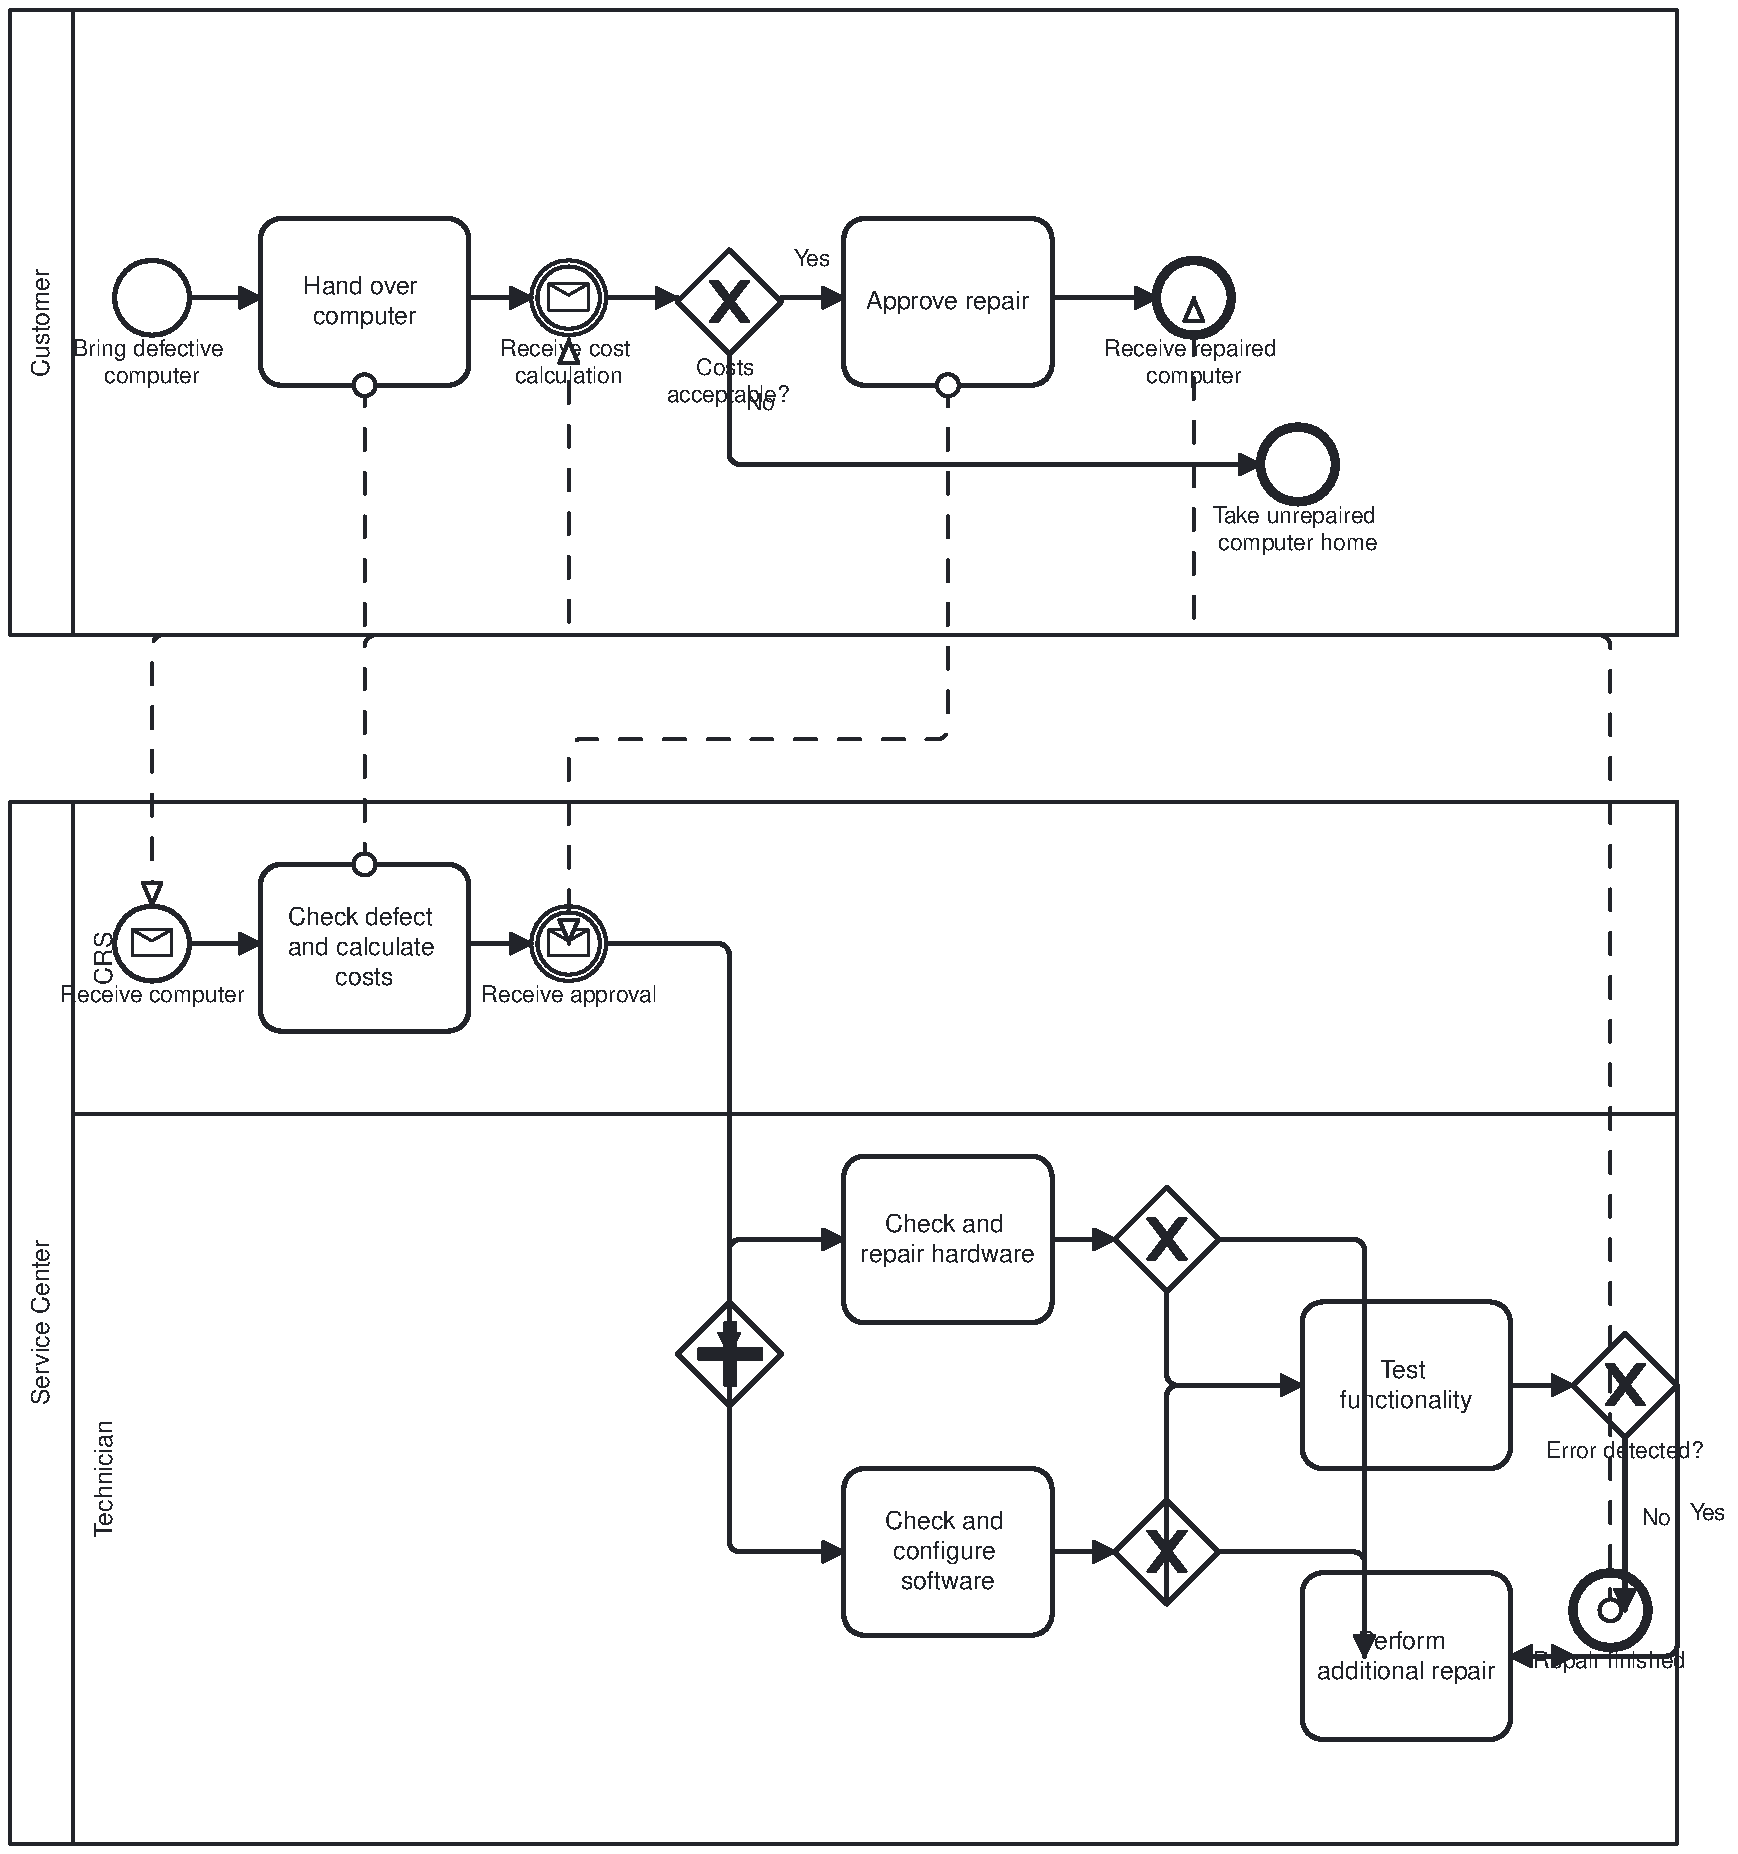
\includegraphics[width=\textwidth]{images/diagrams/grok-4-(xml)-0r9ba3rm}
  \caption{Diagramm von Grok 4 mit XML \\ 5885+780 TOKEN | 0.140 \$ | 162 s}
  \label{fig:grok-4-xml-2}
\end{figure}

\begin{figure}[!htb]
  \centering
  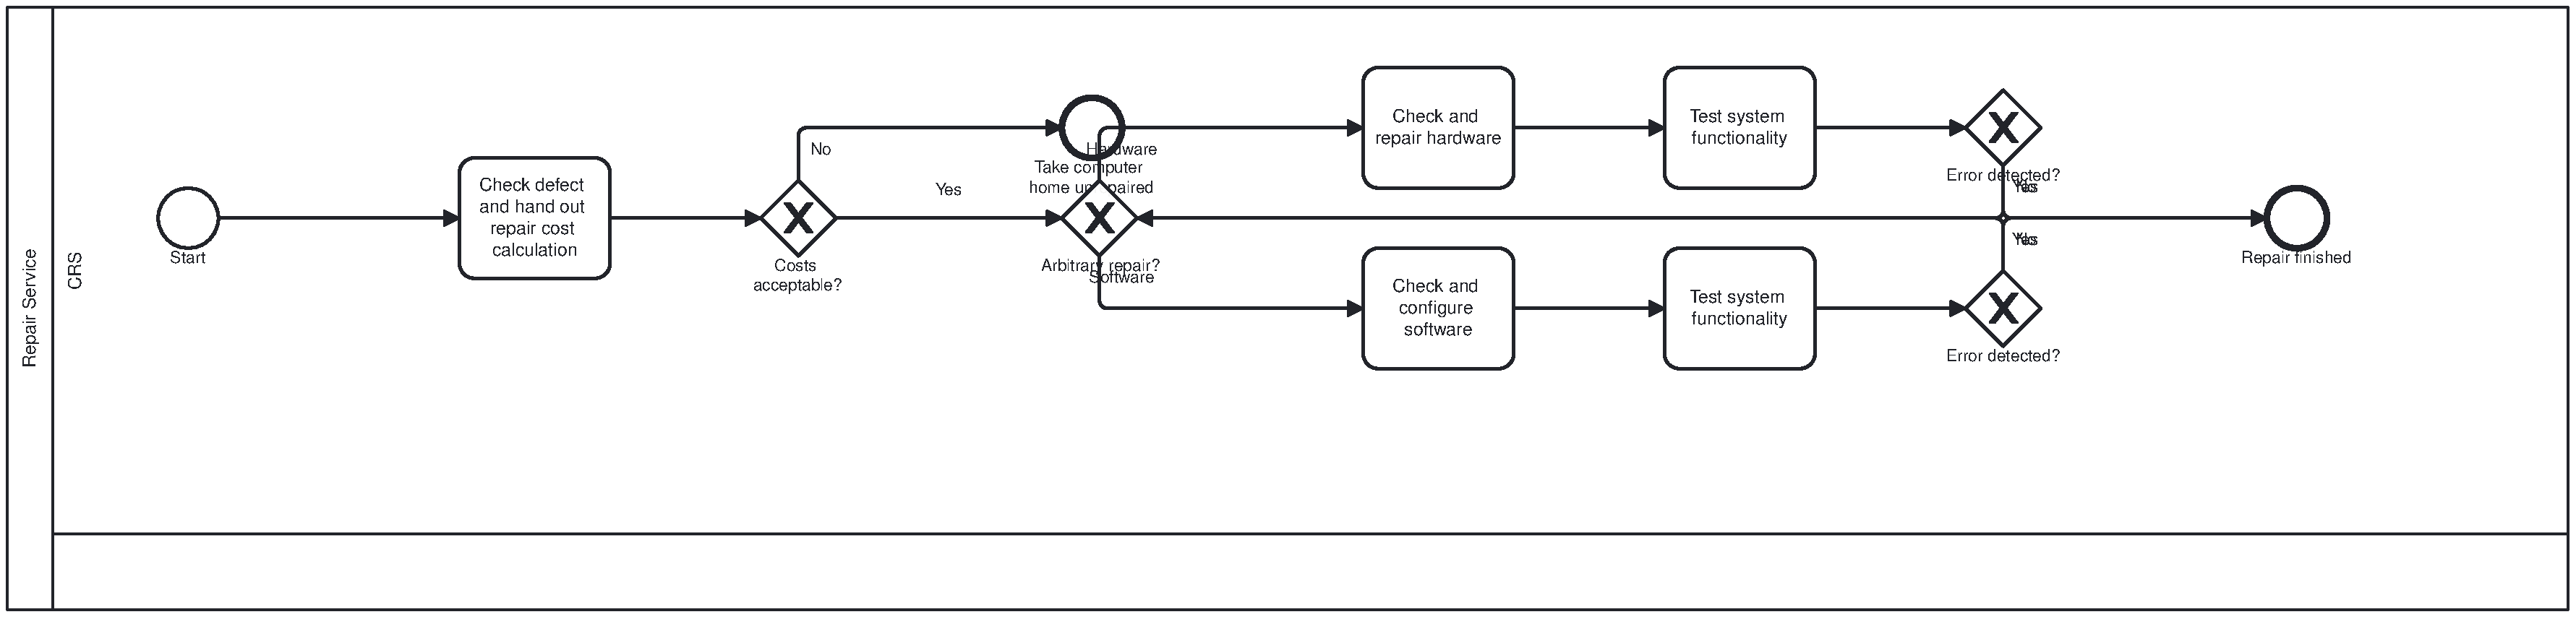
\includegraphics[width=\textwidth]{images/diagrams/grok-4-1-fast-reasoning-(json)-193n5f2e}
  \caption{Diagramm von Grok 4.1 Fast mit JSON \\ 1760+8033 TOKEN | 0.007 \$ | 115 s}
  \label{fig:grok-4-1-json-2}
\end{figure}

\begin{figure}[!htb]
  \centering
  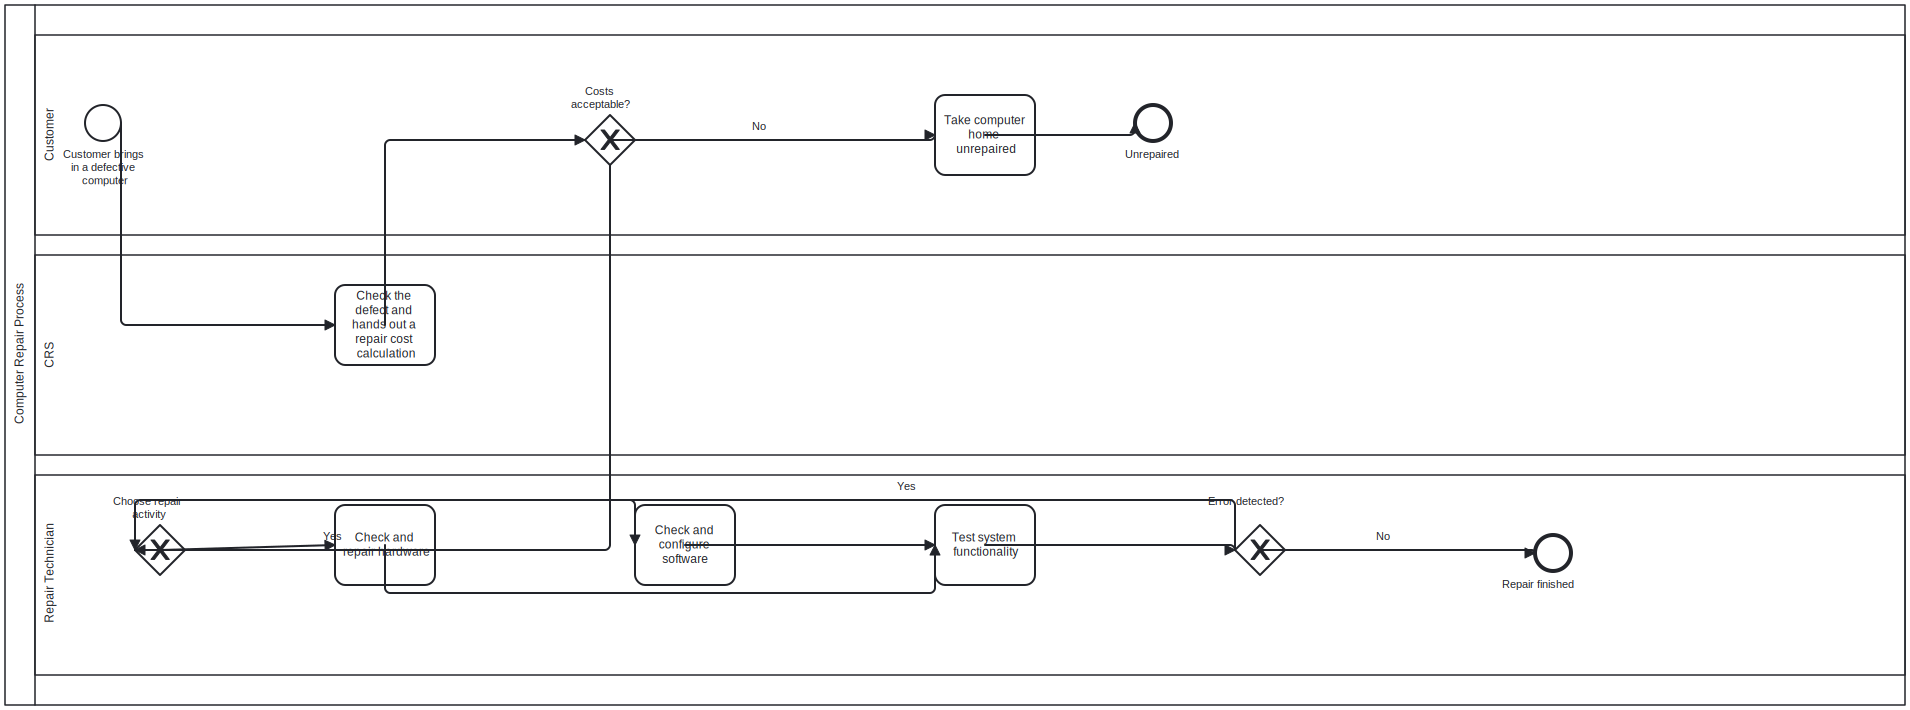
\includegraphics[width=\textwidth]{images/diagrams/grok-4-1-fast-reasoning-(xml)-4wyh07d1}
  \caption{Diagramm von Grok 4.1 Fast mit XML \\ 4254+10244 TOKEN | 0.010 \$ | 126 s}
  \label{fig:grok-4-1-xml-2}
\end{figure}

\begin{figure}[!htb]
  \centering
  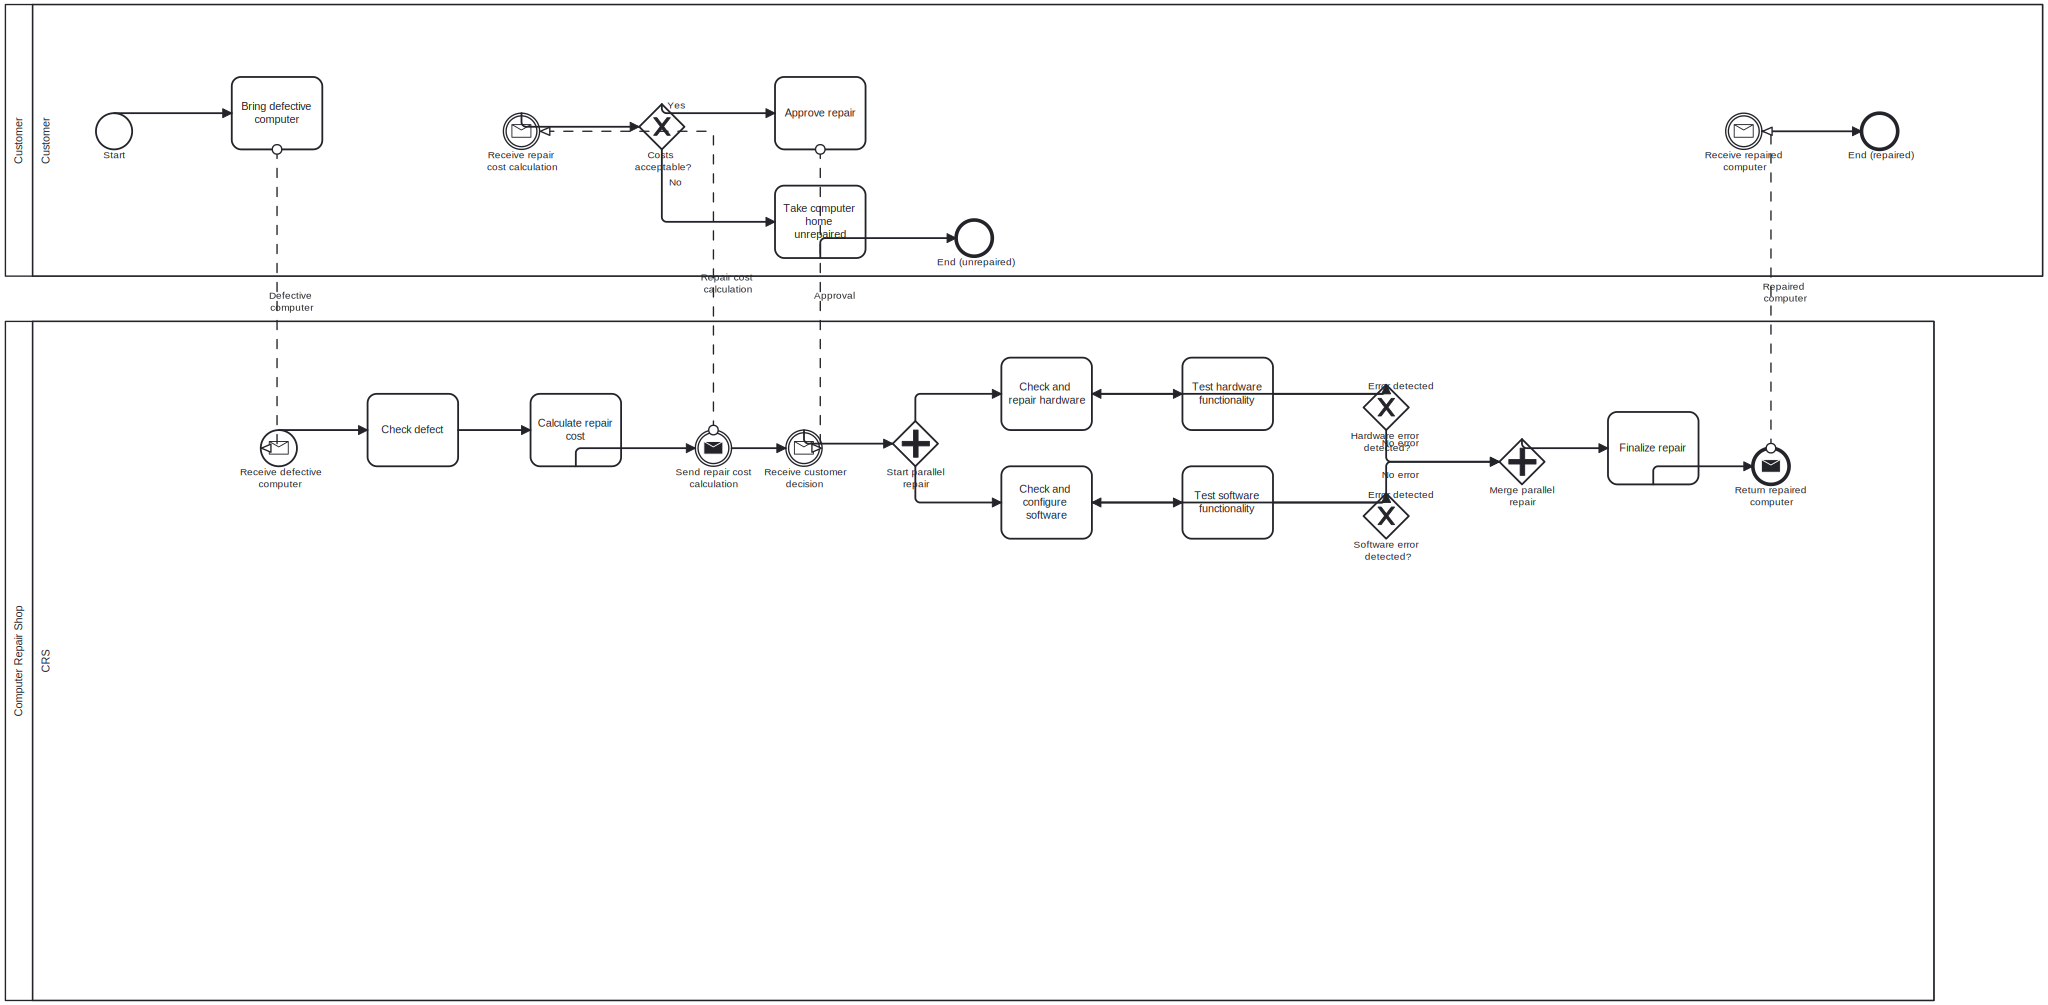
\includegraphics[width=\textwidth]{images/diagrams/claude-opus-4-5-(json)-bmhunnf9}
  \caption{Diagramm von Claude Opus 4.5 mit JSON \\ 4657 TOKEN | 0.190 \$ | 42 s}
  \label{fig:claude-opus-4-5-json-2}
\end{figure}

\begin{figure}[!htb]
  \centering
  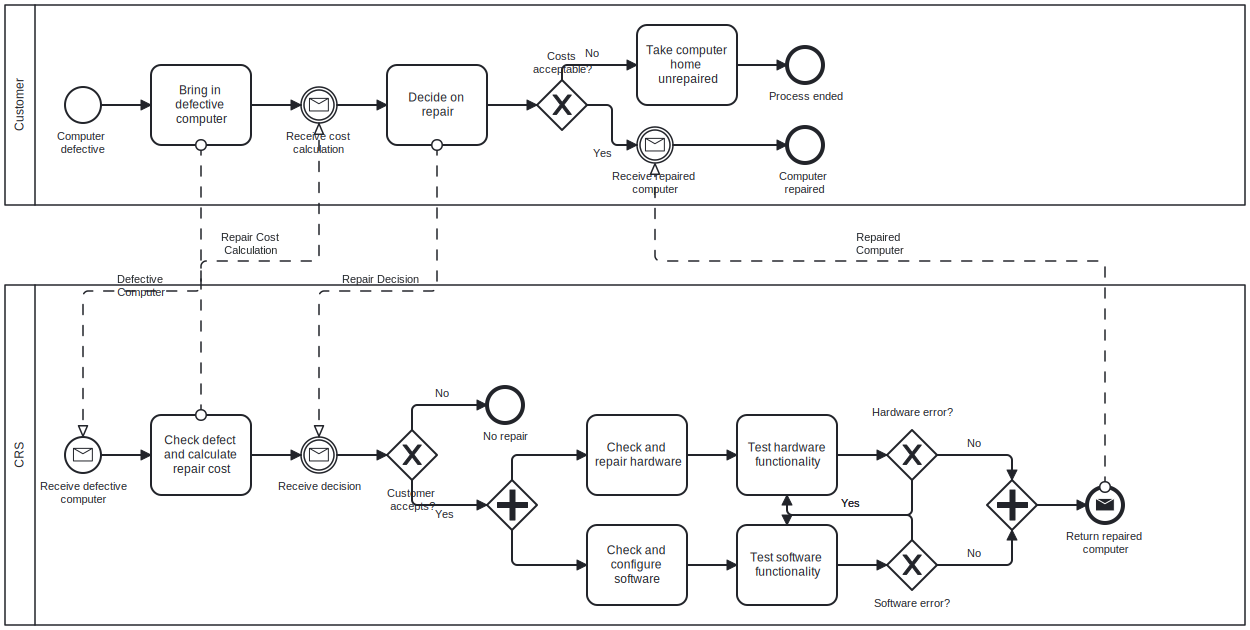
\includegraphics[width=\textwidth]{images/diagrams/claude-opus-4-5-(xml)-gfpum04k}
  \caption{Diagramm von Claude Opus 4.5 mit XML \\ 9531 TOKEN | 0.318 \$ | 74 s}
  \label{fig:claude-opus-4-5-xml-2}
\end{figure}

\begin{figure}[!htb]
  \centering
  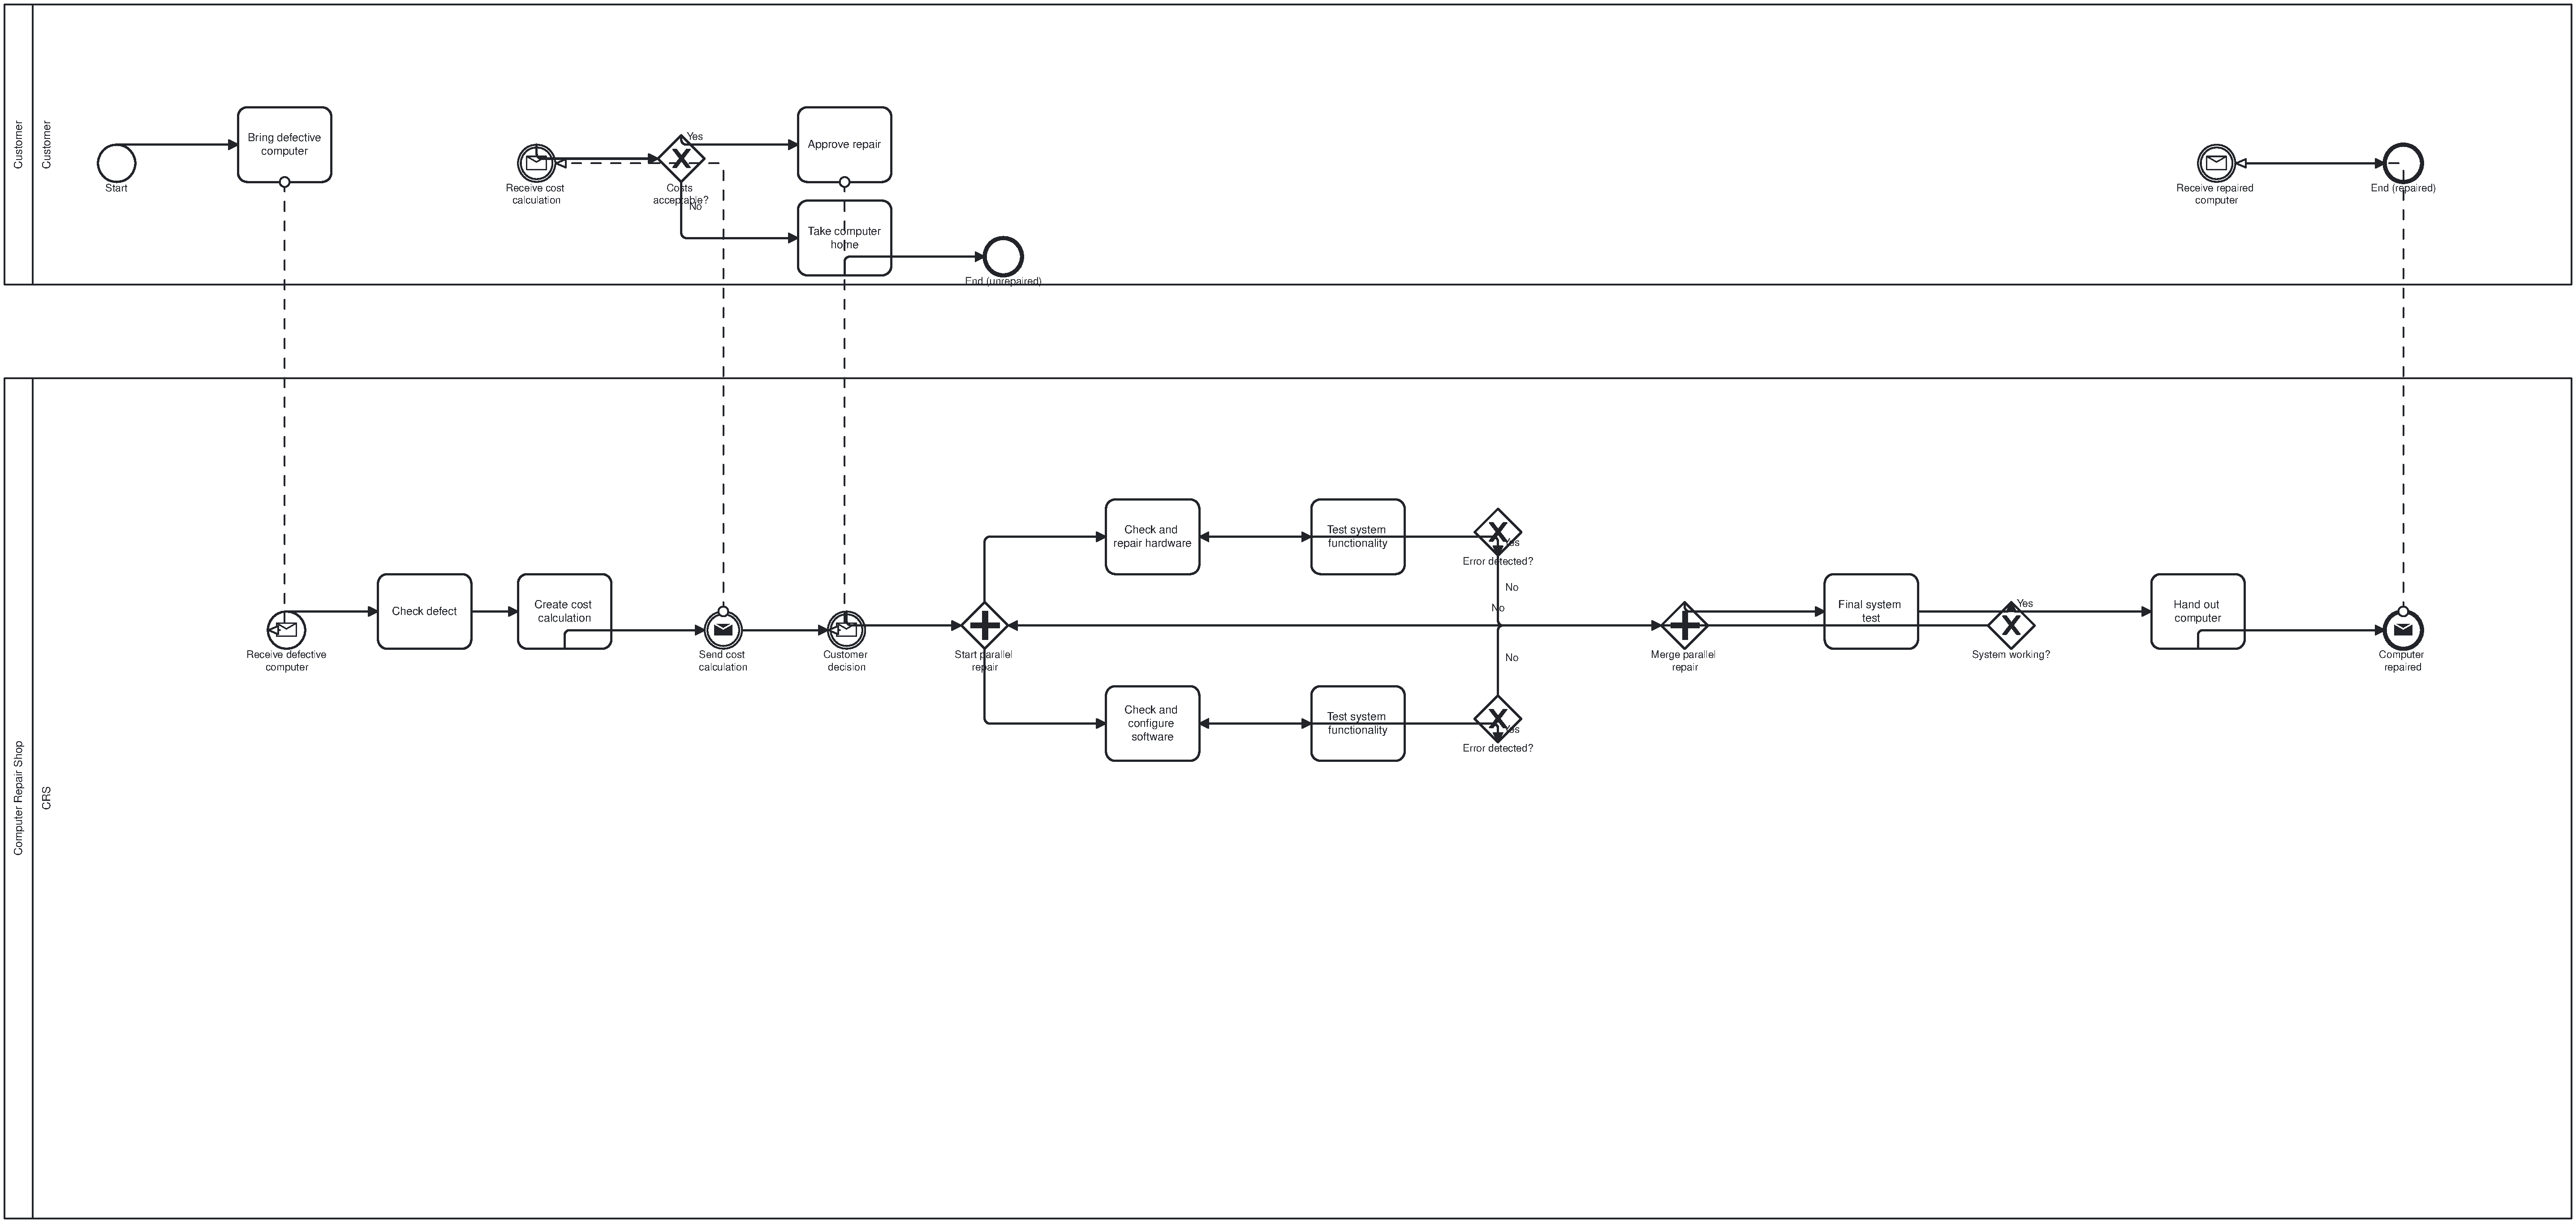
\includegraphics[width=\textwidth]{images/diagrams/claude-sonnet-4-5-(json)-jj1dkubl}
  \caption{Diagramm von Claude Sonnet 4.5 mit JSON \\ 4623 TOKEN | 0.114 \$ | 45 s}
  \label{fig:claude-sonnet-4-5-json-2}
\end{figure}

\begin{figure}[!htb]
  \centering
  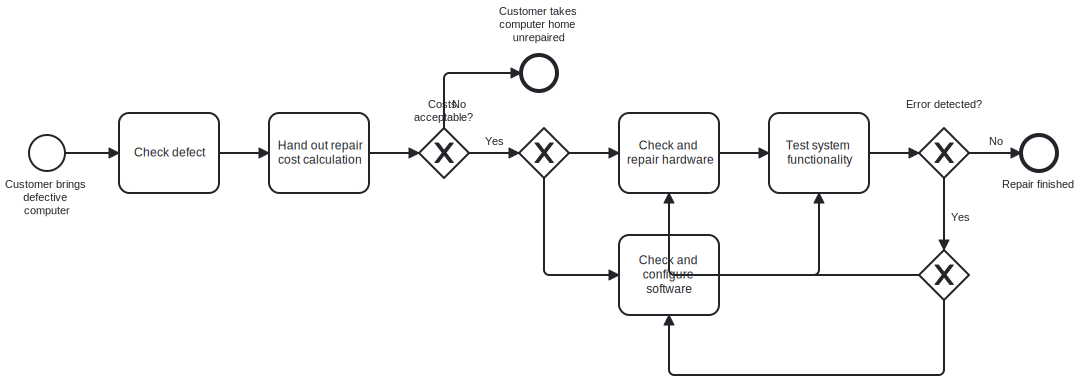
\includegraphics[width=\textwidth]{images/diagrams/claude-sonnet-4-5-(xml)-g4bkm43a}
  \caption{Diagramm von Claude Sonnet 4.5 mit XML \\ 4341 TOKEN | 0.113 \$ | 39 s}
  \label{fig:claude-sonnet-4-5-xml-2}
\end{figure}

% \begin{figure}[!htb]
%   \centering
%   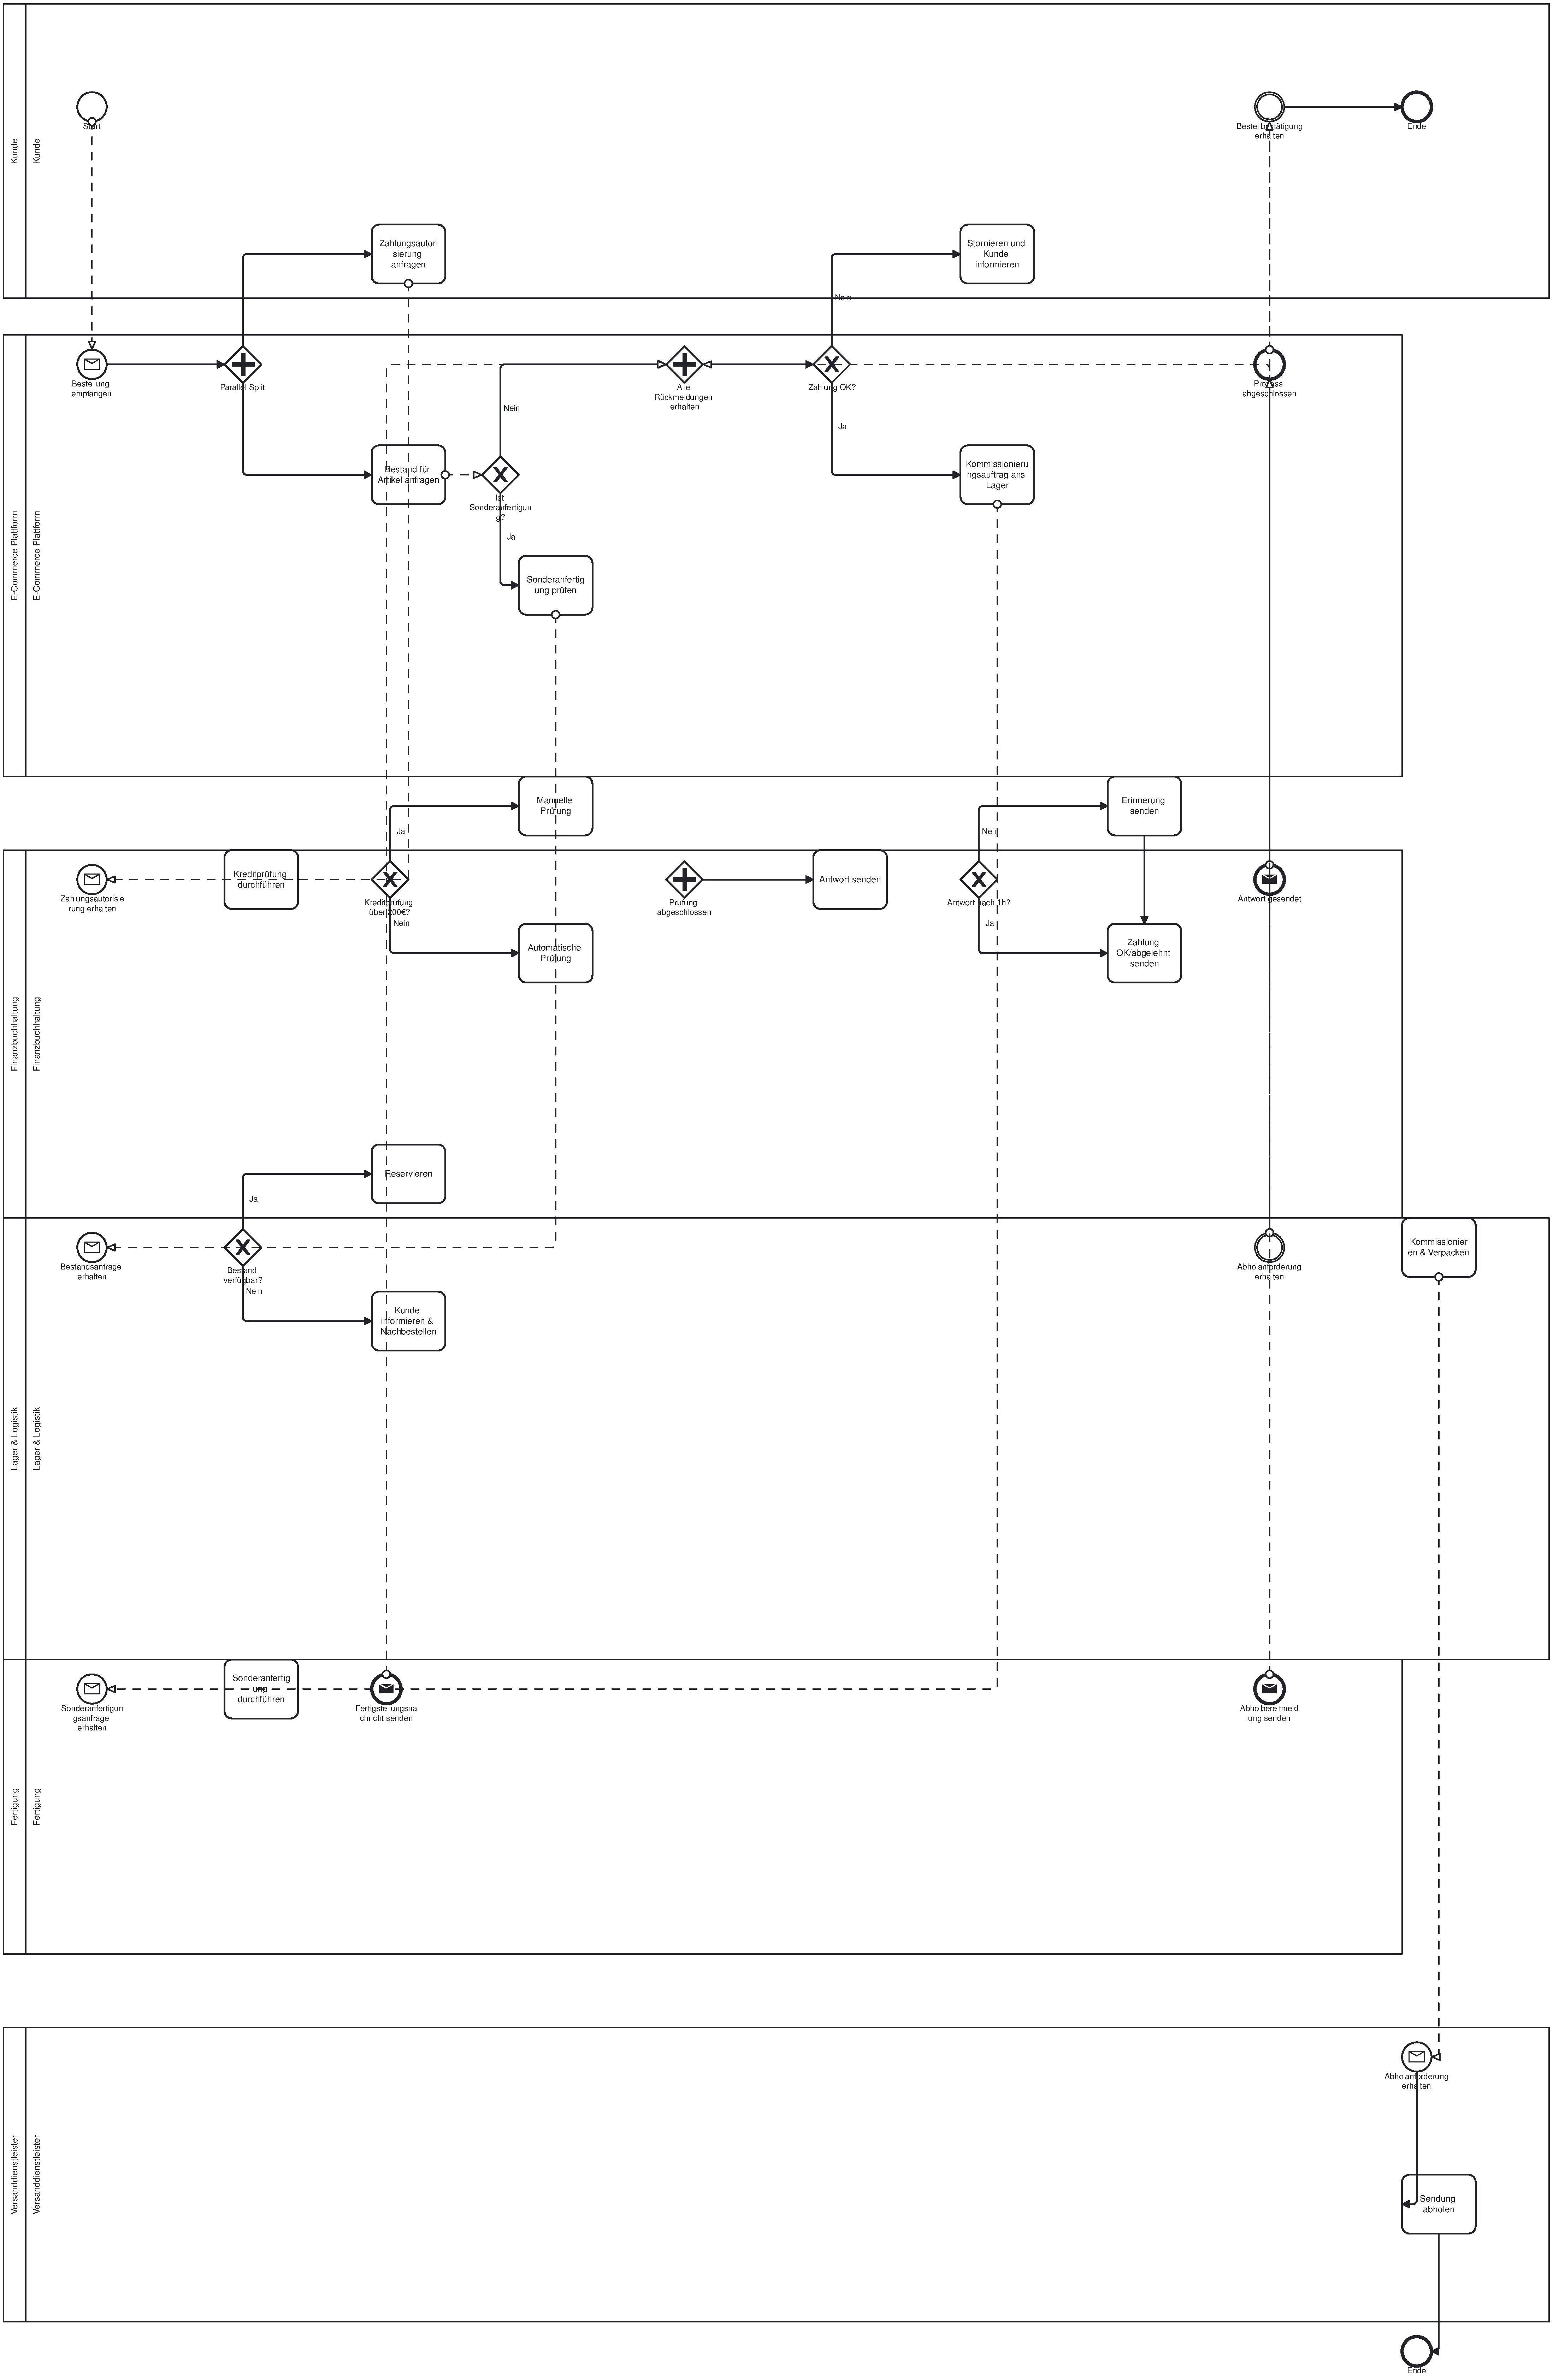
\includegraphics[width=\textwidth]{images/diagrams/assistant-9dkzbc40}
%   \caption{Diagramm vom Assistant mit GPT 4.1 \\ 4230 TOKEN | 6308 \$ | 86 s}
%   \label{fig:assistant-gpt-4-1}
% \end{figure}

% \begin{figure}[!htb]
%   \centering
%   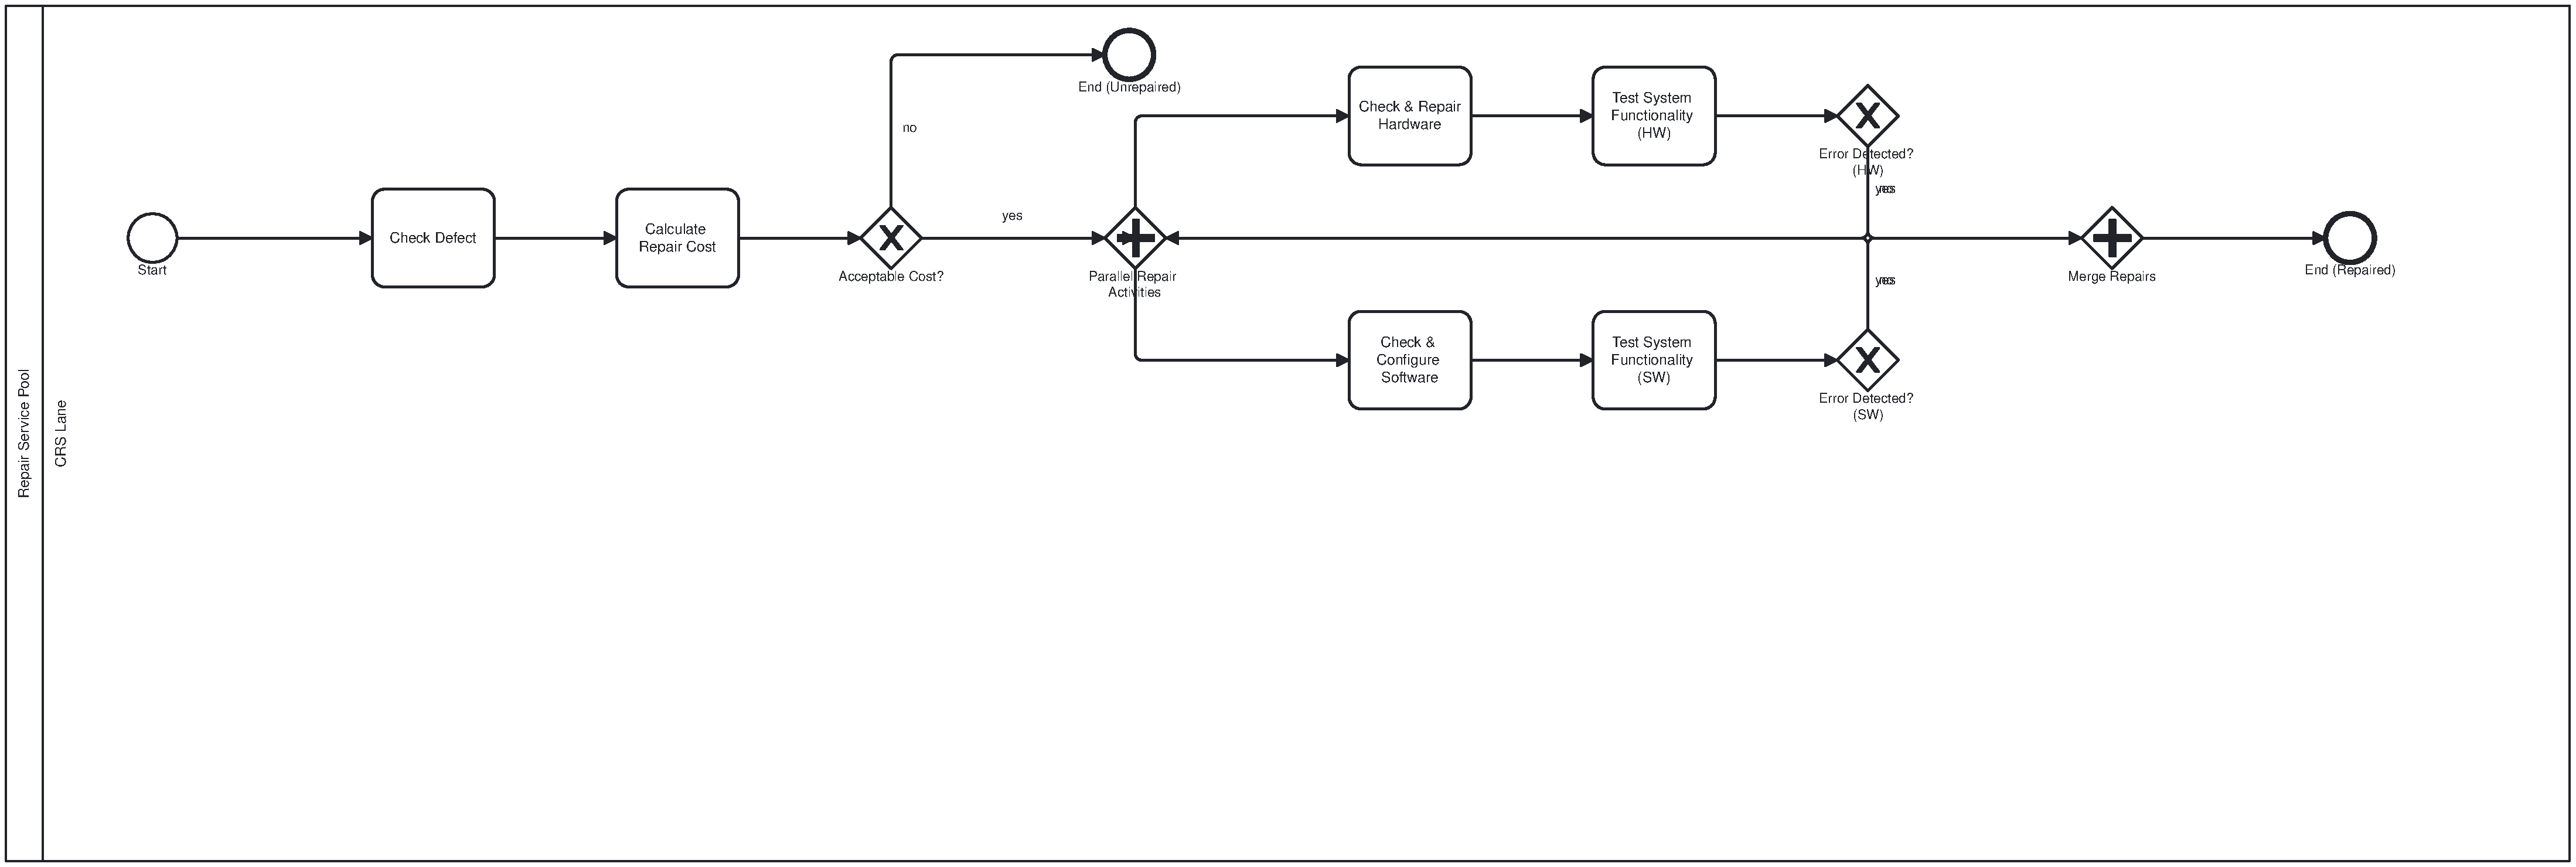
\includegraphics[width=\textwidth]{images/diagrams/assistant-f6g0ajwg}
%   \caption{Diagramm vom Assistant mit GPT 4.1 \\ 2083 TOKEN | 6129 \$ | 33 s}
%   \label{fig:assistant-gpt-4-1-2}
% \end{figure}


